% numbers.tex is generated by paper/scripts/fill_numbers.py from benchmarks/results.json.
\documentclass{aastex631}
\usepackage{amsmath}
\usepackage{booktabs}
\usepackage{array}
\usepackage{graphicx}
\usepackage{placeins}  % \FloatBarrier at the section breaks keeps each figure and table in the section that cites it
% written by scripts/fill_numbers.py from benchmarks/results.json
\expandafter\def\csname t@astropy@20000\endcsname{37.2}
\expandafter\def\csname p@astropy@20000\endcsname{91\,607}
\expandafter\def\csname t@astropy@100000\endcsname{51.3}
\expandafter\def\csname p@astropy@100000\endcsname{91\,607}
\expandafter\def\csname t@astropy@200000\endcsname{69.1}
\expandafter\def\csname p@astropy@200000\endcsname{91\,607}
\expandafter\def\csname t@gpu@20000\endcsname{0.267}
\expandafter\def\csname p@gpu@20000\endcsname{91\,607}
\expandafter\def\csname t@gpu@72000\endcsname{0.951}
\expandafter\def\csname p@gpu@72000\endcsname{191\,837}
\expandafter\def\csname t@gpu@100000\endcsname{0.505}
\expandafter\def\csname p@gpu@100000\endcsname{91\,607}
\expandafter\def\csname t@gpu@144000\endcsname{2.91}
\expandafter\def\csname p@gpu@144000\endcsname{391\,781}
\expandafter\def\csname t@gpu@200000\endcsname{0.579}
\expandafter\def\csname p@gpu@200000\endcsname{91\,607}
\expandafter\def\csname t@gpu-shuffles@20000\endcsname{5.21}
\expandafter\def\csname p@gpu-shuffles@20000\endcsname{4\,397\,136}
\expandafter\def\csname t@gpu-shuffles@100000\endcsname{6.95}
\expandafter\def\csname p@gpu-shuffles@100000\endcsname{4\,397\,136}
\expandafter\def\csname t@gpu-shuffles@200000\endcsname{9.86}
\expandafter\def\csname p@gpu-shuffles@200000\endcsname{4\,397\,136}
\expandafter\def\csname t@hybrid@20000\endcsname{0.443}
\expandafter\def\csname p@hybrid@20000\endcsname{91\,607}
\expandafter\def\csname t@hybrid@100000\endcsname{0.874}
\expandafter\def\csname p@hybrid@100000\endcsname{91\,607}
\expandafter\def\csname t@hybrid@200000\endcsname{1.24}
\expandafter\def\csname p@hybrid@200000\endcsname{91\,607}
\expandafter\def\csname t@many@20000\endcsname{6.90}
\expandafter\def\csname p@many@20000\endcsname{5\,862\,848}
\expandafter\def\csname t@tls-gpu@20000\endcsname{2.48}
\expandafter\def\csname p@tls-gpu@20000\endcsname{91\,607}
\expandafter\def\csname t@tls-gpu@72000\endcsname{18.2}
\expandafter\def\csname p@tls-gpu@72000\endcsname{191\,837}
\expandafter\def\csname t@tls-gpu@100000\endcsname{5.55}
\expandafter\def\csname p@tls-gpu@100000\endcsname{91\,607}
\expandafter\def\csname t@tls-gpu@144000\endcsname{57.0}
\expandafter\def\csname p@tls-gpu@144000\endcsname{391\,781}
\expandafter\def\csname t@tls-gpu@200000\endcsname{10.8}
\expandafter\def\csname p@tls-gpu@200000\endcsname{91\,607}
\expandafter\def\csname t@tls-gpu-binned@20000\endcsname{1.08}
\expandafter\def\csname p@tls-gpu-binned@20000\endcsname{91\,607}
\expandafter\def\csname t@tls-gpu-binned@72000\endcsname{5.98}
\expandafter\def\csname p@tls-gpu-binned@72000\endcsname{191\,837}
\expandafter\def\csname t@tls-gpu-binned@100000\endcsname{1.32}
\expandafter\def\csname p@tls-gpu-binned@100000\endcsname{91\,607}
\expandafter\def\csname t@tls-gpu-binned@144000\endcsname{14.0}
\expandafter\def\csname p@tls-gpu-binned@144000\endcsname{391\,781}
\expandafter\def\csname t@tls-gpu-binned@200000\endcsname{1.42}
\expandafter\def\csname p@tls-gpu-binned@200000\endcsname{91\,607}
\expandafter\def\csname t@tls-gpu-margin@72000\endcsname{7.54}
\expandafter\def\csname p@tls-gpu-margin@72000\endcsname{191\,837}
\expandafter\def\csname t@tls-gpu-margin@144000\endcsname{25.4}
\expandafter\def\csname p@tls-gpu-margin@144000\endcsname{391\,781}
\expandafter\def\csname t@tls-gpu-pl@20000\endcsname{1.17}
\expandafter\def\csname p@tls-gpu-pl@20000\endcsname{91\,607}
\expandafter\def\csname t@tls-gpu-pl@100000\endcsname{3.84}
\expandafter\def\csname p@tls-gpu-pl@100000\endcsname{91\,607}
\expandafter\def\csname t@tls-gpu-pl@200000\endcsname{6.45}
\expandafter\def\csname p@tls-gpu-pl@200000\endcsname{91\,607}
\expandafter\def\csname t@tls1@20000\endcsname{20.2}
\expandafter\def\csname p@tls1@20000\endcsname{91\,607}
\expandafter\def\csname t@tls1@100000\endcsname{49.1}
\expandafter\def\csname p@tls1@100000\endcsname{91\,607}
\expandafter\def\csname t@tls1@200000\endcsname{85.6}
\expandafter\def\csname p@tls1@200000\endcsname{91\,607}
\expandafter\def\csname t@tls1-exact@20000\endcsname{91.0}
\expandafter\def\csname p@tls1-exact@20000\endcsname{91\,607}
\expandafter\def\csname t@tls1-exact@100000\endcsname{166}
\expandafter\def\csname p@tls1-exact@100000\endcsname{91\,607}
\expandafter\def\csname t@tls1-exact@200000\endcsname{277}
\expandafter\def\csname p@tls1-exact@200000\endcsname{91\,607}
\expandafter\def\csname t@tls16@20000\endcsname{1.45}
\expandafter\def\csname p@tls16@20000\endcsname{91\,607}
\expandafter\def\csname t@tls16@100000\endcsname{4.06}
\expandafter\def\csname p@tls16@100000\endcsname{91\,607}
\expandafter\def\csname t@tls16@200000\endcsname{10.8}
\expandafter\def\csname p@tls16@200000\endcsname{91\,607}
\expandafter\def\csname t@tls16-exact@20000\endcsname{6.43}
\expandafter\def\csname p@tls16-exact@20000\endcsname{91\,607}
\expandafter\def\csname t@tls16-exact@72000\endcsname{37.2}
\expandafter\def\csname p@tls16-exact@72000\endcsname{191\,837}
\expandafter\def\csname t@tls16-exact@100000\endcsname{12.4}
\expandafter\def\csname p@tls16-exact@100000\endcsname{91\,607}
\expandafter\def\csname t@tls16-exact@144000\endcsname{128}
\expandafter\def\csname p@tls16-exact@144000\endcsname{391\,781}
\expandafter\def\csname t@tls16-exact@200000\endcsname{26.6}
\expandafter\def\csname p@tls16-exact@200000\endcsname{91\,607}
\expandafter\def\csname t@tls16-exact-margin@72000\endcsname{9.11}
\expandafter\def\csname p@tls16-exact-margin@72000\endcsname{191\,837}
\expandafter\def\csname t@tls16-exact-margin@144000\endcsname{44.2}
\expandafter\def\csname p@tls16-exact-margin@144000\endcsname{391\,781}
\expandafter\def\csname t@tls16-many@20000\endcsname{92.4}
\expandafter\def\csname p@tls16-many@20000\endcsname{5\,862\,848}
\expandafter\def\csname r@tls16@gpu@20000\endcsname{5.4}
\expandafter\def\csname r@tls16@gpu@100000\endcsname{8}
\expandafter\def\csname r@tls16@gpu@200000\endcsname{19}
\expandafter\def\csname r@tls16-exact@tls-gpu@20000\endcsname{2.6}
\expandafter\def\csname r@tls16-exact@tls-gpu@72000\endcsname{2}
\expandafter\def\csname r@tls16-exact@tls-gpu@100000\endcsname{2.2}
\expandafter\def\csname r@tls16-exact@tls-gpu@144000\endcsname{2.2}
\expandafter\def\csname r@tls16-exact@tls-gpu@200000\endcsname{2.5}
\expandafter\def\csname r@tls16@tls-gpu-binned@20000\endcsname{1.4}
\expandafter\def\csname r@tls16@tls-gpu-binned@100000\endcsname{3.1}
\expandafter\def\csname r@tls16@tls-gpu-binned@200000\endcsname{7.6}
\expandafter\def\csname r@tls1@gpu@20000\endcsname{76}
\expandafter\def\csname r@tls1@gpu@100000\endcsname{97}
\expandafter\def\csname r@tls1@gpu@200000\endcsname{148}
\expandafter\def\csname r@tls1-exact@tls-gpu@20000\endcsname{37}
\expandafter\def\csname r@tls1-exact@tls-gpu@100000\endcsname{30}
\expandafter\def\csname r@tls1-exact@tls-gpu@200000\endcsname{26}
\expandafter\def\csname r@astropy@gpu@20000\endcsname{139}
\expandafter\def\csname r@astropy@gpu@100000\endcsname{102}
\expandafter\def\csname r@astropy@gpu@200000\endcsname{119}
\expandafter\def\csname r@tls-gpu@gpu@20000\endcsname{9.3}
\expandafter\def\csname r@tls-gpu@gpu@72000\endcsname{19}
\expandafter\def\csname r@tls-gpu@gpu@100000\endcsname{11}
\expandafter\def\csname r@tls-gpu@gpu@144000\endcsname{20}
\expandafter\def\csname r@tls-gpu@gpu@200000\endcsname{19}
\expandafter\def\csname r@tls-gpu@tls-gpu-binned@20000\endcsname{2.3}
\expandafter\def\csname r@tls-gpu@tls-gpu-binned@72000\endcsname{3}
\expandafter\def\csname r@tls-gpu@tls-gpu-binned@100000\endcsname{4.2}
\expandafter\def\csname r@tls-gpu@tls-gpu-binned@144000\endcsname{4.1}
\expandafter\def\csname r@tls-gpu@tls-gpu-binned@200000\endcsname{7.6}
\expandafter\def\csname r@tls16@hybrid@20000\endcsname{3.3}
\expandafter\def\csname r@tls16@hybrid@100000\endcsname{4.6}
\expandafter\def\csname r@tls16@hybrid@200000\endcsname{8.7}
\expandafter\def\csname r@tls16-many@many@20000\endcsname{13}
\expandafter\def\csname r@tls16-exact-margin@tls-gpu-margin@72000\endcsname{1.2}
\expandafter\def\csname r@tls16-exact-margin@tls-gpu-margin@144000\endcsname{1.7}
\expandafter\def\csname r@tls16-exact@tls-gpu-binned@20000\endcsname{6}
\expandafter\def\csname r@tls16-exact@tls-gpu-binned@72000\endcsname{6.2}
\expandafter\def\csname r@tls16-exact@tls-gpu-binned@100000\endcsname{9.4}
\expandafter\def\csname r@tls16-exact@tls-gpu-binned@144000\endcsname{9.1}
\expandafter\def\csname r@tls16-exact@tls-gpu-binned@200000\endcsname{19}
\expandafter\def\csname h@cpu\endcsname{AMD Ryzen 9 9950X3D 16-Core Processor}
\expandafter\def\csname h@logical_cpus\endcsname{32}
\expandafter\def\csname h@gpu\endcsname{AMD Radeon RX 7900 XTX}
\expandafter\def\csname h@gpu_runtime\endcsname{ROCm 7.2.53211}
\expandafter\def\csname v@python\endcsname{3.12.13}
\expandafter\def\csname v@numpy\endcsname{2.5.4}
\expandafter\def\csname v@torch\endcsname{2.12.0+rocm7.2}
\expandafter\def\csname v@astropy\endcsname{8.0.1}
\expandafter\def\csname v@transitleastsquares\endcsname{2.0.1}
\expandafter\def\csname v@numba\endcsname{0.68.0}
\expandafter\def\csname v@triton\endcsname{3.7.0}
\expandafter\def\csname v@batman\endcsname{2.5.3}
\expandafter\def\csname v@wotan\endcsname{1.10}
\providecommand{\Gt}[2]{\ifcsname gt@#1@#2\endcsname\csname gt@#1@#2\endcsname\else[\texttt{#1,#2}]\fi}
\expandafter\def\csname gt@time@72000\endcsname{33.3}
\expandafter\def\csname gt@tls@72000\endcsname{522}
\expandafter\def\csname gt@ratio@72000\endcsname{4.4}
\expandafter\def\csname gt@tlsratio@72000\endcsname{57}
\expandafter\def\csname gt@time@144000\endcsname{138}
\expandafter\def\csname gt@tls@144000\endcsname{3\,289}
\expandafter\def\csname gt@ratio@144000\endcsname{5.4}
\expandafter\def\csname gt@tlsratio@144000\endcsname{74}
\providecommand{\Cold}[2]{\ifcsname cold@#1@#2\endcsname\csname cold@#1@#2\endcsname\else[\texttt{#1,#2}]\fi}
\expandafter\def\csname cold@gpu@kept\endcsname{2.71}
\expandafter\def\csname cold@hybrid@kept\endcsname{2.62}
\expandafter\def\csname cold@many@kept\endcsname{2.18}
\expandafter\def\csname cold@tls-gpu-binned@kept\endcsname{1.18}
\expandafter\def\csname cold@tls-gpu-pl@kept\endcsname{0.844}
\expandafter\def\csname cold@tls-gpu@kept\endcsname{1.42}
\expandafter\def\csname cold@gpu@cleared\endcsname{2.87}
\expandafter\def\csname cold@many@cleared\endcsname{18.1}
\expandafter\def\csname cold@tls-gpu@cleared\endcsname{2.26}

\IfFileExists{threshold_numbers.tex}{% written by scripts/fill_numbers.py from threshold.json
\expandafter\def\csname th@red@above\endcsname{16}
\expandafter\def\csname th@red@of\endcsname{2000}
\expandafter\def\csname th@red@share\endcsname{0.8}
\expandafter\def\csname th@red@low\endcsname{0.5}
\expandafter\def\csname th@red@high\endcsname{1.3}
\expandafter\def\csname th@variable@above\endcsname{1325}
\expandafter\def\csname th@variable@of\endcsname{2000}
\expandafter\def\csname th@variable@share\endcsname{66.2}
\expandafter\def\csname th@variable@low\endcsname{64.1}
\expandafter\def\csname th@variable@high\endcsname{68.3}
\expandafter\def\csname th@white@above\endcsname{50}
\expandafter\def\csname th@white@of\endcsname{2000}
\expandafter\def\csname th@white@share\endcsname{2.5}
\expandafter\def\csname th@white@low\endcsname{1.9}
\expandafter\def\csname th@white@high\endcsname{3.3}
\expandafter\def\csname thi@red@above\endcsname{29}
\expandafter\def\csname thi@red@of\endcsname{2000}
\expandafter\def\csname thi@red@share\endcsname{1.5}
\expandafter\def\csname thi@red@low\endcsname{1.0}
\expandafter\def\csname thi@red@high\endcsname{2.1}
\expandafter\def\csname thi@variable@above\endcsname{1255}
\expandafter\def\csname thi@variable@of\endcsname{2000}
\expandafter\def\csname thi@variable@share\endcsname{62.7}
\expandafter\def\csname thi@variable@low\endcsname{60.6}
\expandafter\def\csname thi@variable@high\endcsname{64.8}
\expandafter\def\csname thi@white@above\endcsname{54}
\expandafter\def\csname thi@white@of\endcsname{2000}
\expandafter\def\csname thi@white@share\endcsname{2.7}
\expandafter\def\csname thi@white@low\endcsname{2.1}
\expandafter\def\csname thi@white@high\endcsname{3.5}
\expandafter\def\csname vr@explained@count\endcsname{1\,264}
\expandafter\def\csname vr@explained@of\endcsname{1\,325}
\expandafter\def\csname vr@explained@share\endcsname{95.4}
\expandafter\def\csname vr@explained@low\endcsname{94.1}
\expandafter\def\csname vr@explained@high\endcsname{96.4}
\expandafter\def\csname vr@unexplained@count\endcsname{61}
\expandafter\def\csname vr@unexplained@share\endcsname{3.05}
\expandafter\def\csname vr@unexplained@low\endcsname{2.4}
\expandafter\def\csname vr@unexplained@high\endcsname{3.9}
\expandafter\def\csname vr@rest@count\endcsname{434}
\expandafter\def\csname vr@rest@of\endcsname{675}
\expandafter\def\csname vr@rest@share\endcsname{64.3}
\providecommand{\Thr}[1]{\ifcsname thr@#1\endcsname\csname thr@#1\endcsname\else[\texttt{#1}]\fi}
\expandafter\def\csname thr@n\endcsname{12}
\expandafter\def\csname thr@mean\endcsname{0.61}
\expandafter\def\csname thr@ks\endcsname{0.31}
\expandafter\def\csname thr@p\endcsname{0.16}
\expandafter\def\csname thr@pooledn\endcsname{20}
\expandafter\def\csname thr@pooledmean\endcsname{0.64}
\expandafter\def\csname thr@pooledks\endcsname{0.26}
\expandafter\def\csname thr@pooledp\endcsname{0.1}
\expandafter\def\csname beta@median\endcsname{1.4}
\expandafter\def\csname beta@p90\endcsname{4.7}
\expandafter\def\csname beta@p99\endcsname{9.1}
}{}
\IfFileExists{recovery_numbers.tex}{% written by scripts/fill_numbers.py from recovery.json, recovery_real.json and box_variable.json
\expandafter\def\csname pd@red@binned@est\endcsname{$+0.1$}
\expandafter\def\csname pd@red@binned@low\endcsname{$-0.4$}
\expandafter\def\csname pd@red@binned@high\endcsname{$+0.7$}
\expandafter\def\csname pd@red@binned@size\endcsname{0.1}
\expandafter\def\csname pd@red@binned@round\endcsname{0}
\expandafter\def\csname pd@red@box@est\endcsname{$-6.1$}
\expandafter\def\csname pd@red@box@low\endcsname{$-8.0$}
\expandafter\def\csname pd@red@box@high\endcsname{$-4.7$}
\expandafter\def\csname pd@red@box@size\endcsname{6.1}
\expandafter\def\csname pd@red@box@round\endcsname{6}
\expandafter\def\csname pd@red@hybrid1@est\endcsname{$-6.1$}
\expandafter\def\csname pd@red@hybrid1@low\endcsname{$-8.0$}
\expandafter\def\csname pd@red@hybrid1@high\endcsname{$-4.7$}
\expandafter\def\csname pd@red@hybrid1@size\endcsname{6.1}
\expandafter\def\csname pd@red@hybrid1@round\endcsname{6}
\expandafter\def\csname pd@red@hybrid5@est\endcsname{$-5.1$}
\expandafter\def\csname pd@red@hybrid5@low\endcsname{$-7.1$}
\expandafter\def\csname pd@red@hybrid5@high\endcsname{$-3.5$}
\expandafter\def\csname pd@red@hybrid5@size\endcsname{5.1}
\expandafter\def\csname pd@red@hybrid5@round\endcsname{5}
\expandafter\def\csname pd@red@hybrid10@est\endcsname{$-5.1$}
\expandafter\def\csname pd@red@hybrid10@low\endcsname{$-7.1$}
\expandafter\def\csname pd@red@hybrid10@high\endcsname{$-3.5$}
\expandafter\def\csname pd@red@hybrid10@size\endcsname{5.1}
\expandafter\def\csname pd@red@hybrid10@round\endcsname{5}
\expandafter\def\csname pd@red@hybrid20@est\endcsname{$-5.0$}
\expandafter\def\csname pd@red@hybrid20@low\endcsname{$-7.0$}
\expandafter\def\csname pd@red@hybrid20@high\endcsname{$-3.3$}
\expandafter\def\csname pd@red@hybrid20@size\endcsname{5.0}
\expandafter\def\csname pd@red@hybrid20@round\endcsname{5}
\expandafter\def\csname pd@variable@binned@est\endcsname{$-1.4$}
\expandafter\def\csname pd@variable@binned@low\endcsname{$-2.5$}
\expandafter\def\csname pd@variable@binned@high\endcsname{$-0.6$}
\expandafter\def\csname pd@variable@binned@size\endcsname{1.4}
\expandafter\def\csname pd@variable@binned@round\endcsname{1}
\expandafter\def\csname pd@variable@box@est\endcsname{$-31.0$}
\expandafter\def\csname pd@variable@box@low\endcsname{$-34.3$}
\expandafter\def\csname pd@variable@box@high\endcsname{$-27.9$}
\expandafter\def\csname pd@variable@box@size\endcsname{31.0}
\expandafter\def\csname pd@variable@box@round\endcsname{31}
\expandafter\def\csname pd@variable@hybrid1@est\endcsname{$-31.0$}
\expandafter\def\csname pd@variable@hybrid1@low\endcsname{$-34.3$}
\expandafter\def\csname pd@variable@hybrid1@high\endcsname{$-27.9$}
\expandafter\def\csname pd@variable@hybrid1@size\endcsname{31.0}
\expandafter\def\csname pd@variable@hybrid1@round\endcsname{31}
\expandafter\def\csname pd@variable@hybrid5@est\endcsname{$-30.9$}
\expandafter\def\csname pd@variable@hybrid5@low\endcsname{$-34.2$}
\expandafter\def\csname pd@variable@hybrid5@high\endcsname{$-27.7$}
\expandafter\def\csname pd@variable@hybrid5@size\endcsname{30.9}
\expandafter\def\csname pd@variable@hybrid5@round\endcsname{31}
\expandafter\def\csname pd@variable@hybrid10@est\endcsname{$-30.9$}
\expandafter\def\csname pd@variable@hybrid10@low\endcsname{$-34.2$}
\expandafter\def\csname pd@variable@hybrid10@high\endcsname{$-27.7$}
\expandafter\def\csname pd@variable@hybrid10@size\endcsname{30.9}
\expandafter\def\csname pd@variable@hybrid10@round\endcsname{31}
\expandafter\def\csname pd@variable@hybrid20@est\endcsname{$-30.6$}
\expandafter\def\csname pd@variable@hybrid20@low\endcsname{$-34.0$}
\expandafter\def\csname pd@variable@hybrid20@high\endcsname{$-27.5$}
\expandafter\def\csname pd@variable@hybrid20@size\endcsname{30.6}
\expandafter\def\csname pd@variable@hybrid20@round\endcsname{31}
\expandafter\def\csname pd@white@binned@est\endcsname{$-0.1$}
\expandafter\def\csname pd@white@binned@low\endcsname{$-0.7$}
\expandafter\def\csname pd@white@binned@high\endcsname{$+0.4$}
\expandafter\def\csname pd@white@binned@size\endcsname{0.1}
\expandafter\def\csname pd@white@binned@round\endcsname{0}
\expandafter\def\csname pd@white@box@est\endcsname{$+0.1$}
\expandafter\def\csname pd@white@box@low\endcsname{$-0.6$}
\expandafter\def\csname pd@white@box@high\endcsname{$+0.9$}
\expandafter\def\csname pd@white@box@size\endcsname{0.1}
\expandafter\def\csname pd@white@box@round\endcsname{0}
\expandafter\def\csname pd@white@hybrid1@est\endcsname{$+0.1$}
\expandafter\def\csname pd@white@hybrid1@low\endcsname{$-0.6$}
\expandafter\def\csname pd@white@hybrid1@high\endcsname{$+0.9$}
\expandafter\def\csname pd@white@hybrid1@size\endcsname{0.1}
\expandafter\def\csname pd@white@hybrid1@round\endcsname{0}
\expandafter\def\csname pd@white@hybrid5@est\endcsname{$+0.6$}
\expandafter\def\csname pd@white@hybrid5@low\endcsname{$+0.1$}
\expandafter\def\csname pd@white@hybrid5@high\endcsname{$+1.5$}
\expandafter\def\csname pd@white@hybrid5@size\endcsname{0.6}
\expandafter\def\csname pd@white@hybrid5@round\endcsname{1}
\expandafter\def\csname pd@white@hybrid10@est\endcsname{$+0.6$}
\expandafter\def\csname pd@white@hybrid10@low\endcsname{$+0.1$}
\expandafter\def\csname pd@white@hybrid10@high\endcsname{$+1.5$}
\expandafter\def\csname pd@white@hybrid10@size\endcsname{0.6}
\expandafter\def\csname pd@white@hybrid10@round\endcsname{1}
\expandafter\def\csname pd@white@hybrid20@est\endcsname{$+0.6$}
\expandafter\def\csname pd@white@hybrid20@low\endcsname{$+0.1$}
\expandafter\def\csname pd@white@hybrid20@high\endcsname{$+1.5$}
\expandafter\def\csname pd@white@hybrid20@size\endcsname{0.6}
\expandafter\def\csname pd@white@hybrid20@round\endcsname{1}
\expandafter\def\csname pd@real@binned@est\endcsname{$-0.3$}
\expandafter\def\csname pd@real@binned@low\endcsname{$-1.0$}
\expandafter\def\csname pd@real@binned@high\endcsname{$+0.3$}
\expandafter\def\csname pd@real@binned@size\endcsname{0.3}
\expandafter\def\csname pd@real@binned@round\endcsname{0}
\expandafter\def\csname pd@real@box@est\endcsname{$+0.7$}
\expandafter\def\csname pd@real@box@low\endcsname{$-0.5$}
\expandafter\def\csname pd@real@box@high\endcsname{$+2.0$}
\expandafter\def\csname pd@real@box@size\endcsname{0.7}
\expandafter\def\csname pd@real@box@round\endcsname{1}
\expandafter\def\csname pd@real@hybrid1@est\endcsname{$+0.7$}
\expandafter\def\csname pd@real@hybrid1@low\endcsname{$-0.5$}
\expandafter\def\csname pd@real@hybrid1@high\endcsname{$+2.0$}
\expandafter\def\csname pd@real@hybrid1@size\endcsname{0.7}
\expandafter\def\csname pd@real@hybrid1@round\endcsname{1}
\expandafter\def\csname pd@real@hybrid5@est\endcsname{$+1.0$}
\expandafter\def\csname pd@real@hybrid5@low\endcsname{$-0.3$}
\expandafter\def\csname pd@real@hybrid5@high\endcsname{$+2.4$}
\expandafter\def\csname pd@real@hybrid5@size\endcsname{1.0}
\expandafter\def\csname pd@real@hybrid5@round\endcsname{1}
\expandafter\def\csname pd@real@hybrid10@est\endcsname{$+1.0$}
\expandafter\def\csname pd@real@hybrid10@low\endcsname{$-0.3$}
\expandafter\def\csname pd@real@hybrid10@high\endcsname{$+2.4$}
\expandafter\def\csname pd@real@hybrid10@size\endcsname{1.0}
\expandafter\def\csname pd@real@hybrid10@round\endcsname{1}
\expandafter\def\csname pd@real@hybrid20@est\endcsname{$+1.0$}
\expandafter\def\csname pd@real@hybrid20@low\endcsname{$-0.3$}
\expandafter\def\csname pd@real@hybrid20@high\endcsname{$+2.4$}
\expandafter\def\csname pd@real@hybrid20@size\endcsname{1.0}
\expandafter\def\csname pd@real@hybrid20@round\endcsname{1}
\expandafter\def\csname pd@hybrid20from5@maxsize\endcsname{0.3}
\expandafter\def\csname pd@binned@maxsize\endcsname{1.4}
\expandafter\def\csname pd@box@maxsize\endcsname{31}
\expandafter\def\csname pd@hybrid1@maxsize\endcsname{31}
\expandafter\def\csname pd@hybrid10@maxsize\endcsname{30.9}
\expandafter\def\csname pd@hybrid20@maxsize\endcsname{30.6}
\expandafter\def\csname pd@hybrid5@maxsize\endcsname{30.9}
\providecommand{\Rr}[2]{\ifcsname rr@#1@#2\endcsname\csname rr@#1@#2\endcsname\else[\texttt{#1, #2}]\fi}
\expandafter\def\csname rr@injected@planets\endcsname{1080}
\expandafter\def\csname rr@binned@10\endcsname{97}
\expandafter\def\csname rr@binned@10low\endcsname{94}
\expandafter\def\csname rr@binned@10high\endcsname{99}
\expandafter\def\csname rr@binned@6\endcsname{36}
\expandafter\def\csname rr@binned@6low\endcsname{29}
\expandafter\def\csname rr@binned@6high\endcsname{43}
\expandafter\def\csname rr@binned@8\endcsname{81}
\expandafter\def\csname rr@binned@8low\endcsname{75}
\expandafter\def\csname rr@binned@8high\endcsname{86}
\expandafter\def\csname rr@box@10\endcsname{97}
\expandafter\def\csname rr@box@10low\endcsname{94}
\expandafter\def\csname rr@box@10high\endcsname{99}
\expandafter\def\csname rr@box@6\endcsname{39}
\expandafter\def\csname rr@box@6low\endcsname{32}
\expandafter\def\csname rr@box@6high\endcsname{46}
\expandafter\def\csname rr@box@8\endcsname{85}
\expandafter\def\csname rr@box@8low\endcsname{79}
\expandafter\def\csname rr@box@8high\endcsname{89}
\expandafter\def\csname rr@exact@10\endcsname{98}
\expandafter\def\csname rr@exact@10low\endcsname{94}
\expandafter\def\csname rr@exact@10high\endcsname{99}
\expandafter\def\csname rr@exact@6\endcsname{36}
\expandafter\def\csname rr@exact@6low\endcsname{29}
\expandafter\def\csname rr@exact@6high\endcsname{43}
\expandafter\def\csname rr@exact@8\endcsname{82}
\expandafter\def\csname rr@exact@8low\endcsname{75}
\expandafter\def\csname rr@exact@8high\endcsname{87}
\expandafter\def\csname rr@hybrid1@10\endcsname{97}
\expandafter\def\csname rr@hybrid1@10low\endcsname{94}
\expandafter\def\csname rr@hybrid1@10high\endcsname{99}
\expandafter\def\csname rr@hybrid1@6\endcsname{39}
\expandafter\def\csname rr@hybrid1@6low\endcsname{32}
\expandafter\def\csname rr@hybrid1@6high\endcsname{46}
\expandafter\def\csname rr@hybrid1@8\endcsname{85}
\expandafter\def\csname rr@hybrid1@8low\endcsname{79}
\expandafter\def\csname rr@hybrid1@8high\endcsname{89}
\expandafter\def\csname rr@hybrid10@10\endcsname{97}
\expandafter\def\csname rr@hybrid10@10low\endcsname{94}
\expandafter\def\csname rr@hybrid10@10high\endcsname{99}
\expandafter\def\csname rr@hybrid10@6\endcsname{39}
\expandafter\def\csname rr@hybrid10@6low\endcsname{32}
\expandafter\def\csname rr@hybrid10@6high\endcsname{46}
\expandafter\def\csname rr@hybrid10@8\endcsname{86}
\expandafter\def\csname rr@hybrid10@8low\endcsname{80}
\expandafter\def\csname rr@hybrid10@8high\endcsname{90}
\expandafter\def\csname rr@hybrid20@10\endcsname{97}
\expandafter\def\csname rr@hybrid20@10low\endcsname{94}
\expandafter\def\csname rr@hybrid20@10high\endcsname{99}
\expandafter\def\csname rr@hybrid20@6\endcsname{39}
\expandafter\def\csname rr@hybrid20@6low\endcsname{32}
\expandafter\def\csname rr@hybrid20@6high\endcsname{46}
\expandafter\def\csname rr@hybrid20@8\endcsname{86}
\expandafter\def\csname rr@hybrid20@8low\endcsname{80}
\expandafter\def\csname rr@hybrid20@8high\endcsname{90}
\expandafter\def\csname rr@hybrid5@10\endcsname{97}
\expandafter\def\csname rr@hybrid5@10low\endcsname{94}
\expandafter\def\csname rr@hybrid5@10high\endcsname{99}
\expandafter\def\csname rr@hybrid5@6\endcsname{39}
\expandafter\def\csname rr@hybrid5@6low\endcsname{32}
\expandafter\def\csname rr@hybrid5@6high\endcsname{46}
\expandafter\def\csname rr@hybrid5@8\endcsname{86}
\expandafter\def\csname rr@hybrid5@8low\endcsname{80}
\expandafter\def\csname rr@hybrid5@8high\endcsname{90}
\expandafter\def\csname rr@n@planets\endcsname{180}
\providecommand{\Rp}[3]{\ifcsname rp@#1@#2@#3\endcsname\csname rp@#1@#2@#3\endcsname\else[\texttt{#1,#2,#3}]\fi}
\providecommand{\Rpl}[3]{\ifcsname rpl@#1@#2@#3\endcsname\csname rpl@#1@#2@#3\endcsname\else[\texttt{#1,#2,#3}]\fi}
\providecommand{\Rph}[3]{\ifcsname rph@#1@#2@#3\endcsname\csname rph@#1@#2@#3\endcsname\else[\texttt{#1,#2,#3}]\fi}
\expandafter\def\csname rp@red@exact@0.8\endcsname{62.9}
\expandafter\def\csname rpl@red@exact@0.8\endcsname{56.6}
\expandafter\def\csname rph@red@exact@0.8\endcsname{68.8}
\expandafter\def\csname rp@red@exact@1.6\endcsname{66.7}
\expandafter\def\csname rpl@red@exact@1.6\endcsname{60.5}
\expandafter\def\csname rph@red@exact@1.6\endcsname{72.3}
\expandafter\def\csname rp@red@exact@3.2\endcsname{67.1}
\expandafter\def\csname rpl@red@exact@3.2\endcsname{60.9}
\expandafter\def\csname rph@red@exact@3.2\endcsname{72.7}
\expandafter\def\csname rp@red@exact@6.4\endcsname{70.0}
\expandafter\def\csname rpl@red@exact@6.4\endcsname{63.9}
\expandafter\def\csname rph@red@exact@6.4\endcsname{75.4}
\expandafter\def\csname rp@red@exact@12.8\endcsname{71.2}
\expandafter\def\csname rpl@red@exact@12.8\endcsname{65.2}
\expandafter\def\csname rph@red@exact@12.8\endcsname{76.6}
\expandafter\def\csname rp@red@binned@0.8\endcsname{63.3}
\expandafter\def\csname rpl@red@binned@0.8\endcsname{57.1}
\expandafter\def\csname rph@red@binned@0.8\endcsname{69.2}
\expandafter\def\csname rp@red@binned@1.6\endcsname{66.7}
\expandafter\def\csname rpl@red@binned@1.6\endcsname{60.5}
\expandafter\def\csname rph@red@binned@1.6\endcsname{72.3}
\expandafter\def\csname rp@red@binned@3.2\endcsname{67.1}
\expandafter\def\csname rpl@red@binned@3.2\endcsname{60.9}
\expandafter\def\csname rph@red@binned@3.2\endcsname{72.7}
\expandafter\def\csname rp@red@binned@6.4\endcsname{69.6}
\expandafter\def\csname rpl@red@binned@6.4\endcsname{63.5}
\expandafter\def\csname rph@red@binned@6.4\endcsname{75.1}
\expandafter\def\csname rp@red@binned@12.8\endcsname{71.2}
\expandafter\def\csname rpl@red@binned@12.8\endcsname{65.2}
\expandafter\def\csname rph@red@binned@12.8\endcsname{76.6}
\expandafter\def\csname rp@red@box@0.8\endcsname{49.2}
\expandafter\def\csname rpl@red@box@0.8\endcsname{42.9}
\expandafter\def\csname rph@red@box@0.8\endcsname{55.5}
\expandafter\def\csname rp@red@box@1.6\endcsname{57.9}
\expandafter\def\csname rpl@red@box@1.6\endcsname{51.6}
\expandafter\def\csname rph@red@box@1.6\endcsname{64.0}
\expandafter\def\csname rp@red@box@3.2\endcsname{62.9}
\expandafter\def\csname rpl@red@box@3.2\endcsname{56.6}
\expandafter\def\csname rph@red@box@3.2\endcsname{68.8}
\expandafter\def\csname rp@red@box@6.4\endcsname{65.4}
\expandafter\def\csname rpl@red@box@6.4\endcsname{59.2}
\expandafter\def\csname rph@red@box@6.4\endcsname{71.1}
\expandafter\def\csname rp@red@box@12.8\endcsname{70.4}
\expandafter\def\csname rpl@red@box@12.8\endcsname{64.4}
\expandafter\def\csname rph@red@box@12.8\endcsname{75.8}
\expandafter\def\csname rp@red@hybrid1@0.8\endcsname{49.2}
\expandafter\def\csname rpl@red@hybrid1@0.8\endcsname{42.9}
\expandafter\def\csname rph@red@hybrid1@0.8\endcsname{55.5}
\expandafter\def\csname rp@red@hybrid1@1.6\endcsname{57.9}
\expandafter\def\csname rpl@red@hybrid1@1.6\endcsname{51.6}
\expandafter\def\csname rph@red@hybrid1@1.6\endcsname{64.0}
\expandafter\def\csname rp@red@hybrid1@3.2\endcsname{62.9}
\expandafter\def\csname rpl@red@hybrid1@3.2\endcsname{56.6}
\expandafter\def\csname rph@red@hybrid1@3.2\endcsname{68.8}
\expandafter\def\csname rp@red@hybrid1@6.4\endcsname{65.4}
\expandafter\def\csname rpl@red@hybrid1@6.4\endcsname{59.2}
\expandafter\def\csname rph@red@hybrid1@6.4\endcsname{71.1}
\expandafter\def\csname rp@red@hybrid1@12.8\endcsname{70.4}
\expandafter\def\csname rpl@red@hybrid1@12.8\endcsname{64.4}
\expandafter\def\csname rph@red@hybrid1@12.8\endcsname{75.8}
\expandafter\def\csname rp@red@hybrid5@0.8\endcsname{50.8}
\expandafter\def\csname rpl@red@hybrid5@0.8\endcsname{44.5}
\expandafter\def\csname rph@red@hybrid5@0.8\endcsname{57.1}
\expandafter\def\csname rp@red@hybrid5@1.6\endcsname{58.3}
\expandafter\def\csname rpl@red@hybrid5@1.6\endcsname{52.0}
\expandafter\def\csname rph@red@hybrid5@1.6\endcsname{64.4}
\expandafter\def\csname rp@red@hybrid5@3.2\endcsname{63.8}
\expandafter\def\csname rpl@red@hybrid5@3.2\endcsname{57.5}
\expandafter\def\csname rph@red@hybrid5@3.2\endcsname{69.6}
\expandafter\def\csname rp@red@hybrid5@6.4\endcsname{66.7}
\expandafter\def\csname rpl@red@hybrid5@6.4\endcsname{60.5}
\expandafter\def\csname rph@red@hybrid5@6.4\endcsname{72.3}
\expandafter\def\csname rp@red@hybrid5@12.8\endcsname{70.8}
\expandafter\def\csname rpl@red@hybrid5@12.8\endcsname{64.8}
\expandafter\def\csname rph@red@hybrid5@12.8\endcsname{76.2}
\expandafter\def\csname rp@red@hybrid10@0.8\endcsname{51.2}
\expandafter\def\csname rpl@red@hybrid10@0.8\endcsname{45.0}
\expandafter\def\csname rph@red@hybrid10@0.8\endcsname{57.5}
\expandafter\def\csname rp@red@hybrid10@1.6\endcsname{59.2}
\expandafter\def\csname rpl@red@hybrid10@1.6\endcsname{52.9}
\expandafter\def\csname rph@red@hybrid10@1.6\endcsname{65.2}
\expandafter\def\csname rp@red@hybrid10@3.2\endcsname{64.6}
\expandafter\def\csname rpl@red@hybrid10@3.2\endcsname{58.3}
\expandafter\def\csname rph@red@hybrid10@3.2\endcsname{70.4}
\expandafter\def\csname rp@red@hybrid10@6.4\endcsname{66.7}
\expandafter\def\csname rpl@red@hybrid10@6.4\endcsname{60.5}
\expandafter\def\csname rph@red@hybrid10@6.4\endcsname{72.3}
\expandafter\def\csname rp@red@hybrid10@12.8\endcsname{70.8}
\expandafter\def\csname rpl@red@hybrid10@12.8\endcsname{64.8}
\expandafter\def\csname rph@red@hybrid10@12.8\endcsname{76.2}
\expandafter\def\csname rp@red@hybrid20@0.8\endcsname{52.1}
\expandafter\def\csname rpl@red@hybrid20@0.8\endcsname{45.8}
\expandafter\def\csname rph@red@hybrid20@0.8\endcsname{58.3}
\expandafter\def\csname rp@red@hybrid20@1.6\endcsname{59.2}
\expandafter\def\csname rpl@red@hybrid20@1.6\endcsname{52.9}
\expandafter\def\csname rph@red@hybrid20@1.6\endcsname{65.2}
\expandafter\def\csname rp@red@hybrid20@3.2\endcsname{64.6}
\expandafter\def\csname rpl@red@hybrid20@3.2\endcsname{58.3}
\expandafter\def\csname rph@red@hybrid20@3.2\endcsname{70.4}
\expandafter\def\csname rp@red@hybrid20@6.4\endcsname{66.7}
\expandafter\def\csname rpl@red@hybrid20@6.4\endcsname{60.5}
\expandafter\def\csname rph@red@hybrid20@6.4\endcsname{72.3}
\expandafter\def\csname rp@red@hybrid20@12.8\endcsname{71.2}
\expandafter\def\csname rpl@red@hybrid20@12.8\endcsname{65.2}
\expandafter\def\csname rph@red@hybrid20@12.8\endcsname{76.6}
\expandafter\def\csname rp@variable@exact@0.8\endcsname{43.3}
\expandafter\def\csname rpl@variable@exact@0.8\endcsname{37.2}
\expandafter\def\csname rph@variable@exact@0.8\endcsname{49.7}
\expandafter\def\csname rp@variable@exact@1.6\endcsname{52.5}
\expandafter\def\csname rpl@variable@exact@1.6\endcsname{46.2}
\expandafter\def\csname rph@variable@exact@1.6\endcsname{58.7}
\expandafter\def\csname rp@variable@exact@3.2\endcsname{57.1}
\expandafter\def\csname rpl@variable@exact@3.2\endcsname{50.8}
\expandafter\def\csname rph@variable@exact@3.2\endcsname{63.2}
\expandafter\def\csname rp@variable@exact@6.4\endcsname{57.5}
\expandafter\def\csname rpl@variable@exact@6.4\endcsname{51.2}
\expandafter\def\csname rph@variable@exact@6.4\endcsname{63.6}
\expandafter\def\csname rp@variable@exact@12.8\endcsname{61.7}
\expandafter\def\csname rpl@variable@exact@12.8\endcsname{55.4}
\expandafter\def\csname rph@variable@exact@12.8\endcsname{67.6}
\expandafter\def\csname rp@variable@binned@0.8\endcsname{42.1}
\expandafter\def\csname rpl@variable@binned@0.8\endcsname{36.0}
\expandafter\def\csname rph@variable@binned@0.8\endcsname{48.4}
\expandafter\def\csname rp@variable@binned@1.6\endcsname{51.2}
\expandafter\def\csname rpl@variable@binned@1.6\endcsname{45.0}
\expandafter\def\csname rph@variable@binned@1.6\endcsname{57.5}
\expandafter\def\csname rp@variable@binned@3.2\endcsname{55.0}
\expandafter\def\csname rpl@variable@binned@3.2\endcsname{48.7}
\expandafter\def\csname rph@variable@binned@3.2\endcsname{61.2}
\expandafter\def\csname rp@variable@binned@6.4\endcsname{55.8}
\expandafter\def\csname rpl@variable@binned@6.4\endcsname{49.5}
\expandafter\def\csname rph@variable@binned@6.4\endcsname{62.0}
\expandafter\def\csname rp@variable@binned@12.8\endcsname{60.8}
\expandafter\def\csname rpl@variable@binned@12.8\endcsname{54.5}
\expandafter\def\csname rph@variable@binned@12.8\endcsname{66.8}
\expandafter\def\csname rp@variable@box@0.8\endcsname{24.2}
\expandafter\def\csname rpl@variable@box@0.8\endcsname{19.2}
\expandafter\def\csname rph@variable@box@0.8\endcsname{30.0}
\expandafter\def\csname rp@variable@box@1.6\endcsname{22.9}
\expandafter\def\csname rpl@variable@box@1.6\endcsname{18.1}
\expandafter\def\csname rph@variable@box@1.6\endcsname{28.6}
\expandafter\def\csname rp@variable@box@3.2\endcsname{32.1}
\expandafter\def\csname rpl@variable@box@3.2\endcsname{26.5}
\expandafter\def\csname rph@variable@box@3.2\endcsname{38.2}
\expandafter\def\csname rp@variable@box@6.4\endcsname{35.4}
\expandafter\def\csname rpl@variable@box@6.4\endcsname{29.6}
\expandafter\def\csname rph@variable@box@6.4\endcsname{41.7}
\expandafter\def\csname rp@variable@box@12.8\endcsname{37.5}
\expandafter\def\csname rpl@variable@box@12.8\endcsname{31.6}
\expandafter\def\csname rph@variable@box@12.8\endcsname{43.8}
\expandafter\def\csname rp@variable@hybrid1@0.8\endcsname{24.2}
\expandafter\def\csname rpl@variable@hybrid1@0.8\endcsname{19.2}
\expandafter\def\csname rph@variable@hybrid1@0.8\endcsname{30.0}
\expandafter\def\csname rp@variable@hybrid1@1.6\endcsname{22.9}
\expandafter\def\csname rpl@variable@hybrid1@1.6\endcsname{18.1}
\expandafter\def\csname rph@variable@hybrid1@1.6\endcsname{28.6}
\expandafter\def\csname rp@variable@hybrid1@3.2\endcsname{32.1}
\expandafter\def\csname rpl@variable@hybrid1@3.2\endcsname{26.5}
\expandafter\def\csname rph@variable@hybrid1@3.2\endcsname{38.2}
\expandafter\def\csname rp@variable@hybrid1@6.4\endcsname{35.4}
\expandafter\def\csname rpl@variable@hybrid1@6.4\endcsname{29.6}
\expandafter\def\csname rph@variable@hybrid1@6.4\endcsname{41.7}
\expandafter\def\csname rp@variable@hybrid1@12.8\endcsname{37.5}
\expandafter\def\csname rpl@variable@hybrid1@12.8\endcsname{31.6}
\expandafter\def\csname rph@variable@hybrid1@12.8\endcsname{43.8}
\expandafter\def\csname rp@variable@hybrid5@0.8\endcsname{24.2}
\expandafter\def\csname rpl@variable@hybrid5@0.8\endcsname{19.2}
\expandafter\def\csname rph@variable@hybrid5@0.8\endcsname{30.0}
\expandafter\def\csname rp@variable@hybrid5@1.6\endcsname{23.3}
\expandafter\def\csname rpl@variable@hybrid5@1.6\endcsname{18.4}
\expandafter\def\csname rph@variable@hybrid5@1.6\endcsname{29.1}
\expandafter\def\csname rp@variable@hybrid5@3.2\endcsname{32.1}
\expandafter\def\csname rpl@variable@hybrid5@3.2\endcsname{26.5}
\expandafter\def\csname rph@variable@hybrid5@3.2\endcsname{38.2}
\expandafter\def\csname rp@variable@hybrid5@6.4\endcsname{35.4}
\expandafter\def\csname rpl@variable@hybrid5@6.4\endcsname{29.6}
\expandafter\def\csname rph@variable@hybrid5@6.4\endcsname{41.7}
\expandafter\def\csname rp@variable@hybrid5@12.8\endcsname{37.5}
\expandafter\def\csname rpl@variable@hybrid5@12.8\endcsname{31.6}
\expandafter\def\csname rph@variable@hybrid5@12.8\endcsname{43.8}
\expandafter\def\csname rp@variable@hybrid10@0.8\endcsname{24.2}
\expandafter\def\csname rpl@variable@hybrid10@0.8\endcsname{19.2}
\expandafter\def\csname rph@variable@hybrid10@0.8\endcsname{30.0}
\expandafter\def\csname rp@variable@hybrid10@1.6\endcsname{23.3}
\expandafter\def\csname rpl@variable@hybrid10@1.6\endcsname{18.4}
\expandafter\def\csname rph@variable@hybrid10@1.6\endcsname{29.1}
\expandafter\def\csname rp@variable@hybrid10@3.2\endcsname{32.1}
\expandafter\def\csname rpl@variable@hybrid10@3.2\endcsname{26.5}
\expandafter\def\csname rph@variable@hybrid10@3.2\endcsname{38.2}
\expandafter\def\csname rp@variable@hybrid10@6.4\endcsname{35.8}
\expandafter\def\csname rpl@variable@hybrid10@6.4\endcsname{30.0}
\expandafter\def\csname rph@variable@hybrid10@6.4\endcsname{42.1}
\expandafter\def\csname rp@variable@hybrid10@12.8\endcsname{38.3}
\expandafter\def\csname rpl@variable@hybrid10@12.8\endcsname{32.4}
\expandafter\def\csname rph@variable@hybrid10@12.8\endcsname{44.6}
\expandafter\def\csname rp@variable@hybrid20@0.8\endcsname{25.8}
\expandafter\def\csname rpl@variable@hybrid20@0.8\endcsname{20.7}
\expandafter\def\csname rph@variable@hybrid20@0.8\endcsname{31.7}
\expandafter\def\csname rp@variable@hybrid20@1.6\endcsname{23.8}
\expandafter\def\csname rpl@variable@hybrid20@1.6\endcsname{18.8}
\expandafter\def\csname rph@variable@hybrid20@1.6\endcsname{29.5}
\expandafter\def\csname rp@variable@hybrid20@3.2\endcsname{32.9}
\expandafter\def\csname rpl@variable@hybrid20@3.2\endcsname{27.3}
\expandafter\def\csname rph@variable@hybrid20@3.2\endcsname{39.1}
\expandafter\def\csname rp@variable@hybrid20@6.4\endcsname{35.8}
\expandafter\def\csname rpl@variable@hybrid20@6.4\endcsname{30.0}
\expandafter\def\csname rph@variable@hybrid20@6.4\endcsname{42.1}
\expandafter\def\csname rp@variable@hybrid20@12.8\endcsname{38.8}
\expandafter\def\csname rpl@variable@hybrid20@12.8\endcsname{32.8}
\expandafter\def\csname rph@variable@hybrid20@12.8\endcsname{45.0}
\expandafter\def\csname rp@white@exact@0.8\endcsname{80.8}
\expandafter\def\csname rpl@white@exact@0.8\endcsname{75.4}
\expandafter\def\csname rph@white@exact@0.8\endcsname{85.3}
\expandafter\def\csname rp@white@exact@1.6\endcsname{76.7}
\expandafter\def\csname rpl@white@exact@1.6\endcsname{70.9}
\expandafter\def\csname rph@white@exact@1.6\endcsname{81.6}
\expandafter\def\csname rp@white@exact@3.2\endcsname{78.3}
\expandafter\def\csname rpl@white@exact@3.2\endcsname{72.7}
\expandafter\def\csname rph@white@exact@3.2\endcsname{83.1}
\expandafter\def\csname rp@white@exact@6.4\endcsname{77.5}
\expandafter\def\csname rpl@white@exact@6.4\endcsname{71.8}
\expandafter\def\csname rph@white@exact@6.4\endcsname{82.3}
\expandafter\def\csname rp@white@exact@12.8\endcsname{72.1}
\expandafter\def\csname rpl@white@exact@12.8\endcsname{66.1}
\expandafter\def\csname rph@white@exact@12.8\endcsname{77.4}
\expandafter\def\csname rp@white@binned@0.8\endcsname{80.8}
\expandafter\def\csname rpl@white@binned@0.8\endcsname{75.4}
\expandafter\def\csname rph@white@binned@0.8\endcsname{85.3}
\expandafter\def\csname rp@white@binned@1.6\endcsname{76.7}
\expandafter\def\csname rpl@white@binned@1.6\endcsname{70.9}
\expandafter\def\csname rph@white@binned@1.6\endcsname{81.6}
\expandafter\def\csname rp@white@binned@3.2\endcsname{78.3}
\expandafter\def\csname rpl@white@binned@3.2\endcsname{72.7}
\expandafter\def\csname rph@white@binned@3.2\endcsname{83.1}
\expandafter\def\csname rp@white@binned@6.4\endcsname{78.3}
\expandafter\def\csname rpl@white@binned@6.4\endcsname{72.7}
\expandafter\def\csname rph@white@binned@6.4\endcsname{83.1}
\expandafter\def\csname rp@white@binned@12.8\endcsname{72.1}
\expandafter\def\csname rpl@white@binned@12.8\endcsname{66.1}
\expandafter\def\csname rph@white@binned@12.8\endcsname{77.4}
\expandafter\def\csname rp@white@box@0.8\endcsname{80.4}
\expandafter\def\csname rpl@white@box@0.8\endcsname{74.9}
\expandafter\def\csname rph@white@box@0.8\endcsname{84.9}
\expandafter\def\csname rp@white@box@1.6\endcsname{77.9}
\expandafter\def\csname rpl@white@box@1.6\endcsname{72.3}
\expandafter\def\csname rph@white@box@1.6\endcsname{82.7}
\expandafter\def\csname rp@white@box@3.2\endcsname{79.2}
\expandafter\def\csname rpl@white@box@3.2\endcsname{73.6}
\expandafter\def\csname rph@white@box@3.2\endcsname{83.8}
\expandafter\def\csname rp@white@box@6.4\endcsname{79.6}
\expandafter\def\csname rpl@white@box@6.4\endcsname{74.0}
\expandafter\def\csname rph@white@box@6.4\endcsname{84.2}
\expandafter\def\csname rp@white@box@12.8\endcsname{74.2}
\expandafter\def\csname rpl@white@box@12.8\endcsname{68.3}
\expandafter\def\csname rph@white@box@12.8\endcsname{79.3}
\expandafter\def\csname rp@white@hybrid1@0.8\endcsname{80.4}
\expandafter\def\csname rpl@white@hybrid1@0.8\endcsname{74.9}
\expandafter\def\csname rph@white@hybrid1@0.8\endcsname{84.9}
\expandafter\def\csname rp@white@hybrid1@1.6\endcsname{77.9}
\expandafter\def\csname rpl@white@hybrid1@1.6\endcsname{72.3}
\expandafter\def\csname rph@white@hybrid1@1.6\endcsname{82.7}
\expandafter\def\csname rp@white@hybrid1@3.2\endcsname{79.2}
\expandafter\def\csname rpl@white@hybrid1@3.2\endcsname{73.6}
\expandafter\def\csname rph@white@hybrid1@3.2\endcsname{83.8}
\expandafter\def\csname rp@white@hybrid1@6.4\endcsname{79.6}
\expandafter\def\csname rpl@white@hybrid1@6.4\endcsname{74.0}
\expandafter\def\csname rph@white@hybrid1@6.4\endcsname{84.2}
\expandafter\def\csname rp@white@hybrid1@12.8\endcsname{74.2}
\expandafter\def\csname rpl@white@hybrid1@12.8\endcsname{68.3}
\expandafter\def\csname rph@white@hybrid1@12.8\endcsname{79.3}
\expandafter\def\csname rp@white@hybrid5@0.8\endcsname{82.1}
\expandafter\def\csname rpl@white@hybrid5@0.8\endcsname{76.7}
\expandafter\def\csname rph@white@hybrid5@0.8\endcsname{86.4}
\expandafter\def\csname rp@white@hybrid5@1.6\endcsname{79.6}
\expandafter\def\csname rpl@white@hybrid5@1.6\endcsname{74.0}
\expandafter\def\csname rph@white@hybrid5@1.6\endcsname{84.2}
\expandafter\def\csname rp@white@hybrid5@3.2\endcsname{79.6}
\expandafter\def\csname rpl@white@hybrid5@3.2\endcsname{74.0}
\expandafter\def\csname rph@white@hybrid5@3.2\endcsname{84.2}
\expandafter\def\csname rp@white@hybrid5@6.4\endcsname{80.0}
\expandafter\def\csname rpl@white@hybrid5@6.4\endcsname{74.5}
\expandafter\def\csname rph@white@hybrid5@6.4\endcsname{84.6}
\expandafter\def\csname rp@white@hybrid5@12.8\endcsname{75.4}
\expandafter\def\csname rpl@white@hybrid5@12.8\endcsname{69.6}
\expandafter\def\csname rph@white@hybrid5@12.8\endcsname{80.4}
\expandafter\def\csname rp@white@hybrid10@0.8\endcsname{82.5}
\expandafter\def\csname rpl@white@hybrid10@0.8\endcsname{77.2}
\expandafter\def\csname rph@white@hybrid10@0.8\endcsname{86.8}
\expandafter\def\csname rp@white@hybrid10@1.6\endcsname{79.6}
\expandafter\def\csname rpl@white@hybrid10@1.6\endcsname{74.0}
\expandafter\def\csname rph@white@hybrid10@1.6\endcsname{84.2}
\expandafter\def\csname rp@white@hybrid10@3.2\endcsname{79.6}
\expandafter\def\csname rpl@white@hybrid10@3.2\endcsname{74.0}
\expandafter\def\csname rph@white@hybrid10@3.2\endcsname{84.2}
\expandafter\def\csname rp@white@hybrid10@6.4\endcsname{80.0}
\expandafter\def\csname rpl@white@hybrid10@6.4\endcsname{74.5}
\expandafter\def\csname rph@white@hybrid10@6.4\endcsname{84.6}
\expandafter\def\csname rp@white@hybrid10@12.8\endcsname{75.4}
\expandafter\def\csname rpl@white@hybrid10@12.8\endcsname{69.6}
\expandafter\def\csname rph@white@hybrid10@12.8\endcsname{80.4}
\expandafter\def\csname rp@white@hybrid20@0.8\endcsname{82.5}
\expandafter\def\csname rpl@white@hybrid20@0.8\endcsname{77.2}
\expandafter\def\csname rph@white@hybrid20@0.8\endcsname{86.8}
\expandafter\def\csname rp@white@hybrid20@1.6\endcsname{79.6}
\expandafter\def\csname rpl@white@hybrid20@1.6\endcsname{74.0}
\expandafter\def\csname rph@white@hybrid20@1.6\endcsname{84.2}
\expandafter\def\csname rp@white@hybrid20@3.2\endcsname{79.6}
\expandafter\def\csname rpl@white@hybrid20@3.2\endcsname{74.0}
\expandafter\def\csname rph@white@hybrid20@3.2\endcsname{84.2}
\expandafter\def\csname rp@white@hybrid20@6.4\endcsname{80.0}
\expandafter\def\csname rpl@white@hybrid20@6.4\endcsname{74.5}
\expandafter\def\csname rph@white@hybrid20@6.4\endcsname{84.6}
\expandafter\def\csname rp@white@hybrid20@12.8\endcsname{75.8}
\expandafter\def\csname rpl@white@hybrid20@12.8\endcsname{70.0}
\expandafter\def\csname rph@white@hybrid20@12.8\endcsname{80.8}
\expandafter\def\csname rp@real@exact@0.8\endcsname{71.3}
\expandafter\def\csname rpl@real@exact@0.8\endcsname{64.9}
\expandafter\def\csname rph@real@exact@0.8\endcsname{76.9}
\expandafter\def\csname rp@real@exact@1.6\endcsname{72.2}
\expandafter\def\csname rpl@real@exact@1.6\endcsname{65.9}
\expandafter\def\csname rph@real@exact@1.6\endcsname{77.8}
\expandafter\def\csname rp@real@exact@3.2\endcsname{72.2}
\expandafter\def\csname rpl@real@exact@3.2\endcsname{65.9}
\expandafter\def\csname rph@real@exact@3.2\endcsname{77.8}
\expandafter\def\csname rp@real@exact@6.4\endcsname{68.5}
\expandafter\def\csname rpl@real@exact@6.4\endcsname{62.0}
\expandafter\def\csname rph@real@exact@6.4\endcsname{74.3}
\expandafter\def\csname rp@real@exact@12.8\endcsname{62.5}
\expandafter\def\csname rpl@real@exact@12.8\endcsname{55.9}
\expandafter\def\csname rph@real@exact@12.8\endcsname{68.7}
\expandafter\def\csname rp@real@binned@0.8\endcsname{71.3}
\expandafter\def\csname rpl@real@binned@0.8\endcsname{64.9}
\expandafter\def\csname rph@real@binned@0.8\endcsname{76.9}
\expandafter\def\csname rp@real@binned@1.6\endcsname{71.8}
\expandafter\def\csname rpl@real@binned@1.6\endcsname{65.4}
\expandafter\def\csname rph@real@binned@1.6\endcsname{77.3}
\expandafter\def\csname rp@real@binned@3.2\endcsname{72.2}
\expandafter\def\csname rpl@real@binned@3.2\endcsname{65.9}
\expandafter\def\csname rph@real@binned@3.2\endcsname{77.8}
\expandafter\def\csname rp@real@binned@6.4\endcsname{68.5}
\expandafter\def\csname rpl@real@binned@6.4\endcsname{62.0}
\expandafter\def\csname rph@real@binned@6.4\endcsname{74.3}
\expandafter\def\csname rp@real@binned@12.8\endcsname{62.0}
\expandafter\def\csname rpl@real@binned@12.8\endcsname{55.4}
\expandafter\def\csname rph@real@binned@12.8\endcsname{68.2}
\expandafter\def\csname rp@real@box@0.8\endcsname{72.7}
\expandafter\def\csname rpl@real@box@0.8\endcsname{66.4}
\expandafter\def\csname rph@real@box@0.8\endcsname{78.2}
\expandafter\def\csname rp@real@box@1.6\endcsname{72.7}
\expandafter\def\csname rpl@real@box@1.6\endcsname{66.4}
\expandafter\def\csname rph@real@box@1.6\endcsname{78.2}
\expandafter\def\csname rp@real@box@3.2\endcsname{72.7}
\expandafter\def\csname rpl@real@box@3.2\endcsname{66.4}
\expandafter\def\csname rph@real@box@3.2\endcsname{78.2}
\expandafter\def\csname rp@real@box@6.4\endcsname{68.5}
\expandafter\def\csname rpl@real@box@6.4\endcsname{62.0}
\expandafter\def\csname rph@real@box@6.4\endcsname{74.3}
\expandafter\def\csname rp@real@box@12.8\endcsname{66.2}
\expandafter\def\csname rpl@real@box@12.8\endcsname{59.7}
\expandafter\def\csname rph@real@box@12.8\endcsname{72.2}
\expandafter\def\csname rp@real@hybrid1@0.8\endcsname{72.7}
\expandafter\def\csname rpl@real@hybrid1@0.8\endcsname{66.4}
\expandafter\def\csname rph@real@hybrid1@0.8\endcsname{78.2}
\expandafter\def\csname rp@real@hybrid1@1.6\endcsname{73.1}
\expandafter\def\csname rpl@real@hybrid1@1.6\endcsname{66.9}
\expandafter\def\csname rph@real@hybrid1@1.6\endcsname{78.6}
\expandafter\def\csname rp@real@hybrid1@3.2\endcsname{72.7}
\expandafter\def\csname rpl@real@hybrid1@3.2\endcsname{66.4}
\expandafter\def\csname rph@real@hybrid1@3.2\endcsname{78.2}
\expandafter\def\csname rp@real@hybrid1@6.4\endcsname{68.5}
\expandafter\def\csname rpl@real@hybrid1@6.4\endcsname{62.0}
\expandafter\def\csname rph@real@hybrid1@6.4\endcsname{74.3}
\expandafter\def\csname rp@real@hybrid1@12.8\endcsname{66.2}
\expandafter\def\csname rpl@real@hybrid1@12.8\endcsname{59.7}
\expandafter\def\csname rph@real@hybrid1@12.8\endcsname{72.2}
\expandafter\def\csname rp@real@hybrid5@0.8\endcsname{73.1}
\expandafter\def\csname rpl@real@hybrid5@0.8\endcsname{66.9}
\expandafter\def\csname rph@real@hybrid5@0.8\endcsname{78.6}
\expandafter\def\csname rp@real@hybrid5@1.6\endcsname{73.1}
\expandafter\def\csname rpl@real@hybrid5@1.6\endcsname{66.9}
\expandafter\def\csname rph@real@hybrid5@1.6\endcsname{78.6}
\expandafter\def\csname rp@real@hybrid5@3.2\endcsname{72.7}
\expandafter\def\csname rpl@real@hybrid5@3.2\endcsname{66.4}
\expandafter\def\csname rph@real@hybrid5@3.2\endcsname{78.2}
\expandafter\def\csname rp@real@hybrid5@6.4\endcsname{69.0}
\expandafter\def\csname rpl@real@hybrid5@6.4\endcsname{62.5}
\expandafter\def\csname rph@real@hybrid5@6.4\endcsname{74.8}
\expandafter\def\csname rp@real@hybrid5@12.8\endcsname{66.2}
\expandafter\def\csname rpl@real@hybrid5@12.8\endcsname{59.7}
\expandafter\def\csname rph@real@hybrid5@12.8\endcsname{72.2}
\expandafter\def\csname rp@real@hybrid10@0.8\endcsname{73.1}
\expandafter\def\csname rpl@real@hybrid10@0.8\endcsname{66.9}
\expandafter\def\csname rph@real@hybrid10@0.8\endcsname{78.6}
\expandafter\def\csname rp@real@hybrid10@1.6\endcsname{73.1}
\expandafter\def\csname rpl@real@hybrid10@1.6\endcsname{66.9}
\expandafter\def\csname rph@real@hybrid10@1.6\endcsname{78.6}
\expandafter\def\csname rp@real@hybrid10@3.2\endcsname{72.7}
\expandafter\def\csname rpl@real@hybrid10@3.2\endcsname{66.4}
\expandafter\def\csname rph@real@hybrid10@3.2\endcsname{78.2}
\expandafter\def\csname rp@real@hybrid10@6.4\endcsname{69.0}
\expandafter\def\csname rpl@real@hybrid10@6.4\endcsname{62.5}
\expandafter\def\csname rph@real@hybrid10@6.4\endcsname{74.8}
\expandafter\def\csname rp@real@hybrid10@12.8\endcsname{66.7}
\expandafter\def\csname rpl@real@hybrid10@12.8\endcsname{60.1}
\expandafter\def\csname rph@real@hybrid10@12.8\endcsname{72.6}
\expandafter\def\csname rp@real@hybrid20@0.8\endcsname{73.1}
\expandafter\def\csname rpl@real@hybrid20@0.8\endcsname{66.9}
\expandafter\def\csname rph@real@hybrid20@0.8\endcsname{78.6}
\expandafter\def\csname rp@real@hybrid20@1.6\endcsname{73.1}
\expandafter\def\csname rpl@real@hybrid20@1.6\endcsname{66.9}
\expandafter\def\csname rph@real@hybrid20@1.6\endcsname{78.6}
\expandafter\def\csname rp@real@hybrid20@3.2\endcsname{72.7}
\expandafter\def\csname rpl@real@hybrid20@3.2\endcsname{66.4}
\expandafter\def\csname rph@real@hybrid20@3.2\endcsname{78.2}
\expandafter\def\csname rp@real@hybrid20@6.4\endcsname{69.0}
\expandafter\def\csname rpl@real@hybrid20@6.4\endcsname{62.5}
\expandafter\def\csname rph@real@hybrid20@6.4\endcsname{74.8}
\expandafter\def\csname rp@real@hybrid20@12.8\endcsname{66.7}
\expandafter\def\csname rpl@real@hybrid20@12.8\endcsname{60.1}
\expandafter\def\csname rph@real@hybrid20@12.8\endcsname{72.6}
\providecommand{\Bv}[2]{\ifcsname bv@#1@#2\endcsname\csname bv@#1@#2\endcsname\else[\texttt{#1, #2}]\fi}
\providecommand{\Bvd}[2]{\ifcsname bvd@#1@#2\endcsname\csname bvd@#1@#2\endcsname\else[\texttt{#1, #2}]\fi}
\expandafter\def\csname bv@box@found\endcsname{7}
\expandafter\def\csname bv@box@share\endcsname{3.5}
\expandafter\def\csname bv@box@low\endcsname{1.7}
\expandafter\def\csname bv@box@high\endcsname{7.0}
\expandafter\def\csname bv@box@threshold\endcsname{7.85}
\expandafter\def\csname bv@box_detrended@found\endcsname{77}
\expandafter\def\csname bv@box_detrended@share\endcsname{38.5}
\expandafter\def\csname bv@box_detrended@low\endcsname{32.0}
\expandafter\def\csname bv@box_detrended@high\endcsname{45.4}
\expandafter\def\csname bv@box_detrended@threshold\endcsname{8.97}
\expandafter\def\csname bv@detrended@found\endcsname{77}
\expandafter\def\csname bv@detrended@share\endcsname{38.5}
\expandafter\def\csname bv@detrended@low\endcsname{32.0}
\expandafter\def\csname bv@detrended@high\endcsname{45.4}
\expandafter\def\csname bv@detrended@threshold\endcsname{8.97}
\expandafter\def\csname bv@astropy@found\endcsname{5}
\expandafter\def\csname bv@astropy@share\endcsname{2.5}
\expandafter\def\csname bv@astropy@low\endcsname{1.1}
\expandafter\def\csname bv@astropy@high\endcsname{5.7}
\expandafter\def\csname bv@astropy@threshold\endcsname{7.92}
\expandafter\def\csname bv@exact@found\endcsname{99}
\expandafter\def\csname bv@exact@share\endcsname{49.5}
\expandafter\def\csname bv@exact@low\endcsname{42.6}
\expandafter\def\csname bv@exact@high\endcsname{56.4}
\expandafter\def\csname bv@exact@threshold\endcsname{9.27}
\expandafter\def\csname bvd@box_minus_exact@est\endcsname{$-46.0$}
\expandafter\def\csname bvd@box_minus_exact@low\endcsname{$-52.9$}
\expandafter\def\csname bvd@box_minus_exact@high\endcsname{$-39.2$}
\expandafter\def\csname bvd@box-exact@est\endcsname{$-46.0$}
\expandafter\def\csname bvd@box-exact@low\endcsname{$-52.9$}
\expandafter\def\csname bvd@box-exact@high\endcsname{$-39.2$}
\expandafter\def\csname bvd@box_detrended_minus_exact@est\endcsname{$-11.0$}
\expandafter\def\csname bvd@box_detrended_minus_exact@low\endcsname{$-16.7$}
\expandafter\def\csname bvd@box_detrended_minus_exact@high\endcsname{$-6.1$}
\expandafter\def\csname bvd@detrended-exact@est\endcsname{$-11.0$}
\expandafter\def\csname bvd@detrended-exact@low\endcsname{$-16.7$}
\expandafter\def\csname bvd@detrended-exact@high\endcsname{$-6.1$}
\expandafter\def\csname bvd@astropy_minus_exact@est\endcsname{$-47.0$}
\expandafter\def\csname bvd@astropy_minus_exact@low\endcsname{$-53.9$}
\expandafter\def\csname bvd@astropy_minus_exact@high\endcsname{$-40.2$}
\expandafter\def\csname bvd@astropy-exact@est\endcsname{$-47.0$}
\expandafter\def\csname bvd@astropy-exact@low\endcsname{$-53.9$}
\expandafter\def\csname bvd@astropy-exact@high\endcsname{$-40.2$}
\expandafter\def\csname bvd@astropy_minus_box@est\endcsname{$-1.0$}
\expandafter\def\csname bvd@astropy_minus_box@low\endcsname{$-3.6$}
\expandafter\def\csname bvd@astropy_minus_box@high\endcsname{$+0.9$}
\expandafter\def\csname bvd@astropy-box@est\endcsname{$-1.0$}
\expandafter\def\csname bvd@astropy-box@low\endcsname{$-3.6$}
\expandafter\def\csname bvd@astropy-box@high\endcsname{$+0.9$}
\expandafter\def\csname bvd@box_detrended_minus_box@est\endcsname{$+35.0$}
\expandafter\def\csname bvd@box_detrended_minus_box@low\endcsname{$+28.7$}
\expandafter\def\csname bvd@box_detrended_minus_box@high\endcsname{$+41.8$}
\expandafter\def\csname bvd@detrended-box@est\endcsname{$+35.0$}
\expandafter\def\csname bvd@detrended-box@low\endcsname{$+28.7$}
\expandafter\def\csname bvd@detrended-box@high\endcsname{$+41.8$}
}{}
\IfFileExists{split_numbers.tex}{% written by scripts/fill_numbers.py from profile_split.json
\expandafter\def\csname sp@20000@rest\endcsname{0.16}
\expandafter\def\csname sp@20000@fold\endcsname{0.36}
\expandafter\def\csname sp@20000@scans\endcsname{0.23}
\expandafter\def\csname sp@20000@screening\endcsname{1.20}
\expandafter\def\csname sp@20000@correlations\endcsname{0.11}
\expandafter\def\csname sp@20000@total\endcsname{2.07}
\expandafter\def\csname sp@100000@rest\endcsname{0.21}
\expandafter\def\csname sp@100000@fold\endcsname{1.23}
\expandafter\def\csname sp@100000@scans\endcsname{1.15}
\expandafter\def\csname sp@100000@screening\endcsname{1.62}
\expandafter\def\csname sp@100000@correlations\endcsname{0.75}
\expandafter\def\csname sp@100000@total\endcsname{4.96}
\expandafter\def\csname sp@200000@rest\endcsname{0.42}
\expandafter\def\csname sp@200000@fold\endcsname{2.43}
\expandafter\def\csname sp@200000@scans\endcsname{2.40}
\expandafter\def\csname sp@200000@screening\endcsname{2.49}
\expandafter\def\csname sp@200000@correlations\endcsname{1.96}
\expandafter\def\csname sp@200000@total\endcsname{9.70}
}{}
\IfFileExists{peak_numbers.tex}{% written by scripts/fill_numbers.py from peak.json
\providecommand{\Pk}[1]{\ifcsname pk@#1\endcsname\csname pk@#1\endcsname\else[\texttt{#1}]\fi}
\expandafter\def\csname pk@fp32\endcsname{34.9}
\expandafter\def\csname pk@fp64\endcsname{1.12}
\expandafter\def\csname pk@ratio\endcsname{31}
\expandafter\def\csname pk@copy\endcsname{767}
\expandafter\def\csname pk@clockmax\endcsname{2943}
\expandafter\def\csname pk@copyshare\endcsname{80}
}{}
\IfFileExists{roc_numbers.tex}{% written by scripts/fill_numbers.py from roc.json
\providecommand{\Roc}[3]{\ifcsname roc@#1@#2@#3\endcsname\csname roc@#1@#2@#3\endcsname\else[\texttt{#1,#2,#3}]\fi}
\providecommand{\Rocl}[3]{\ifcsname rocl@#1@#2@#3\endcsname\csname rocl@#1@#2@#3\endcsname\else[\texttt{#1,#2,#3}]\fi}
\providecommand{\Roch}[3]{\ifcsname roch@#1@#2@#3\endcsname\csname roch@#1@#2@#3\endcsname\else[\texttt{#1,#2,#3}]\fi}
\expandafter\def\csname roc@white@exact@0.01\endcsname{97.6}
\expandafter\def\csname rocl@white@exact@0.01\endcsname{96.3}
\expandafter\def\csname roch@white@exact@0.01\endcsname{98.5}
\expandafter\def\csname roc@white@exact@0.05\endcsname{98.9}
\expandafter\def\csname rocl@white@exact@0.05\endcsname{97.9}
\expandafter\def\csname roch@white@exact@0.05\endcsname{99.4}
\expandafter\def\csname roc@white@binned@0.01\endcsname{97.8}
\expandafter\def\csname rocl@white@binned@0.01\endcsname{96.5}
\expandafter\def\csname roch@white@binned@0.01\endcsname{98.6}
\expandafter\def\csname roc@white@binned@0.05\endcsname{98.8}
\expandafter\def\csname rocl@white@binned@0.05\endcsname{97.7}
\expandafter\def\csname roch@white@binned@0.05\endcsname{99.3}
\expandafter\def\csname roc@white@box@0.01\endcsname{98.2}
\expandafter\def\csname rocl@white@box@0.01\endcsname{97.1}
\expandafter\def\csname roch@white@box@0.01\endcsname{99.0}
\expandafter\def\csname roc@white@box@0.05\endcsname{99.0}
\expandafter\def\csname rocl@white@box@0.05\endcsname{98.0}
\expandafter\def\csname roch@white@box@0.05\endcsname{99.5}
\expandafter\def\csname roc@white@hybrid5@0.01\endcsname{98.5}
\expandafter\def\csname rocl@white@hybrid5@0.01\endcsname{97.4}
\expandafter\def\csname roch@white@hybrid5@0.01\endcsname{99.1}
\expandafter\def\csname roc@white@hybrid5@0.05\endcsname{99.5}
\expandafter\def\csname rocl@white@hybrid5@0.05\endcsname{98.7}
\expandafter\def\csname roch@white@hybrid5@0.05\endcsname{99.8}
\expandafter\def\csname roc@red@exact@0.01\endcsname{93.5}
\expandafter\def\csname rocl@red@exact@0.01\endcsname{91.6}
\expandafter\def\csname roch@red@exact@0.01\endcsname{95.0}
\expandafter\def\csname roc@red@exact@0.05\endcsname{95.1}
\expandafter\def\csname rocl@red@exact@0.05\endcsname{93.4}
\expandafter\def\csname roch@red@exact@0.05\endcsname{96.4}
\expandafter\def\csname roc@red@binned@0.01\endcsname{93.6}
\expandafter\def\csname rocl@red@binned@0.01\endcsname{91.7}
\expandafter\def\csname roch@red@binned@0.01\endcsname{95.1}
\expandafter\def\csname roc@red@binned@0.05\endcsname{95.2}
\expandafter\def\csname rocl@red@binned@0.05\endcsname{93.5}
\expandafter\def\csname roch@red@binned@0.05\endcsname{96.5}
\expandafter\def\csname roc@red@box@0.01\endcsname{85.2}
\expandafter\def\csname rocl@red@box@0.01\endcsname{82.6}
\expandafter\def\csname roch@red@box@0.01\endcsname{87.5}
\expandafter\def\csname roc@red@box@0.05\endcsname{89.0}
\expandafter\def\csname rocl@red@box@0.05\endcsname{86.6}
\expandafter\def\csname roch@red@box@0.05\endcsname{91.0}
\expandafter\def\csname roc@red@hybrid5@0.01\endcsname{85.8}
\expandafter\def\csname rocl@red@hybrid5@0.01\endcsname{83.2}
\expandafter\def\csname roch@red@hybrid5@0.01\endcsname{88.0}
\expandafter\def\csname roc@red@hybrid5@0.05\endcsname{90.0}
\expandafter\def\csname rocl@red@hybrid5@0.05\endcsname{87.7}
\expandafter\def\csname roch@red@hybrid5@0.05\endcsname{91.9}
\expandafter\def\csname roc@variable@exact@0.01\endcsname{69.4}
\expandafter\def\csname rocl@variable@exact@0.01\endcsname{66.1}
\expandafter\def\csname roch@variable@exact@0.01\endcsname{72.5}
\expandafter\def\csname roc@variable@exact@0.05\endcsname{76.6}
\expandafter\def\csname rocl@variable@exact@0.05\endcsname{73.6}
\expandafter\def\csname roch@variable@exact@0.05\endcsname{79.4}
\expandafter\def\csname roc@variable@binned@0.01\endcsname{70.5}
\expandafter\def\csname rocl@variable@binned@0.01\endcsname{67.2}
\expandafter\def\csname roch@variable@binned@0.01\endcsname{73.6}
\expandafter\def\csname roc@variable@binned@0.05\endcsname{75.2}
\expandafter\def\csname rocl@variable@binned@0.05\endcsname{72.1}
\expandafter\def\csname roch@variable@binned@0.05\endcsname{78.1}
\expandafter\def\csname roc@variable@box@0.01\endcsname{41.0}
\expandafter\def\csname rocl@variable@box@0.01\endcsname{37.6}
\expandafter\def\csname roch@variable@box@0.01\endcsname{44.4}
\expandafter\def\csname roc@variable@box@0.05\endcsname{45.6}
\expandafter\def\csname rocl@variable@box@0.05\endcsname{42.2}
\expandafter\def\csname roch@variable@box@0.05\endcsname{49.1}
\expandafter\def\csname roc@variable@hybrid5@0.01\endcsname{41.0}
\expandafter\def\csname rocl@variable@hybrid5@0.01\endcsname{37.6}
\expandafter\def\csname roch@variable@hybrid5@0.01\endcsname{44.4}
\expandafter\def\csname roc@variable@hybrid5@0.05\endcsname{45.8}
\expandafter\def\csname rocl@variable@hybrid5@0.05\endcsname{42.3}
\expandafter\def\csname roch@variable@hybrid5@0.05\endcsname{49.2}
\expandafter\def\csname roc@real@exact@0.01\endcsname{85.6}
\expandafter\def\csname rocl@real@exact@0.01\endcsname{82.8}
\expandafter\def\csname roch@real@exact@0.01\endcsname{87.9}
\expandafter\def\csname roc@real@exact@0.05\endcsname{94.9}
\expandafter\def\csname rocl@real@exact@0.05\endcsname{93.0}
\expandafter\def\csname roch@real@exact@0.05\endcsname{96.2}
\expandafter\def\csname roc@real@binned@0.01\endcsname{86.2}
\expandafter\def\csname rocl@real@binned@0.01\endcsname{83.5}
\expandafter\def\csname roch@real@binned@0.01\endcsname{88.6}
\expandafter\def\csname roc@real@binned@0.05\endcsname{94.6}
\expandafter\def\csname rocl@real@binned@0.05\endcsname{92.7}
\expandafter\def\csname roch@real@binned@0.05\endcsname{96.0}
\expandafter\def\csname roc@real@box@0.01\endcsname{89.2}
\expandafter\def\csname rocl@real@box@0.01\endcsname{86.7}
\expandafter\def\csname roch@real@box@0.01\endcsname{91.2}
\expandafter\def\csname roc@real@box@0.05\endcsname{95.6}
\expandafter\def\csname rocl@real@box@0.05\endcsname{93.8}
\expandafter\def\csname roch@real@box@0.05\endcsname{96.8}
\expandafter\def\csname roc@real@hybrid5@0.01\endcsname{89.2}
\expandafter\def\csname rocl@real@hybrid5@0.01\endcsname{86.7}
\expandafter\def\csname roch@real@hybrid5@0.01\endcsname{91.2}
\expandafter\def\csname roc@real@hybrid5@0.05\endcsname{95.8}
\expandafter\def\csname rocl@real@hybrid5@0.05\endcsname{94.1}
\expandafter\def\csname roch@real@hybrid5@0.05\endcsname{97.1}
}{}
\IfFileExists{adversarial_numbers.tex}{% written by scripts/fill_numbers.py from adversarial_table.json
\providecommand{\Adv}[2]{\ifcsname adv@#1@#2\endcsname\csname adv@#1@#2\endcsname\else[\texttt{#1,#2}]\fi}
\expandafter\def\csname adv@nearly_tied_peaks@chi2\endcsname{\ensuremath{1.2\times10^{-13}}}
\expandafter\def\csname adv@nearly_tied_peaks@other\endcsname{\ensuremath{4.5\times10^{-9}}}
\expandafter\def\csname adv@nearly_tied_peaks@periodtls\endcsname{2.0010}
\expandafter\def\csname adv@nearly_tied_peaks@periodgpu\endcsname{2.0010}
\expandafter\def\csname adv@shortest_template@chi2\endcsname{\ensuremath{1.3\times10^{-13}}}
\expandafter\def\csname adv@shortest_template@other\endcsname{\ensuremath{1.4\times10^{-10}}}
\expandafter\def\csname adv@shortest_template@periodtls\endcsname{0.6622}
\expandafter\def\csname adv@shortest_template@periodgpu\endcsname{0.6622}
\expandafter\def\csname adv@longest_template@chi2\endcsname{\ensuremath{2.7\times10^{-13}}}
\expandafter\def\csname adv@longest_template@other\endcsname{\ensuremath{4.5\times10^{-9}}}
\expandafter\def\csname adv@longest_template@periodtls\endcsname{30.0129}
\expandafter\def\csname adv@longest_template@periodgpu\endcsname{30.0129}
\expandafter\def\csname adv@duplicated_time_stamps@chi2\endcsname{\ensuremath{1.3\times10^{-13}}}
\expandafter\def\csname adv@duplicated_time_stamps@other\endcsname{\ensuremath{8.2\times10^{-10}}}
\expandafter\def\csname adv@duplicated_time_stamps@periodtls\endcsname{2.5000}
\expandafter\def\csname adv@duplicated_time_stamps@periodgpu\endcsname{2.5000}
\expandafter\def\csname adv@lattice_time_stamps@chi2\endcsname{\ensuremath{8.6\times10^{-14}}}
\expandafter\def\csname adv@lattice_time_stamps@other\endcsname{\ensuremath{1.8\times10^{-12}}}
\expandafter\def\csname adv@lattice_time_stamps@periodtls\endcsname{1.0005}
\expandafter\def\csname adv@lattice_time_stamps@periodgpu\endcsname{1.0005}
\expandafter\def\csname adv@btjd@chi2\endcsname{\ensuremath{1.1\times10^{-13}}}
\expandafter\def\csname adv@btjd@other\endcsname{\ensuremath{9.9\times10^{-11}}}
\expandafter\def\csname adv@btjd@periodtls\endcsname{2.7009}
\expandafter\def\csname adv@btjd@periodgpu\endcsname{2.7009}
\expandafter\def\csname adv@bjd@chi2\endcsname{\ensuremath{1.6\times10^{-13}}}
\expandafter\def\csname adv@bjd@other\endcsname{\ensuremath{1.4\times10^{-10}}}
\expandafter\def\csname adv@bjd@periodtls\endcsname{2.7009}
\expandafter\def\csname adv@bjd@periodgpu\endcsname{2.7009}
\expandafter\def\csname adv@five_orders_of_errors@chi2\endcsname{\ensuremath{2.5\times10^{-13}}}
\expandafter\def\csname adv@five_orders_of_errors@other\endcsname{\ensuremath{4.8\times10^{-11}}}
\expandafter\def\csname adv@five_orders_of_errors@periodtls\endcsname{2.1038}
\expandafter\def\csname adv@five_orders_of_errors@periodgpu\endcsname{2.1038}
\expandafter\def\csname adv@extreme_errors@chi2\endcsname{\ensuremath{2.8\times10^{-13}}}
\expandafter\def\csname adv@extreme_errors@other\endcsname{\ensuremath{5.9\times10^{-10}}}
\expandafter\def\csname adv@extreme_errors@periodtls\endcsname{2.1038}
\expandafter\def\csname adv@extreme_errors@periodgpu\endcsname{2.1038}
\expandafter\def\csname adv@tiny_light_curve@chi2\endcsname{\ensuremath{1.4\times10^{-13}}}
\expandafter\def\csname adv@tiny_light_curve@other\endcsname{\ensuremath{\infty}}
\expandafter\def\csname adv@tiny_light_curve@periodtls\endcsname{1.3898}
\expandafter\def\csname adv@tiny_light_curve@periodgpu\endcsname{1.4135}
\expandafter\def\csname adv@gapped_light_curve@chi2\endcsname{\ensuremath{1.1\times10^{-13}}}
\expandafter\def\csname adv@gapped_light_curve@other\endcsname{\ensuremath{1.1\times10^{-9}}}
\expandafter\def\csname adv@gapped_light_curve@periodtls\endcsname{3.3016}
\expandafter\def\csname adv@gapped_light_curve@periodgpu\endcsname{3.3016}
\expandafter\def\csname adv@all@chi2\endcsname{\ensuremath{2.8\times10^{-13}}}
\expandafter\def\csname adv@all@other\endcsname{\ensuremath{4.5\times10^{-9}}}
}{}
\providecommand{\Pk}[1]{[\texttt{#1}]}
\providecommand{\Gt}[2]{[\texttt{#1, #2}]}
\providecommand{\Cold}[2]{[\texttt{#1, #2}]}
\providecommand{\Rr}[2]{[\texttt{#1, #2}]}
\providecommand{\Thr}[1]{[\texttt{#1}]}
\providecommand{\Bv}[2]{[\texttt{#1, #2}]}
\providecommand{\Bvd}[2]{[\texttt{#1, #2}]}
\newcommand{\Sp}[2]{\ifcsname sp@#1@#2\endcsname\csname sp@#1@#2\endcsname\else[\texttt{#1, #2}]\fi}
\newcommand{\Pd}[3]{\ifcsname pd@#1@#2@#3\endcsname\csname pd@#1@#2@#3\endcsname\else[\texttt{#1, #2, #3}]\fi}
\newcommand{\Pm}[1]{\ifcsname pd@#1@maxsize\endcsname\csname pd@#1@maxsize\endcsname\else[\texttt{#1}]\fi}
\newcommand{\Th}[2]{\ifcsname th@#1@#2\endcsname\csname th@#1@#2\endcsname\else[\texttt{#1, #2}]\fi}
\newcommand{\Thi}[2]{\ifcsname thi@#1@#2\endcsname\csname thi@#1@#2\endcsname\else[\texttt{#1, #2}]\fi}
\newcommand{\Vr}[1]{\ifcsname vr@#1\endcsname\csname vr@#1\endcsname\else[\texttt{#1}]\fi}
\newcommand{\Beta}[1]{\ifcsname beta@#1\endcsname\csname beta@#1\endcsname\else[\texttt{#1}]\fi}

\makeatletter
\renewcommand{\frontmatter@title@above}{}  % no "Draft version" header: this paper is not submitted to a journal
\makeatother
\newcolumntype{R}[1]{>{\raggedright\arraybackslash}p{#1}}
\emergencystretch=3em
\renewcommand{\topfraction}{0.9}
\renewcommand{\bottomfraction}{0.7}
\renewcommand{\textfraction}{0.1}
\renewcommand{\floatpagefraction}{0.75}
\setcounter{topnumber}{3}
\setcounter{totalnumber}{4}
\newcommand{\T}[2]{\ifcsname t@#1@#2\endcsname\csname t@#1@#2\endcsname\else[\texttt{\detokenize{#1, #2}}]\fi}
\newcommand{\NP}[2]{\ifcsname p@#1@#2\endcsname\csname p@#1@#2\endcsname\else[\texttt{\detokenize{#1, #2}}]\fi}
\newcommand{\Ratio}[3]{\ifcsname r@#1@#2@#3\endcsname\csname r@#1@#2@#3\endcsname\else[\texttt{\detokenize{#1, #2, #3}}]\fi}
\newcommand{\Hw}[1]{\ifcsname h@#1\endcsname\csname h@#1\endcsname\else[\texttt{#1}]\fi}
\newcommand{\Vs}[1]{\ifcsname v@#1\endcsname\csname v@#1\endcsname\else[\texttt{#1}]\fi}

\shorttitle{Parallel Search for Alien Worlds}
\shortauthors{Meneguzzo}

\begin{document}

\title{Parallel Search for Alien Worlds:\\ GPU-Accelerated BLS and TLS for Exoplanet Transit Detection}
\author{Mauri de Souza Meneguzzo}

\begin{abstract}
An exoplanet transit survey searches hundreds of thousands of stars, and it searches each of them more than once: to measure what its search can find, it repeats the search with planets injected into every light curve, and to measure the search's false alarms it repeats it on inverted, scrambled or shuffled copies of every light curve. The cost of one search is therefore paid many times over for every star, and the work is one operation repeated independently over stars, trial periods and copies: a data-parallel workload, the kind a GPU executes most efficiently. We present transitgpu, a Python package with three transit search methods, a box search (BLS), Transit Least Squares (TLS) and a hybrid of the two, on a GPU through PyTorch and Triton (CUDA and ROCm), for searches at the scale of a survey. The TLS search is a port of TLS 2.0.1 that keeps its interface and results, so existing code changes one import; its exact mode reproduces the $\chi^2$ of TLS at every trial period to float64 rounding, verified on 25 test light curves, and its binned mode approximates the statistic for speed. The box search sums integers, so its result is the same in every run; the hybrid refines the highest peaks of the box spectrum with exact TLS. On an AMD Radeon RX 7900 XTX, exact mode searches $2\times10^5$ points in \T{tls-gpu}{200000}\,s against \T{tls16-exact}{200000}\,s for the exact backend of TLS on 16 CPU threads, binned mode in \T{tls-gpu-binned}{200000}\,s, and the box search in \T{gpu}{200000}\,s against \T{astropy}{200000}\,s for astropy's BoxLeastSquares on one thread; the shuffled copies of a light curve that set its per-star threshold, searched in one call, cost less than one exact TLS search of it. GTLS, an earlier CUDA port of TLS that approximates its statistic, reports \Gt{time}{72000} and \Gt{time}{144000}\,s on an NVIDIA RTX 4090 for its own light curves of 1\,500 and 3\,000 days; on light curves of those lengths, at the trial-epoch step of 0.125 that the source of GTLS defaults to, exact mode takes \T{tls-gpu-margin}{72000} and \T{tls-gpu-margin}{144000}\,s. In injection tests on synthetic light curves with white noise, correlated noise and stellar rotation, and on one sector of each of 12 quiet TESS stars, at a matched false-alarm rate, binned mode matches exact mode within \Pm{binned} points; the box search and the hybrid match it in white noise and on the quiet stars and fall behind in correlated noise and on a rotating star, the loss of the box statistic. The code is public under the MIT licence.
\end{abstract}

\keywords{Exoplanet detection methods (489) --- Transit photometry (1709) --- Astronomy data analysis (1858)}

\section{Introduction}

A transit search folds a light curve at each of many trial periods and scores how well a dip explains the folded points, so it costs about one pass over the points per trial period. A stack of several years of TESS \citep{Ricker2015} data at 2- to 30-minute cadence has about $2\times10^5$ points, and the period grid of \citet{Ofir2014} for such a baseline has about $10^5$ trial periods. Box Least Squares \citep[BLS;][]{Kovacs2002} fits a box-shaped dip. Transit Least Squares \citep[TLS;][]{HippkeHeller2019} fits a limb-darkened template, which makes it more sensitive at low signal-to-noise ratio but slower. On a light curve of $2\times10^5$ points and \NP{tls16}{200000} trial periods, TLS 2.0.1 takes \T{tls16}{200000}\,s on 16 threads and \T{tls1}{200000}\,s on one with its default backend, and \T{tls16-exact}{200000}\,s and \T{tls1-exact}{200000}\,s with its exact backend (Sect.~\ref{sec:time}). Repeated searches multiply this cost. The Kepler catalog of \citet{Thompson2018} measured its false alarms by running the search on inverted and scrambled copies of every light curve, \citet{Kunimoto2023FA} searched 92\,899 TESS M dwarfs and their inverted light curves, and injection tests plant artificial transits and run the search once per planted planet to measure what it can find. A per-star false-alarm threshold from shuffled copies of a light curve, the method of Sect.~\ref{sec:thresholds}, runs the search once per copy; with the 48 copies that are the default here, that is 49 searches of every star.

GPU searches already exist. The TESS Quick-Look Pipeline (QLP) has searched its multi-sector light curves with the CUDA BLS of cuvarbase \citep{Hoffman2022cuvarbase} since Sector 59. It takes 1.9 and 4.2\,s per star on two cameras, against 77 and 172\,s for the CPU BLS of VARTOOLS \citep{HartmanBakos2016} on an under-sampled grid, and recovers 392 of 468 TESS Objects of Interest (TOIs), against 380 \citep{Kunimoto2023QLP}. GTLS \citep{Hu2026} ports TLS to NVIDIA GPUs with CuPy and uses the GPU BLS of cuvarbase as a timing baseline. CETRA \citep{Smith2025} detects single transits in linear time on NVIDIA GPUs and then combines them into periodic signals with a physical transit model. On synthetic white-noise light curves of 173 days with periods of 1 to 86.5 days, its authors report at least 20\% more low-S/N transits recovered than with TLS, particularly at long periods, and run times up to a few orders of magnitude shorter for high-cadence light curves. All three are written for NVIDIA GPUs; Sect.~\ref{sec:gtls} compares GTLS with \texttt{transitgpu.tls}.

This paper describes transitgpu, which runs transit searches through PyTorch \citep{Paszke2019} and Triton \citep{Tillet2019}, both of which target CUDA and ROCm. A user gets three searches and a batch call. The \emph{box search} is a phase-binned BLS with integer sums, whose bin sums do not depend on the order of the additions (Sect.~\ref{sec:box}). The TLS search, \texttt{transitgpu.tls}, keeps the interface, grids, template and results objects of TLS, so code written for TLS runs on a GPU after a change of import, and has an \emph{exact mode} and a faster, approximate \emph{binned mode} (Sects.~\ref{sec:exact} and \ref{sec:binned}). The \emph{hybrid search}, \texttt{transitgpu.bls\_tls\_hybrid}, runs the box search over the whole grid and exact mode on narrow windows around its highest peaks (Sect.~\ref{sec:hybrid}). The batch call searches many light curves, or a light curve and its shuffled copies, in one launch. TLS 2.0.1 itself has an exact backend and a default one that replaces long templates with piecewise-linear fits; following their names in the code, we call them TLS fused and TLS fused-pl.

The exact mode is TLS 2.0.1's exact search reproduced on a GPU with its results kept: the permutation of a stable float64 sort of the phases and the rounding allowances of the screening are those of TLS (Sects.~\ref{sec:screen} and \ref{sec:correctness}). The screening cascade has one bound that is added here, $U_2$. The bounds $U_1$ and $U_3$ come from TLS 2.0.1, and the data layout follows GTLS. At each trial period every search scores each \emph{trial epoch}, the phase at which a transit window starts, for a set of durations.

On one consumer AMD GPU, the box search searches a light curve of $2\times10^5$ points and 48 shuffled copies of it in one call in \T{gpu-shuffles}{200000}\,s, less than the \T{tls16-exact}{200000}\,s of one search with TLS fused on 16 CPU threads; binned mode searches the whole grid with the TLS template in \T{tls-gpu-binned}{200000}\,s and finds as many injected planets as exact mode within \Pm{binned} points in every class at a matched false-alarm rate; exact mode takes \T{tls-gpu}{200000}\,s with the same $\chi^2$ as TLS to float64 rounding. Section~\ref{sec:results} gives these measurements with their conditions.

Section~2 describes the algorithms, Sect.~\ref{sec:method} the data; Sect.~\ref{sec:results} compares the searches with TLS and times them against TLS and astropy's \texttt{BoxLeastSquares} \citep{Astropy2013,Astropy2018,Astropy2022}, Sect.~\ref{sec:gtls} compares the TLS search with GTLS, Sect.~\ref{sec:discussion} interprets the results together, Sect.~\ref{sec:summary} states the conclusions and their limits; Appendix~\ref{sec:appendix} holds the tables and figures of the validation and the timing, and Appendix~\ref{sec:repro} the command that reproduces each measured number.

\section{Algorithms}

\subsection{The box statistic}\label{sec:statistic}
Let $y_i = f_i - \bar f$ be the flux minus its mean over $N$ points. For a window that holds $n$ points and has a lower mean than the whole light curve, the box statistic with equal errors $\sigma$ is
\begin{equation}
S = \frac{\left(\sum_{i\in\text{window}} y_i\right)^2}{\sigma^2\, n\,(1 - n/N)}
\label{eq:statistic}
\end{equation}
\citep{Kovacs2002}. It is the square of the signal-to-noise ratio of the depth when the level outside the box is free, and so the square of the \texttt{snr} objective of astropy's \texttt{BoxLeastSquares}. The default \texttt{likelihood} objective of astropy is $\tfrac12\,\mathrm{ivar}_{\rm in}\,\mathrm{depth}^2$, which differs from $S/2$ by the factor $(1-n/N)$. The depth of the best box, positive for a dip, is the mean flux outside minus the mean inside,
\begin{equation}
\delta = -\frac{\sum y_i}{n\,(1-n/N)\,\bar f},
\end{equation}
and its signal-to-noise ratio is $\delta \bar f \sqrt{n(1-n/N)}/\sigma$, whose square is $S$. Let $S(P)$ be the best $S$ at trial period $P$. The signal detection efficiency (SDE) of the box search is the z-score $(\max S-\langle S\rangle)/\mathrm{std}(S)$, with the mean and standard deviation taken over the trial periods. Unlike the SDE of TLS, it is not detrended.

\subsection{TLS and GTLS}\label{sec:tls}
TLS replaces the box with a limb-darkened transit template computed with batman \citep{Kreidberg2015}. For each period and duration it sorts the folded points by phase and slides the template over every trial epoch. Its SDE is also a z-score over the grid, $\mathrm{SDE}_{\rm raw}=(1-\langle SR\rangle)/\mathrm{std}(SR)$ with $SR=\chi^2_{\min}/\chi^2$, which TLS then detrends with a running median. Besides TLS fused-pl, its default, and TLS fused, TLS 2.0.1 keeps its original backend, which uses Numba \citep{Lam2015}.

GTLS \citep{Hu2026} keeps this algorithm on an NVIDIA GPU with CuPy; Sect.~\ref{sec:gtls} describes it.

\subsection{The box search}\label{sec:box}
The box search is written in PyTorch. It needs a GPU; a CPU run of the same code serves as a reference in the tests. It uses the period grid of TLS (solar star, oversampling 3, at least 2 transits, uniform in $f^{1/3}$ for frequency $f$; \citealt{Ofir2014}). At each period it tries durations from the shortest to the longest that TLS allows with its default stellar limits, on a geometric grid of ratio 1.1, which is the step of TLS, plus one step beyond the longest. For each batch of periods it proceeds as follows.
\begin{enumerate}
\item \emph{Fold.} The phase of every point, its time multiplied by the trial frequency $1/P$, is computed in float64, scaled to $B(P)$ bins and truncated. A product is used rather than $t/P$ because float64 division is slow on GPUs; it changes the phase by at most a unit in the last place. $B(P)$ depends only on the period: it is the power of two that puts at least 12 bins across the shortest duration at that period, clipped to 128--4096. The batch size therefore changes the run time but not the bin sums; the scores computed from them can differ in their last digits between batch sizes (Sect.~\ref{sec:boxcheck}).
\item \emph{Accumulate.} Each bin sums $y$ and counts its points. The flux is quantized to $10^{-9}$ and summed as integers, because a floating-point sum on a GPU depends on the order of its atomic additions and integer sums are exact in any order; a flux whose 64-bit sums could overflow is rejected. On ROCm a HIP kernel performs this step: each block folds one period over a range of points into a private table of 64-bit sums and 32-bit counts in the local memory of its compute unit, then merges the non-zero bins into the global tables with one atomic addition each. It serves the call that searches several light curves with weights shared by all of them (\texttt{search\_many}, the 64 light curves and the 48 shuffled copies of Sect.~\ref{sec:time}) and up to 4096 bins, and gives the same integers as the Triton kernel, which serves the box search of a single light curve on ROCm too (the box and hybrid rows of Table~\ref{tab:cpu}) and runs on CUDA and in every other case.
\item \emph{Score.} Cumulative sums over the bins, wrapped around the cycle, give every window of every duration. Eq.~(\ref{eq:statistic}) is evaluated for windows that are dips and have at least 3 points inside and 3 outside. The scores are computed in 32-bit floats from the exact integer sums; 64-bit scores are an option.
\item \emph{Reduce.} The best window of each period is kept. The SDE, the period uncertainty (the half width at half maximum of the peak, as TLS defines it), the epoch, the duration, the depth and the signal-to-noise ratio follow, under the names that TLS uses.
\end{enumerate}
Nothing is sorted and no template is slid: the work per period is one pass over the points plus a few hundred bins.

With errors $dy_i$, the points are weighted. Each inverse-variance weight $w_i=1/dy_i^2$ is scaled by the median weight and stored as the integer $W_i=\mathrm{clip}(\mathrm{round}(64\,w_i/\mathrm{median}\,w),1,4096)$, so that the sums stay integers. The level is the weighted mean, the bins hold $\sum W_iy_i$ and $\sum W_i$ instead of $\sum y_i$ and the counts, and a window with weight $W_{\rm in}$ out of a total $W$ scores
\begin{equation}
S = \frac{\left(\sum_{i\in\text{window}} W_iy_i\right)^2}{\sigma_W^2\, W_{\rm in}\,(1 - W_{\rm in}/W)} ,
\end{equation}
with $\sigma_W^2=64\sum_iW_i(y_i-\bar y)^2/\sum_iW_i$. Because the SDE is a z-score over periods, the scale of $\sigma_W$ cancels. The minimum of 3 points inside and outside counts points, not weights. Equal weights reduce to the unweighted search, in which one $\sigma$ serves the whole light curve.

\subsection{Exact mode}\label{sec:exact}
\texttt{transitgpu.tls} leaves the period grid, duration grid, transit model, statistics and final fit to TLS 2.0.1 and replaces only its loop over trial periods with code in PyTorch and Triton. Its class \texttt{transitleastsquares} is that of TLS with a different default backend. TLS hands its backend the trial periods in a shuffled order by default (\texttt{PERIODS\_SEARCH\_ORDER} in its \texttt{tls\_constants.py}); exact mode sorts them before it batches them, because the cost of a batch follows the union of the template widths of its periods, and returns the results in the order it was given, so the order changes nothing in them. The data layout on the GPU follows the source code of GTLS (gputls 0.4.4), reimplemented in PyTorch; Sect.~\ref{sec:gtlsdesign} says what release 0.5.1 changes.

For a template $s_j$ of $m$ samples starting at sorted point $i$, the $\chi^2$ of TLS is the residual of the constant model plus $2k_i\mathcal{B}_i+k_i^2\mathcal{C}_i$, where $k_i$ is the depth scale at that trial epoch,
\begin{equation}
\mathcal{B}_i=\sum_{j=0}^{m-1} w_{i+j}(d_{i+j}-1)(1-s_j), \qquad \mathcal{C}_i=\sum_{j=0}^{m-1} w_{i+j}(1-s_j)^2,
\end{equation}
$d$ is the folded flux and $w$ the inverse-variance weight. $\mathcal{B}$ and $\mathcal{C}$ are correlations of the template with the folded data, evaluated at the trial epochs that TLS tests: those where the mean flux in the window is deeper than the shallowest depth fitted. With equal errors, $\mathcal{C}$ depends only on the template. Four steps find the minimum over trial epochs and durations for a batch of periods.
\begin{enumerate}
\item \emph{Fold.} TLS orders the points of a period by their float64 phase, with ties in index order. On the GPU, a counting sort puts the points into $2^q$ phase bins of two to four points each and ranks each point within its bin by phase and index; a period with a bin of more than 256 points falls back to a stable comparison sort. Either way the result is the permutation of a stable float64 sort.
\item \emph{Prefix sums.} With the flux in that order and wrapped around by the length of the longest template, one kernel computes the cumulative sums of the flux, of $w(f-1)^2$ and of the centred weighted residual, the cumulative sum of that last sum (the double prefix sum), and the residual of the constant model. A first pass sums chunks of 1\,024 points, a short cumulative sum gives the carry of each chunk, and a second pass scans each chunk and adds its carry.
\item \emph{Screen.} The cascade of Sect.~\ref{sec:screen} selects the trial epochs that need an exact correlation.
\item \emph{Hand back.} The $\chi^2$, the template row and the depth at the best trial epoch of each period go to TLS, which computes the periodogram, the SDE, the uncertainties and the final fit as it does for its own backends.
\end{enumerate}
When the errors differ between points, the search computes $\mathcal{B}$ and $\mathcal{C}$ by direct correlation in float64 instead of screening. A third backend, \texttt{gpu-pl}, runs the default statistic of TLS, fused-pl, on the GPU with equal errors; Table~\ref{tab:cpu} times it, and its recovery is not evaluated here.

\subsection{The screening cascade}\label{sec:screen}
Write $r=1-d$ for the residual and $A_i=-\mathcal{B}_i=\sum_j w_{i+j}r_{i+j}(1-s_j)$ for its correlation with the template. The gain of trial epoch $i$ over the constant model is then $G_i=2k_iA_i-k_i^2\mathcal{C}_i$. A trial epoch can lower the minimum only if its gain exceeds the best gain found so far at its period, the incumbent. The incumbent of a period starts as the best gain among the trial epochs where a box of each template width is deepest, taken over every eighth trial epoch. Three upper bounds on $A_i$, and hence on the gain, need no sum over the template:
\begin{enumerate}
\item $U_1$, the Cauchy--Schwarz bound $A_i\le\sqrt{\mathcal{C}_i(R_i+\epsilon)}$, where $R_i$ is the sum of $wr^2$ over the window, a difference of prefix sums, and $\epsilon$ is an allowance for the rounding of those prefix sums that keeps the screen conservative;
\item $U_2$, a coarse piecewise-linear proxy for the template with few pieces, whose correlation with the residual is a sum of as many terms of the double prefix sum as it has pieces;
\item $U_3$, the proxy of TLS, with about 15 pieces.
\end{enumerate}
$U_1$ and $U_3$ come from TLS 2.0.1. $U_2$ and $U_3$ add to the correlation of each proxy a term for the distance between the template and the proxy, with the same allowances for rounding as TLS. The bounds are applied in the order $U_1$, $U_2$, $U_3$, and a trial epoch is dropped as soon as its bound on the gain falls below the incumbent. The survivors get their exact dot product in float64, so their $\chi^2$, template row and depth are those of TLS fused. Among the survivors the highest gain wins; on equal gains the earlier width and then the earlier trial epoch win, as the strict comparisons of TLS in ascending order give.

\subsection{Binned mode}\label{sec:binned}
Binned mode folds the points of each period into $N_b$ phase bins with the integer accumulation used by the box search, without sorting. It averages the template of each duration over the bins and obtains $A$, $\mathcal{C}$ and the window sums as circular correlations of the bin sums and counts with the binned template, its square and a box of the duration, using Fourier transforms of length $N_b$. $N_b$ is the smallest power of two for which $N_b$ times the shortest allowed duration, as a fraction of the period, reaches a chosen number of bins, taken at the longest period that has the same $N_b$. The periods of a search are split into the bands that share an $N_b$ (with TLS's default stellar limits and 12 bins across the shortest duration: 4\,096 bins at 10 to 14\,d, 8\,192 at 30 and 50\,d, 32\,768, the cap, at 200\,d and longer), and each band is searched with its own bin count and its own binned templates.

The statistic equals that of TLS up to the smoothing of data and template over one bin. It departs from TLS where the folded points cover the phase unevenly (few sectors, gaps, one or two transits), because a TLS window holds a fixed number of points whereas a bin window holds a fixed width in phase. Binned mode needs equal errors. On the 14 characterization cases of TLS (Sect.~\ref{sec:cases}), with TLS fused as the reference, it is less accurate than TLS fused-pl. It rejects the 2 cases with unequal errors. On the other 12 it finds a different best period in 2 (a light curve with a gap and one of 150 points), and its SDE differs by at most 0.87. TLS fused-pl finds the best period of TLS fused in all 14 cases, with SDE differences of at most 0.065. Table~\ref{tab:binned} (Appendix~\ref{sec:appendix}) gives the cases.

\subsection{The hybrid search}\label{sec:hybrid}
\texttt{transitgpu.bls\_tls\_hybrid} runs the box search over the whole period grid and then calls the \texttt{power()} method of TLS on a window within 1\% in period of each of the $n_{\rm peak}$ highest peaks in the box spectrum, with exact mode and $n_{\rm peak}=5$ by default. A peak is a local maximum of the spectrum, and peaks closer together than the window count as one. The function returns the box spectrum and its SDE and, for each peak in rank order, the period, the SDE and the TLS results object, which refines the period, epoch, duration and depth with the template. A peak that TLS cannot refine keeps the box values and records the reason. Table~\ref{tab:design} compares the design of the searches with TLS and GTLS.

\begin{table}[htbp]
\centering
\caption{Design of the searches. TLS and GTLS as described by \citet{HippkeHeller2019} and \citet{Hu2026}.}\label{tab:design}
\small
\begin{tabular}{R{2.6cm}R{2.9cm}R{2.9cm}R{2.9cm}R{2.9cm}}
\toprule
 & TLS & GTLS & transitgpu box search & \texttt{transitgpu.tls} \\
\midrule
transit model & limb-darkened template & as TLS & box & as TLS \\
per period & sort by phase, slide template & sort by phase, template on GPU & bin the phase, sum windows & exact mode: sort by phase, screen trial epochs; binned mode: bin the phase \\
period grid & \citet{Ofir2014} & \citet{Ofir2014} & as TLS & as TLS \\
duration limits & TLS defaults & the limits of TLS in its source (the paper describes wider ones) & TLS defaults & as TLS \\
trial epochs & all & coarse, then all for $\sim$200 candidates & all bin windows & all that TLS tests \\
SDE & z-score, detrended with a running median & as TLS & z-score, not detrended & as TLS \\
hardware & CPU & NVIDIA GPU (CuPy) & GPU (PyTorch) & GPU (PyTorch and Triton) \\
\bottomrule
\end{tabular}
\end{table}

\subsection{Implementation}\label{sec:implementation}
Figure~\ref{fig:pipeline} gives the architecture: what runs on the host, what runs on the device, and the code of each stage. The package exposes four entry points: \texttt{box\_search} for one light curve, \texttt{search\_many} for several light curves with shared weights, or a light curve and its shuffled copies, \texttt{transitgpu.tls.transitleastsquares}, the class of TLS with the GPU backends (\texttt{gpu}, exact mode, the default, and \texttt{gpu-binned}), and \texttt{bls\_tls\_hybrid}. A search written for TLS runs on the GPU after one changed import:
\begin{verbatim}
from transitgpu.tls import transitleastsquares
results = transitleastsquares(t, y, dy).power(period_min=0.5, period_max=5.0)
\end{verbatim}
The searches refuse to run without a GPU; \texttt{transitgpu.engine} holds the same searches without that check, which the tests use for a CPU reference. The accumulation of the box search runs in a HIP kernel on ROCm, compiled with \texttt{hipcc} at the first call of an environment and cached; without \texttt{hipcc}, or on CUDA, the Triton kernel serves, and without Triton the fold is compiled with \texttt{torch.compile}. Exact mode batches the trial periods by the free device memory and halves a batch whose mask of trial epochs would pass $2^{30}$ entries; a flux whose 64-bit integer sums could overflow is rejected. The tests check each kernel against a NumPy or torch reference, the screened search against a brute-force search over all trial epochs, and \texttt{transitgpu.tls} against TLS fused on the 14 characterization cases field by field; the continuous-integration suite runs on the CPU, where the tests that need a device are skipped.

\begin{figure}[htbp]
\centering
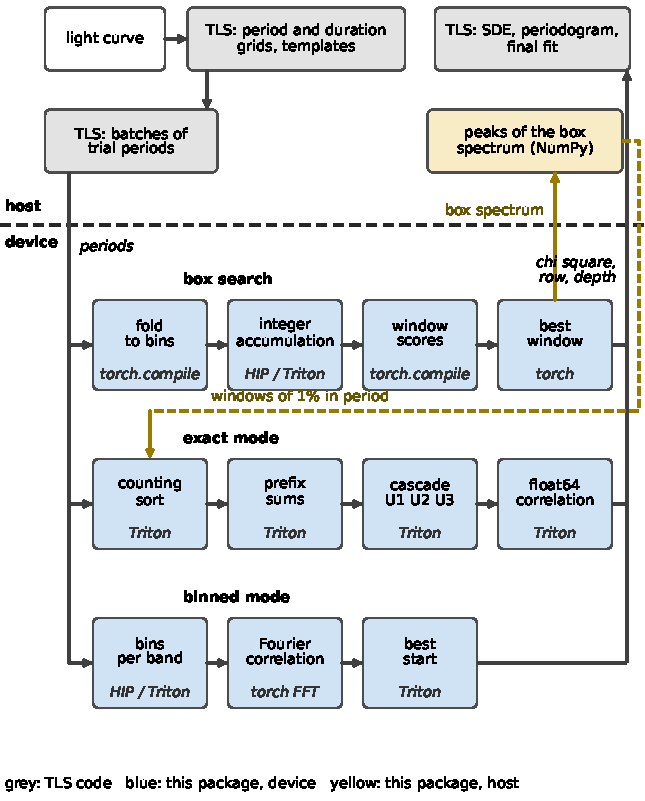
\includegraphics[width=0.62\textwidth]{pipeline.pdf}
\caption{The architecture of the package. Above the line, the host: the light curve, the period and duration grids and the templates of TLS, the loop over batches of trial periods, and the periodogram, the SDE and the final fit, grey where the code is TLS 2.0.1's. Below the line, the device: the three paths of a batch, the box search (the fold to bins, the integer accumulation, the window scores from cumulative sums), exact mode (the counting sort, the prefix sums, the cascade $U_1$, $U_2$, $U_3$, the float64 correlations of the survivors) and binned mode (the bins of each band, the Fourier correlation, the best start), with the code that runs each stage at its arrow (the HIP kernel on ROCm or the Triton kernel, Triton, \texttt{torch.compile}, the Fourier transform of torch). The hybrid search is the loop from the peaks of the box spectrum, found on the host, back into exact mode on narrow windows. The names are those of Sect.~\ref{sec:box} to \ref{sec:hybrid}.}\label{fig:pipeline}
\end{figure}

\FloatBarrier
\section{Data and methods}\label{sec:method}

\subsection{Characterization cases}\label{sec:cases}
TLS 2.0.1 ships 14 characterization cases: short runs on synthetic and K2 \citep{Howell2014} light curves with different grids, templates, errors and gaps. The two K2 light curves are EPIC 201367065 and EPIC 206154641. We run each case with TLS fused and with exact mode and compare the results field by field.

\subsection{Benchmark input}\label{sec:input}
The benchmark times every search on one input with one period grid. The light curve has $N=2\times10^4$, $10^5$ or $2\times10^5$ points evenly spaced over 1\,000 days, flat flux with Gaussian noise of 1\,000\,ppm, and one injected box with a period of 3.18\,d, a depth of 3\,000\,ppm and a duration of 2.5\,h, drawn from a fixed seed. The period grid is that of TLS from 0.5 to 14 days, with \NP{gpu}{200000} trial periods. The searches do different amounts of work per period: the box search scores about 24 durations on average, astropy's \texttt{BoxLeastSquares} one list of 37 durations, and TLS a template at 38 durations limited by the stellar limits at each period. For the search of many light curves, 64 light curves of $2\times10^4$ points are each given their own noise. Longer grids use 72\,000 points over 1\,500 days and 144\,000 points over 3\,000 days, with periods up to half the baseline; these are the sizes of the GTLS benchmark \citep{Hu2026}.

\subsection{Real TESS light curves}\label{sec:realstars}
The recovery of injected planets is measured on synthetic light curves (Sect.~\ref{sec:recovery}) and on one sector of the 2-minute PDCSAP light curve of each of 12 quiet TESS dwarfs, three each of F, G, K and M type by the effective temperature of the TESS Input Catalog (F 6\,000 to 7\,300\,K, G 5\,300 to 6\,000\,K, K 3\,900 to 5\,300\,K, M below 3\,900\,K) with $\log g$ of at least 4.0. A star was taken if it is not in the TOI table (snapshot of 2026-10-21), has CROWDSAP of at least 0.99, a TESS magnitude from 8.5 to 12, at least 17\,500 cadences with quality flag 0, and a 5-to-95 percent range of its flux binned to 0.5 days of at most twice what its white noise gives; the first three of each type that pass, in a seeded order, were taken. The 12 are from sectors 1, 2, 20, 21, 39, 41, 89 and 97, with TESS magnitudes from 8.6 to 12.0 and a white-noise scatter from 531 to 3\,167\,ppm; \texttt{validation/stars.json} lists each with its TIC number, sector, effective temperature, file and SHA-256, which \texttt{validation/fetch.py} downloads and verifies. The planets of Sect.~\ref{sec:recovery} are injected into each star, 3 at each of the 30 cells of period and signal to noise (1\,080 in all), and the light curve is then flattened with the same biweight filter as the synthetic classes. The injected transits are those of a planet around a star of the solar density on every star, as in the synthetic classes, and the duration grid is TLS's default for a solar star, so on the K and M dwarfs the durations are longer than those of a physical transit of theirs; the test measures the searches on real noise, not on physical durations. The errors given to every search on a real star are the median of the reported errors of its sector, so that binned mode, which needs equal errors, runs on the same input as the others; the real-star test therefore does not exercise per-point weights. The null set of each star is the star itself and 100 copies of it shuffled in blocks of one day after flattening.

\subsection{Per-star thresholds from block shuffles}\label{sec:thresholds}
The SDE of the box search is a z-score over the period grid of one light curve and has no threshold of its own. A threshold per light curve can be set by the largest SDE among $n$ copies of it, each shuffled in blocks within each sector; the block length and $n$ are parameters, and the defaults, used throughout this paper, are blocks of one day and $n=48$. The count sets the smallest false-alarm rate the threshold can resolve, $1/(n+1)$, and its cost, $n$ searches; 48 is the default because it resolves a rate of about 2\%, the rate at which the calibration of Sect.~\ref{sec:calibration} was tested, and no other value of $n$ is compared here. If the shuffled copies and a noise-only light curve are exchangeable, a noise search exceeds the threshold in 1 search in $n+1$, and the $k$-th largest SDE corresponds to a rate of $k/(n+1)$: at the default, 1 in 49 (2.04\%). The threshold is itself a random variable: the false-alarm probability of the threshold of one light curve follows a Beta$(1, n)$ distribution, at the default Beta$(1, 48)$, with a median of \Beta{median}\%, a 90th percentile of \Beta{p90}\% and a 99th percentile of \Beta{p99}\%, and the tail beyond 1 in 49 is not resolved. The box search folds a light curve and its shuffles together in one call; Sect.~\ref{sec:time} gives the cost, and Sect.~\ref{sec:calibration} tests the exchangeability on synthetic light curves and on 12 TESS stars.

A shuffled-block null keeps the structure inside a block and removes it between blocks, so the threshold guards against what survives that operation. \citet{Thompson2018} used inverted and scrambled light curves for Kepler and noted that inversion assumes false alarms that are symmetric under a flip of the flux. For TESS, \citet{Kunimoto2023FA} found pileups at aliases of the 13.7-day orbit in the BLS detections of 92\,899 M dwarfs and the same pileups in their inverted light curves, and \citet{Kunimoto2025LEO} built their false alarms by scrambling alone. Because the SDE is a z-score over the trial periods searched, it changes with the period range, and a threshold applies only to the grid on which it was made.

\subsection{Hardware and software}\label{sec:hardware}
All runs used an \Hw{cpu} with \Hw{logical_cpus} logical processors and an \Hw{gpu} (gfx1100) with \Hw{gpu_runtime}, under Python \Vs{python}, torch \Vs{torch}, NumPy \Vs{numpy}, Numba \Vs{numba}, astropy \Vs{astropy} and TLS \Vs{transitleastsquares}. The RX 7900 XTX is the consumer card of the Navi 31 die; the workstation card of the same die, the Radeon PRO W7900, has the same 96 compute units and boost clock of 2.50\,GHz, with 48\,GB of memory at 864\,GB/s in place of 24\,GB at 960\,GB/s \citep{GPUMonkey2026}. The package has been run only with ROCm on this GPU, not with CUDA.

\section{Results}\label{sec:results}

\subsection{Agreement of exact mode with TLS}\label{sec:correctness}
On each of the 14 characterization cases, exact mode agrees with TLS fused to within float64 rounding. The period grid, the duration grid, the number of transits and every integer field are identical, and the best period is the same grid point. Of the 41 result fields, 28 are identical in all cases; the other 13 differ in the last digits. Table~\ref{tab:validation} (Appendix~\ref{sec:appendix}) lists the 10 fields with the largest differences. The $\chi^2$ of every period differs by at most $1.8\times10^{-11}$ relative and the SDE by less than $10^{-11}$ (Table~\ref{tab:validation}; a rerun moves the last digit of these differences). The largest relative difference, $10^{-7}$ in the raw power, arises because the power divides by the spread of $\chi^2$, which amplifies its rounding by about $10^4$. In the tests, each component is checked against a reference implementation, and the screened search is checked against a brute-force search over all trial epochs.


\subsection{Adversarial cases}\label{sec:adversarial}
Eleven further light curves are built to stress the exact search, each compared with TLS fused: two planets of equal depth whose peaks nearly tie; the shortest templates of the grid (periods of 0.5 to 0.7\,d at 10-minute cadence) and the longest (periods of 20 to 45\,d over a baseline of 90\,d); time stamps that are duplicated and time stamps on a regular lattice, which tie in phase; the same light curve in BTJD and in BJD (an offset of 2\,459\,000\,d); errors that span five orders of magnitude and errors of $10^{-9}$ and $10^{3}$ among errors of $5\times10^{-4}$; a light curve of 40 points; and a light curve with 60\% of its baseline in gaps. The period and duration grids are equal in all eleven. The $\chi^2$ of every period agrees to at most \Adv{all}{chi2} relative over the eleven (the tests bound it at $10^{-6}$), and in ten of them, where the best period is the same, every other field of the results agrees to at most \Adv{all}{other} relative. In the light curve of 40 points two trial periods have $\chi^2$ that differ by \Adv{tiny_light_curve}{chi2} relative, and exact mode returns \Adv{tiny_light_curve}{periodgpu}\,d where TLS fused returns \Adv{tiny_light_curve}{periodtls}\,d: the agreement to float64 rounding holds for the $\chi^2$ of every period, and the best period can differ when two periods lie within rounding of each other. The BJD light curve gives the period of its BTJD twin to a relative $10^{-9}$ and not bit for bit, because the grid follows the span of the times, which BJD rounds at $10^{-10}$\,d.

\subsection{The box search against a continuous search}\label{sec:boxcheck}
In the tests, the box search agrees with a plain NumPy loop over the algorithm of Sect.~\ref{sec:box}, and on the light curves of the tests and the 200 trial periods of Table~\ref{tab:bins} (Appendix~\ref{sec:appendix}) it never scored above an exhaustive continuous box search over the same durations. Its power agreed bit for bit between a CPU and a GPU, across batch sizes and on repeated runs, except in one complete run of the test file, in which two batch sizes and a call with weights of one gave powers that differ by up to $1.3\times10^{-9}$ relative, with equal depths: after eight variants of the scoring function torch stops compiling it and runs further variants eagerly, which differs from the compiled scoring in the last digits, and two calls of one test can fall on either side of that limit. Its 32-bit scores give the same best period as 64-bit scores.

The box search differs from the continuous BLS statistic in three ways: it bins the phase, it quantizes the flux to $10^{-9}$, and it scores in 32-bit floats. Phase binning has the largest effect, because box edges must lie on bin edges. Table~\ref{tab:bins} measures it on 200 trial periods of Gaussian noise (5\,000 points over 400\,d), for at least 3 or 12 bins across the shortest duration and duration steps of 1.5 or 1.1. We rescore the box that the binned search finds without bins and divide by the best statistic over every trial epoch at a point and every duration on a grid of ratio 1.02. At the defaults of 12 bins and a step of 1.1, the box keeps a median of 0.93 of the continuous statistic, so it loses 7\%; at 3 bins and a step of 1.5 it keeps 0.80.


\subsection{Recovery of injected planets at a matched false-alarm rate}\label{sec:recovery}
Each search was run on 1\,200 light curves with an injected planet in each of three synthetic classes of one sector (27.4\,d at 2-minute cadence), and on 1\,000 light curves with nothing injected (\texttt{validation/run.py}). The classes are white noise of 1\,000\,ppm, red noise (700\,ppm of white noise and an Ornstein--Uhlenbeck process of 500\,ppm with a correlation time of 0.3\,d) and a variable star (700\,ppm of white noise and a rotation signal: a sinusoid of 3\,000\,ppm at a period drawn log-uniformly from 0.8 to 10\,d, with its first harmonic at 40 percent of the amplitude, at random phases). The red and variable light curves are divided by a biweight filter of 3\,d (wotan) after the planet is injected, the same filter for every search; white noise is not filtered. The planets have periods of 0.8, 1.6, 3.2, 6.4 and 12.8\,d, six target signal-to-noise ratios from 4 to 20 (against the noise at the transit duration for the red and variable classes; \citealt{Pont2006}), an impact parameter uniform from 0 to 0.9 and a random epoch. A search finds a planet when its best peak has a period within 1\% of the planet's and a transit time within half a duration of a transit, and an SDE at or above the threshold of its own SDE statistic: the 95th percentile of the SDE of the 1\,000 noise-only light curves of the same class. Peaks at a harmonic of the period are counted apart and are not found. The hybrid is run with 1, 5, 10 and 20 refined peaks, and it is counted as finding a planet when any of those peaks is at the planet's period and the SDE of the box spectrum is above the threshold: its share is that of a candidate list of $k$ peaks, not of one best peak, which is why it is never below the box search and can exceed exact mode. By the protocol of the validation, a hybrid whose paired lower bound falls more than 10 points below exact mode in any class is reported as candidate generation and not as a search, which its loss in the variable class makes it. Because the threshold is set for each search and class, the searches are compared at a false-alarm rate of 5\%, not at one SDE.

Figure~\ref{fig:completeness} gives the share found at each signal to noise, and Table~\ref{tab:recovery} the thresholds and the shares with their Wilson intervals. In white noise the box search differs from exact mode by \Pd{white}{box}{est} points (\Pd{white}{box}{low} to \Pd{white}{box}{high}, the score interval of \citealt{Tango1998} for paired shares, S/N of 8 and above), binned mode by \Pd{white}{binned}{est} (\Pd{white}{binned}{low} to \Pd{white}{binned}{high}) and the hybrid with 5 peaks by \Pd{white}{hybrid5}{est} (\Pd{white}{hybrid5}{low} to \Pd{white}{hybrid5}{high}). In red noise binned mode differs by \Pd{red}{binned}{est} (\Pd{red}{binned}{low} to \Pd{red}{binned}{high}), the box search by \Pd{red}{box}{est} (\Pd{red}{box}{low} to \Pd{red}{box}{high}) and the hybrid with 5 peaks by \Pd{red}{hybrid5}{est} (\Pd{red}{hybrid5}{low} to \Pd{red}{hybrid5}{high}). In the variable class the box search differs by \Pd{variable}{box}{est} (\Pd{variable}{box}{low} to \Pd{variable}{box}{high}), the hybrid with 5 peaks by \Pd{variable}{hybrid5}{est} (\Pd{variable}{hybrid5}{low} to \Pd{variable}{hybrid5}{high}) and binned mode by \Pd{variable}{binned}{est} (\Pd{variable}{binned}{low} to \Pd{variable}{binned}{high}). Refining 20 peaks in place of 5 changes the share found by the hybrid by at most \Pm{hybrid20from5} points in any class, pooled over the signal-to-noise ratios.

The loss of the box search in the variable class is that of its statistic, not of this implementation. On the 200 injected light curves of that class at a signal to noise of 8 and their 200 nulls (\texttt{validation/box\_variable.py}), each search again at the 95th percentile of its own nulls, astropy's \texttt{BoxLeastSquares} with the same periods and durations finds \Bv{astropy}{found} planets (\Bv{astropy}{share}\%, \Bv{astropy}{low} to \Bv{astropy}{high}) and the box search \Bv{box}{found} (\Bv{box}{share}\%), a paired difference of \Bvd{astropy-box}{est} points (\Bvd{astropy-box}{low} to \Bvd{astropy-box}{high}); exact mode finds \Bv{exact}{found} (\Bv{exact}{share}\%). The thresholds here come from 200 nulls, so these counts differ by one or two from those of Table~\ref{tab:recovery}, whose thresholds come from 1\,000. The box search's SDE is a plain z-score over the trial periods, and the spectrum of a light curve with a rotation signal carries a trend across them. With the running-median detrending that TLS applies to its own spectrum applied to the box spectrum, the same box statistic finds \Bv{detrended}{found} (\Bv{detrended}{share}\%, \Bv{detrended}{low} to \Bv{detrended}{high}), \Bvd{detrended-box}{est} points more than the plain box (\Bvd{detrended-box}{low} to \Bvd{detrended-box}{high}) and \Bvd{detrended-exact}{est} points fewer than exact mode (\Bvd{detrended-exact}{low} to \Bvd{detrended-exact}{high}). The detrending is not part of the box search as released, because its effect on the false-alarm rate of the per-star threshold of Sect.~\ref{sec:thresholds}, which the shuffles set on the undetrended spectrum, was not measured; the difference that remains between the detrended box and exact mode is not explained here. The loss in red noise was not tested the same way.

On the 12 real TESS stars of Sect.~\ref{sec:realstars}, with the threshold of each search at the 95th percentile of its own 1\,212 nulls, exact mode finds \Rr{exact}{8}\% of the \Rr{n}{planets} injected planets at a signal to noise of 8 (\Rr{exact}{8low} to \Rr{exact}{8high}) and \Rr{exact}{10}\% at 10 (\Rr{exact}{10low} to \Rr{exact}{10high}), and every search finds all of them at 14 and 20. The other three searches find shares within 1 point of exact mode's: against it, binned mode differs by \Pd{real}{binned}{est} points (\Pd{real}{binned}{low} to \Pd{real}{binned}{high}), the box search by \Pd{real}{box}{est} (\Pd{real}{box}{low} to \Pd{real}{box}{high}) and the hybrid with 5 peaks by \Pd{real}{hybrid5}{est} (\Pd{real}{hybrid5}{low} to \Pd{real}{hybrid5}{high}), each interval holding zero. These stars were chosen quiet, so the loss of the box search and the hybrid on the rotating star of the synthetic classes does not appear on them; Table~\ref{tab:recovery} gives their thresholds and shares.

Table~\ref{tab:period} gives the share found at each injected period, over every signal to noise from 4 to 20 of that period (240 planets per period in a synthetic class, 216 on the real stars). The largest difference between binned mode and exact mode in any cell is in the variable class at 3.2\,d, \Rp{variable}{binned}{3.2} against \Rp{variable}{exact}{3.2}\%; at 12.8\,d, where a sector holds one or two transits, binned mode finds \Rp{white}{binned}{12.8} against \Rp{white}{exact}{12.8}\% in white noise and \Rp{real}{binned}{12.8} against \Rp{real}{exact}{12.8}\% on the real stars. The box search loses nothing at 12.8\,d either (\Rp{white}{box}{12.8}\% in white noise, \Rp{real}{box}{12.8}\% on the real stars). Its loss is in the variable class at every period (\Rp{variable}{box}{0.8} against \Rp{variable}{exact}{0.8}\% at 0.8\,d, \Rp{variable}{box}{12.8} against \Rp{variable}{exact}{12.8}\% at 12.8\,d) and in red noise at short periods (\Rp{red}{box}{0.8} against \Rp{red}{exact}{0.8}\% at 0.8\,d, \Rp{red}{box}{12.8} against \Rp{red}{exact}{12.8}\% at 12.8\,d). The share found falls with period in white noise and on the real stars and rises with period in red noise and in the variable class; the cause of either shape is not measured here.

The comparison above is at one false-alarm rate. Figure~\ref{fig:roc} gives, for each class and for the real stars, the share of the injected planets found against the share of the noise-only light curves above the same SDE threshold, over every threshold (the true-positive rate against the false-positive rate, as \citealt{Hu2026} draw it for GTLS, TLS and BLS), with the planets at a signal to noise of 8 and above. At a false-positive rate of 1\%, exact mode finds \Roc{white}{exact}{0.01}\% in white noise, \Roc{red}{exact}{0.01}\% in red noise, \Roc{variable}{exact}{0.01}\% in the variable class and \Roc{real}{exact}{0.01}\% on the real stars, binned mode \Roc{white}{binned}{0.01}, \Roc{red}{binned}{0.01}, \Roc{variable}{binned}{0.01} and \Roc{real}{binned}{0.01}\%, and the box search \Roc{white}{box}{0.01}, \Roc{red}{box}{0.01}, \Roc{variable}{box}{0.01} and \Roc{real}{box}{0.01}\%. In white noise the four searches stay within about one point of each other at every rate from 1\% to 50\%. In red noise binned mode stays within one point of exact mode at every rate, while the box search and the hybrid fall further behind exact mode as the rate falls (\Roc{red}{box}{0.01} against \Roc{red}{exact}{0.01}\% at 1\%, \Roc{red}{box}{0.05} against \Roc{red}{exact}{0.05}\% at 5\%), so the comparison at 5\% understates their loss at a stricter rate. In the variable class the box search and the hybrid stay far below exact mode at every rate below 80\%, and the curves of binned and exact mode cross between 2\% and 2.5\%: binned mode is above exact mode at 1\% (\Roc{variable}{binned}{0.01} against \Roc{variable}{exact}{0.01}\%) and below it at 5\%. On the real stars the four searches are within a point of each other at 5\% and above, and at 1\% the box search and the hybrid are above exact mode (\Roc{real}{box}{0.01} against \Roc{real}{exact}{0.01}\%); below 1\% the threshold of 1\,212 nulls is set by a handful of them and the curves are not resolved. The order of the searches at 5\% therefore holds at 1\% in white and red noise and not in the variable class or on the real stars; why the box search leads on the real stars at 1\% is not measured here.

\begin{figure}[htbp]
\centering
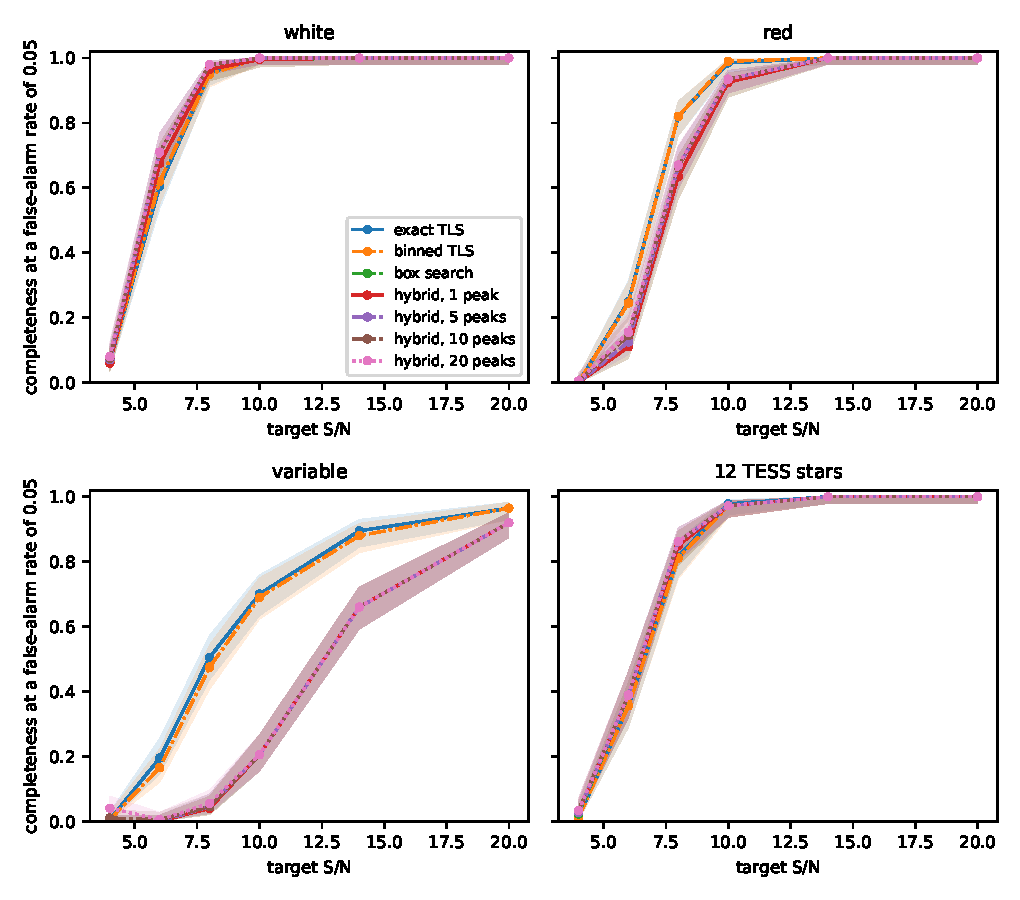
\includegraphics[width=0.8\textwidth]{completeness.pdf}
\caption{Share of the injected planets found at a false-alarm rate of 5\%, against the target signal to noise, in each noise class and on the 12 real TESS stars: every search, with its 95\% Wilson band. The bands of the exact and binned modes overlap.}\label{fig:completeness}
\end{figure}

\begin{figure}[htbp]
\centering
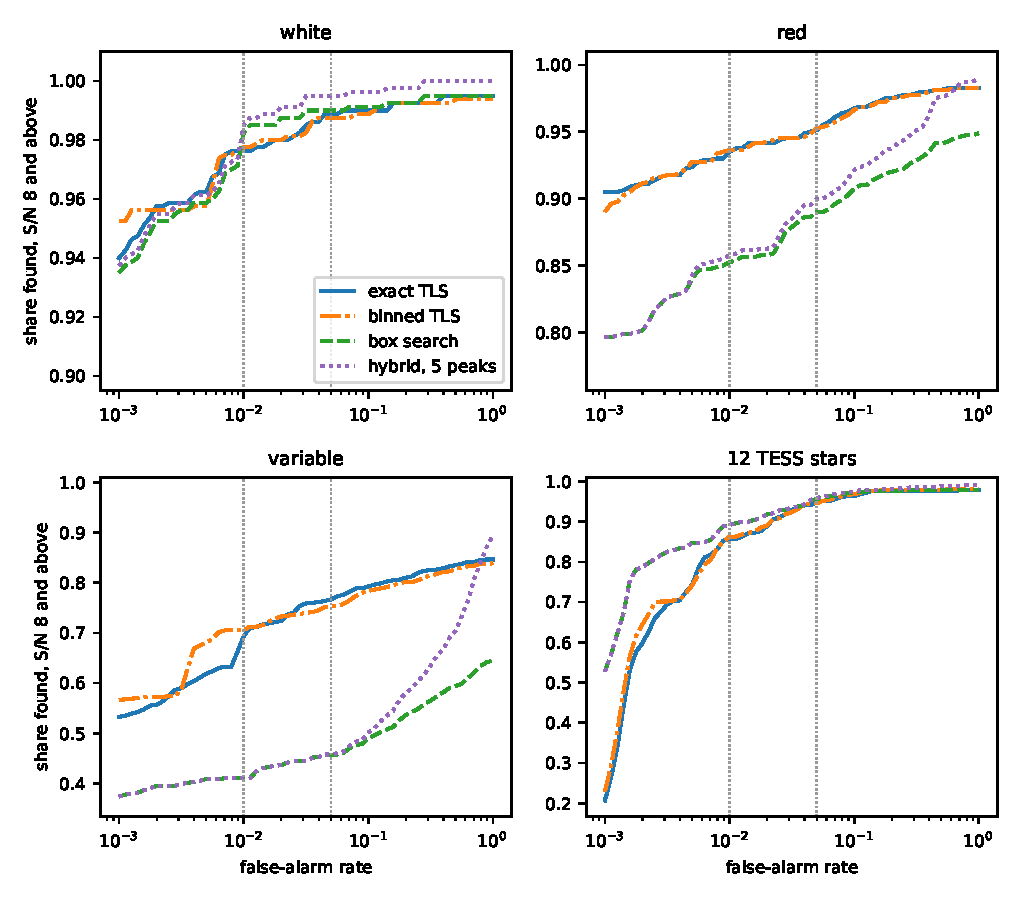
\includegraphics[width=0.8\textwidth]{roc.pdf}
\caption{True-positive rate against false-positive rate of the four searches over every SDE threshold, in each noise class and on the 12 real TESS stars, for the planets injected at a signal to noise of 8 and above against the noise-only light curves of the same class. The point at a false-positive rate of 5\% is the comparison of Table~\ref{tab:recovery}.}\label{fig:roc}
\end{figure}

\begin{table}[htbp]
\centering
\caption{Threshold of each search at a false-alarm rate of 5\% (SDE, with a bootstrap interval) and the share of injected planets found at target signal to noise of 6, 8 and 10, with the 95\% Wilson interval; 200 planets in each cell of the synthetic classes and 180 in each cell of the real stars.}\label{tab:recovery}
\footnotesize
\textbf{white noise}\\
% written by scripts/completeness.py
\begin{tabular}{lrrrr}
\toprule
search & threshold & S/N 6 & S/N 8 & S/N 10 \\
\midrule
exact & 7.5 (7.3 to 7.8) & 60\% (54 to 67) & 96\% (92 to 98) & 100\% (98 to 100) \\
binned & 7.6 (7.4 to 7.7) & 62\% (55 to 68) & 95\% (91 to 97) & 100\% (98 to 100) \\
box & 6.4 (6.3 to 6.6) & 68\% (61 to 74) & 96\% (93 to 98) & 100\% (97 to 100) \\
hybrid1 & 6.4 (6.3 to 6.6) & 68\% (61 to 74) & 96\% (93 to 98) & 100\% (97 to 100) \\
hybrid5 & 6.4 (6.3 to 6.6) & 71\% (64 to 77) & 98\% (95 to 99) & 100\% (98 to 100) \\
hybrid10 & 6.4 (6.3 to 6.6) & 71\% (64 to 77) & 98\% (95 to 99) & 100\% (98 to 100) \\
hybrid20 & 6.4 (6.3 to 6.6) & 71\% (64 to 77) & 98\% (95 to 99) & 100\% (98 to 100) \\
\bottomrule
\end{tabular}
\\[4pt]
\textbf{red noise}\\
% written by scripts/completeness.py
\begin{tabular}{lrrrr}
\toprule
search & threshold & S/N 6 & S/N 8 & S/N 10 \\
\midrule
exact & 7.5 (7.3 to 7.6) & 25\% (20 to 31) & 82\% (76 to 87) & 98\% (96 to 99) \\
binned & 7.5 (7.3 to 7.7) & 24\% (19 to 31) & 82\% (76 to 87) & 99\% (96 to 100) \\
box & 5.2 (5.1 to 5.2) & 11\% (7 to 16) & 64\% (57 to 70) & 92\% (88 to 95) \\
hybrid1 & 5.2 (5.1 to 5.2) & 11\% (7 to 16) & 64\% (57 to 70) & 92\% (88 to 95) \\
hybrid5 & 5.2 (5.1 to 5.2) & 12\% (9 to 18) & 66\% (60 to 73) & 94\% (89 to 96) \\
hybrid10 & 5.2 (5.1 to 5.2) & 14\% (10 to 20) & 66\% (60 to 73) & 94\% (89 to 96) \\
hybrid20 & 5.2 (5.1 to 5.2) & 16\% (11 to 21) & 67\% (60 to 73) & 94\% (89 to 96) \\
\bottomrule
\end{tabular}
\\[4pt]
\textbf{variable star}\\
% written by scripts/completeness.py
\begin{tabular}{lrrrr}
\toprule
search & threshold & S/N 6 & S/N 8 & S/N 10 \\
\midrule
exact & 9.2 (9.0 to 9.4) & 20\% (15 to 26) & 50\% (44 to 57) & 70\% (63 to 76) \\
binned & 9.2 (9.0 to 9.4) & 16\% (12 to 22) & 48\% (41 to 54) & 69\% (62 to 75) \\
box & 7.8 (7.7 to 7.9) & 0\% (0 to 2) & 4\% (2 to 8) & 20\% (15 to 27) \\
hybrid1 & 7.8 (7.7 to 7.9) & 0\% (0 to 2) & 4\% (2 to 8) & 20\% (15 to 27) \\
hybrid5 & 7.8 (7.7 to 7.9) & 0\% (0 to 2) & 4\% (2 to 8) & 20\% (15 to 27) \\
hybrid10 & 7.8 (7.7 to 7.9) & 0\% (0 to 3) & 4\% (2 to 8) & 20\% (15 to 27) \\
hybrid20 & 7.8 (7.7 to 7.9) & 0\% (0 to 3) & 6\% (3 to 10) & 20\% (15 to 27) \\
\bottomrule
\end{tabular}
\\[4pt]
\textbf{12 TESS stars}\\
\IfFileExists{recall_table_real.tex}{% written by scripts/completeness.py
\begin{tabular}{lrrrr}
\toprule
search & threshold & S/N 6 & S/N 8 & S/N 10 \\
\midrule
exact & 8.7 (8.4 to 9.1) & 36\% (29 to 43) & 82\% (75 to 87) & 98\% (94 to 99) \\
binned & 8.8 (8.4 to 9.1) & 36\% (29 to 43) & 81\% (75 to 86) & 97\% (94 to 99) \\
box & 6.8 (6.6 to 7.1) & 39\% (32 to 46) & 85\% (79 to 89) & 97\% (94 to 99) \\
hybrid1 & 6.8 (6.6 to 7.1) & 39\% (32 to 46) & 85\% (79 to 89) & 97\% (94 to 99) \\
hybrid5 & 6.8 (6.6 to 7.1) & 39\% (32 to 46) & 86\% (80 to 90) & 97\% (94 to 99) \\
hybrid10 & 6.8 (6.6 to 7.1) & 39\% (32 to 46) & 86\% (80 to 90) & 97\% (94 to 99) \\
hybrid20 & 6.8 (6.6 to 7.1) & 39\% (32 to 46) & 86\% (80 to 90) & 97\% (94 to 99) \\
\bottomrule
\end{tabular}
}{[\texttt{recall\_table\_real}]}
\end{table}

\begin{table}[htbp]
\centering
\caption{Share of the injected planets found at a false-alarm rate of 5\%, by injected period, over every signal to noise from 4 to 20 (240 planets per cell in the synthetic classes, 216 on the real stars), in percent with the 95\% Wilson interval.}\label{tab:period}
\footnotesize
% written by scripts/period_table.py
\begin{tabular}{lrrrrr}
\toprule
search & 0.8\,d & 1.6\,d & 3.2\,d & 6.4\,d & 12.8\,d \\
\midrule
\multicolumn{6}{l}{white noise} \\
exact & 80.8 (75.4--85.3) & 76.7 (70.9--81.6) & 78.3 (72.7--83.1) & 77.5 (71.8--82.3) & 72.1 (66.1--77.4) \\
binned & 80.8 (75.4--85.3) & 76.7 (70.9--81.6) & 78.3 (72.7--83.1) & 78.3 (72.7--83.1) & 72.1 (66.1--77.4) \\
box & 80.4 (74.9--84.9) & 77.9 (72.3--82.7) & 79.2 (73.6--83.8) & 79.6 (74.0--84.2) & 74.2 (68.3--79.3) \\
hybrid, 20 peaks & 82.5 (77.2--86.8) & 79.6 (74.0--84.2) & 79.6 (74.0--84.2) & 80.0 (74.5--84.6) & 75.8 (70.0--80.8) \\
\midrule
\multicolumn{6}{l}{red noise} \\
exact & 62.9 (56.6--68.8) & 66.7 (60.5--72.3) & 67.1 (60.9--72.7) & 70.0 (63.9--75.4) & 71.2 (65.2--76.6) \\
binned & 63.3 (57.1--69.2) & 66.7 (60.5--72.3) & 67.1 (60.9--72.7) & 69.6 (63.5--75.1) & 71.2 (65.2--76.6) \\
box & 49.2 (42.9--55.5) & 57.9 (51.6--64.0) & 62.9 (56.6--68.8) & 65.4 (59.2--71.1) & 70.4 (64.4--75.8) \\
hybrid, 20 peaks & 52.1 (45.8--58.3) & 59.2 (52.9--65.2) & 64.6 (58.3--70.4) & 66.7 (60.5--72.3) & 71.2 (65.2--76.6) \\
\midrule
\multicolumn{6}{l}{variable star} \\
exact & 43.3 (37.2--49.7) & 52.5 (46.2--58.7) & 57.1 (50.8--63.2) & 57.5 (51.2--63.6) & 61.7 (55.4--67.6) \\
binned & 42.1 (36.0--48.4) & 51.2 (45.0--57.5) & 55.0 (48.7--61.2) & 55.8 (49.5--62.0) & 60.8 (54.5--66.8) \\
box & 24.2 (19.2--30.0) & 22.9 (18.1--28.6) & 32.1 (26.5--38.2) & 35.4 (29.6--41.7) & 37.5 (31.6--43.8) \\
hybrid, 20 peaks & 25.8 (20.7--31.7) & 23.8 (18.8--29.5) & 32.9 (27.3--39.1) & 35.8 (30.0--42.1) & 38.8 (32.8--45.0) \\
\midrule
\multicolumn{6}{l}{real stars} \\
exact & 71.3 (64.9--76.9) & 72.2 (65.9--77.8) & 72.2 (65.9--77.8) & 68.5 (62.0--74.3) & 62.5 (55.9--68.7) \\
binned & 71.3 (64.9--76.9) & 71.8 (65.4--77.3) & 72.2 (65.9--77.8) & 68.5 (62.0--74.3) & 62.0 (55.4--68.2) \\
box & 72.7 (66.4--78.2) & 72.7 (66.4--78.2) & 72.7 (66.4--78.2) & 68.5 (62.0--74.3) & 66.2 (59.7--72.2) \\
hybrid, 20 peaks & 73.1 (66.9--78.6) & 73.1 (66.9--78.6) & 72.7 (66.4--78.2) & 69.0 (62.5--74.8) & 66.7 (60.1--72.6) \\
\bottomrule
\end{tabular}

\end{table}

\FloatBarrier
\subsection{Calibration of the shuffle threshold}\label{sec:calibration}
The threshold of Sect.~\ref{sec:thresholds} was tested on synthetic light curves of one flattened sector, 19\,740 points at 2-minute cadence, from the generator of the package (\texttt{validation/threshold.py}): 2\,000 noise-only light curves in each of three classes, searched with the box search from 0.5 to 14\,d together with 48 one-day block shuffles of each. The white class has white noise. The red class adds a correlated process to white noise, and the variable class adds a rotation signal. A second threshold comes from the same 48 shuffles of the inverted light curve (the flux reflected about its median). Table~\ref{tab:null} gives the share of light curves whose best peak exceeds the threshold. Figure~\ref{fig:nullsde} (Appendix~\ref{sec:appendix}) gives the distribution of the SDE of the noise-only light curves of each search in each class and on the real stars, with the thresholds at a false-alarm rate of 5\% of Table~\ref{tab:recovery} and the 48-shuffle thresholds of the box search beside them: in white and red noise the shuffle threshold of most light curves lies above the box search's 5\% threshold; in the variable class every shuffle threshold lies below it, which is the crossing of two thirds of the light curves in Table~\ref{tab:null}; on the real stars about half the stars' shuffle thresholds lie below it.

\begin{table}[htbp]
\centering
\caption{Share of noise-only light curves whose best peak exceeds the largest SDE of their 48 shuffles (the inverted light curve for the last column), with the 95\% Wilson interval in parentheses, against the nominal $1/49$.}\label{tab:null}
\small
% written by scripts/threshold_table.py
\begin{tabular}{lrrrrl}
\toprule
class & curves & above & shuffle threshold & nominal & inverted threshold \\
\midrule
white & 2\,000 & 50 & 2.5\% (1.9 to 3.3) & 2.0\% & 2.7\% (2.1 to 3.5) \\
red & 2\,000 & 16 & 0.8\% (0.5 to 1.3) & 2.0\% & 1.5\% (1.0 to 2.1) \\
variable & 2\,000 & 1\,325 & 66.2\% (64.1 to 68.3) & 2.0\% & 62.7\% (60.6 to 64.8) \\
\bottomrule
\end{tabular}

\end{table}

For white noise the share is \Th{white}{share}\% (\Th{white}{low} to \Th{white}{high}), which contains $1/49=2.04\%$. For red noise it is \Th{red}{share}\% (\Th{red}{low} to \Th{red}{high}): the threshold is conservative. We have not measured why; a candidate is the steps that the one-day blocks leave at their joints in flattened red noise (argued, not measured). For the variable class \Th{variable}{share}\% of the light curves cross. Of the \Vr{explained@of} crossings, \Vr{explained@count} (\Vr{explained@share}\%, \Vr{explained@low} to \Vr{explained@high}) have their best period at the rotation period or at its ratios 1/3, 1/2, 2 and 3, within 1\%. A shuffle in blocks of one day destroys periodicity, so this null treats a real periodic signal as a signal, and the share measures the strength of the rotation and not a false-alarm rate. The \Vr{unexplained@count} crossings left (\Vr{unexplained@share}\% of the light curves, \Vr{unexplained@low} to \Vr{unexplained@high}) are above $1/49$, and we do not call them noise. Of the \Vr{rest@of} variable light curves that do not cross, \Vr{rest@share}\% also peak at the rotation.

On the \Thr{n} real stars of Sect.~\ref{sec:realstars}, each searched with 199 shuffles, the test is whether the share of the shuffles that the star's own best peak outranks is uniform between 0 and 1, as exchangeability requires. The mean share is \Thr{mean}, and a Kolmogorov--Smirnov test against the uniform distribution gives \Thr{ks} with $p=\Thr{p}$, so exchangeability is not rejected on these stars; with \Thr{n} stars the test has little power, and the result does not make the threshold calibrated on real stars. Eight further stars of an earlier selection by the same rule, none in the list of Sect.~\ref{sec:realstars}, give a mean share of 0.677 and $p=0.12$; pooled, the \Thr{pooledn} stars give a mean of \Thr{pooledmean} and $p=\Thr{pooledp}$.

Planets were injected into the first light curves of each class, so that the same noise is searched with and without a planet (250 planets at each of six signal-to-noise ratios per class, the signal to noise of the red and variable classes taken against the noise at the transit duration; \citealt{Pont2006}). A planet is found when its best peak is at its period, within 1\% and half a duration of a transit, and above the largest SDE of its own 48 shuffles. Table~\ref{tab:injection} gives the shares: 87 to 92\% of the white-noise planets at a signal to noise of 10 to 20, 89 to 90\% of the red-noise planets at 14 to 20 and 84\% of the variable-class planets at 20. The best peak is at the injected period in 250 of 250 white-noise planets at each signal to noise from 10 to 20 and in 250 of 250 red-noise planets at 14 and 20 (247 of 250 at 10), and the planet raises its own threshold by a median factor of 1.3 to 1.6 at 14 to 20. The threshold of the inverted light curves finds 98.8 to 100\% of the white-noise planets at 10 to 20, 100\% of the red-noise planets at 14 and 20 (88.0\% at 10), and 83.2 to 96.8\% of the variable-class planets at 14 and 20.

\begin{table}[htbp]
\centering
\caption{Injected planets: the planets (250 in each row), those whose best peak is at the injected period (within 1\%), those at a harmonic, and the share found above the threshold of their own shuffles and of their inverted shuffles, with the 95\% Wilson interval.}\label{tab:injection}
\footnotesize
% written by scripts/threshold_table.py
\begin{tabular}{lrrrrll}
\toprule
class & S/N & planets & period & harmonic & above shuffle threshold & above inverted threshold \\
\midrule
white & 4 & 250 & 57 & 19 & 2.4\% (1.1 to 5.1) & 2.8\% (1.4 to 5.7) \\
white & 6 & 250 & 192 & 17 & 44.4\% (38.4 to 50.6) & 48.0\% (41.9 to 54.2) \\
white & 8 & 250 & 247 & 3 & 82.8\% (77.6 to 87.0) & 94.0\% (90.3 to 96.3) \\
white & 10 & 250 & 250 & 0 & 86.8\% (82.0 to 90.4) & 98.8\% (96.5 to 99.6) \\
white & 14 & 250 & 250 & 0 & 88.4\% (83.8 to 91.8) & 100.0\% (98.5 to 100.0) \\
white & 20 & 250 & 250 & 0 & 91.6\% (87.5 to 94.4) & 100.0\% (98.5 to 100.0) \\
red & 4 & 250 & 7 & 10 & 0.4\% (0.1 to 2.2) & 0.0\% (0.0 to 1.5) \\
red & 6 & 250 & 87 & 9 & 4.0\% (2.2 to 7.2) & 7.2\% (4.6 to 11.1) \\
red & 8 & 250 & 211 & 3 & 45.2\% (39.1 to 51.4) & 59.6\% (53.4 to 65.5) \\
red & 10 & 250 & 247 & 0 & 73.6\% (67.8 to 78.7) & 88.0\% (83.4 to 91.5) \\
red & 14 & 250 & 250 & 0 & 89.2\% (84.7 to 92.5) & 100.0\% (98.5 to 100.0) \\
red & 20 & 250 & 250 & 0 & 89.6\% (85.2 to 92.8) & 100.0\% (98.5 to 100.0) \\
variable & 4 & 250 & 1 & 6 & 0.4\% (0.1 to 2.2) & 0.4\% (0.1 to 2.2) \\
variable & 6 & 250 & 17 & 8 & 0.4\% (0.1 to 2.2) & 4.0\% (2.2 to 7.2) \\
variable & 8 & 250 & 73 & 10 & 11.2\% (7.9 to 15.7) & 19.2\% (14.8 to 24.5) \\
variable & 10 & 250 & 151 & 7 & 31.6\% (26.2 to 37.6) & 52.8\% (46.6 to 58.9) \\
variable & 14 & 250 & 217 & 0 & 65.6\% (59.5 to 71.2) & 83.2\% (78.1 to 87.3) \\
variable & 20 & 250 & 244 & 2 & 83.6\% (78.5 to 87.7) & 96.8\% (93.8 to 98.4) \\
\bottomrule
\end{tabular}

\end{table}

\FloatBarrier
\subsection{Run times}\label{sec:time}
Each timed call takes the times and fluxes on the host and returns its results on the host, so the GPU rows include the copies to and from the GPU and the final synchronization; Table~\ref{tab:timed} (Appendix~\ref{sec:appendix}) lists what each row includes. The box search is timed with the period grid given and does not fit the best period; the TLS rows and the rows of \texttt{transitgpu.tls} time the whole \texttt{power()} call, grids, template cache, spectra and final fit included; the hybrid row times the box search and one such call per peak; for astropy's \texttt{BoxLeastSquares}, the object is built before the timer starts. A call on 4\,000 points compiles the kernels before timing, and each time is the median of seven calls. That first call of a fresh process, on 4\,000 points, which the tables exclude, takes \Cold{gpu}{kept}\,s for the box search, \Cold{tls-gpu}{kept}\,s for exact mode, \Cold{tls-gpu-binned}{kept}\,s for binned mode and \Cold{hybrid}{kept}\,s for the hybrid when the compiled kernels are on disk from an earlier process; with those caches cleared, the call compiles them and takes \Cold{gpu}{cleared}\,s for the box search, \Cold{tls-gpu}{cleared}\,s for exact mode and \Cold{many}{cleared}\,s for the search of many light curves, which builds its HIP kernel with hipcc.


All rows were timed on one machine with one set of software versions, in one session on 2026-10-26, each as the median of seven calls, every part pinned to cores 0--15 on an otherwise idle machine with nothing else on the GPU. Table~\ref{tab:cpu} gives the times.

\begin{table}[htbp]
\centering
\caption{Time in seconds of one search over the period grid of TLS (\NP{gpu}{200000} trial periods from 0.5 to 14 days), as the median of seven calls. The box searches score a box and the others a template.}\label{tab:cpu}
\small
\begin{tabular}{lrrr}
\toprule
search & $2\times10^4$ points & $10^5$ points & $2\times10^5$ points \\
\midrule
transitgpu box search, GPU & \T{gpu}{20000} & \T{gpu}{100000} & \T{gpu}{200000} \\
\texttt{transitgpu.tls} exact mode, GPU & \T{tls-gpu}{20000} & \T{tls-gpu}{100000} & \T{tls-gpu}{200000} \\
\texttt{transitgpu.tls} binned mode, GPU & \T{tls-gpu-binned}{20000} & \T{tls-gpu-binned}{100000} & \T{tls-gpu-binned}{200000} \\
\texttt{transitgpu.tls} piecewise-linear mode (gpu-pl), GPU & \T{tls-gpu-pl}{20000} & \T{tls-gpu-pl}{100000} & \T{tls-gpu-pl}{200000} \\
hybrid search, 5 peaks, 1\% window, GPU & \T{hybrid}{20000} & \T{hybrid}{100000} & \T{hybrid}{200000} \\
astropy \texttt{BoxLeastSquares}, 1 thread & \T{astropy}{20000} & \T{astropy}{100000} & \T{astropy}{200000} \\
TLS fused-pl, 16 threads & \T{tls16}{20000} & \T{tls16}{100000} & \T{tls16}{200000} \\
TLS fused, 16 threads & \T{tls16-exact}{20000} & \T{tls16-exact}{100000} & \T{tls16-exact}{200000} \\
TLS fused-pl, 1 thread & \T{tls1}{20000} & \T{tls1}{100000} & \T{tls1}{200000} \\
TLS fused, 1 thread & \T{tls1-exact}{20000} & \T{tls1-exact}{100000} & \T{tls1-exact}{200000} \\
\bottomrule
\end{tabular}
\end{table}

At $2\times10^5$ points, exact mode takes \Ratio{tls16-exact}{tls-gpu}{200000} times less time than TLS fused on 16 threads and \Ratio{tls1-exact}{tls-gpu}{200000} times less than on one thread; binned mode takes \Ratio{tls16}{tls-gpu-binned}{200000} times less than TLS fused-pl on 16 threads, at the cost in accuracy given in Sect.~\ref{sec:binned}, and \Ratio{tls-gpu}{tls-gpu-binned}{200000} times less than exact mode. The box search takes \Ratio{astropy}{gpu}{200000} times less than astropy's \texttt{BoxLeastSquares} on one thread, which uses a different list of durations, and \Ratio{tls16}{gpu}{200000} times less than TLS fused-pl on 16 threads; the box search and TLS compute different statistics, so that ratio is not the speed-up of one algorithm.

The box search of 64 light curves of $2\times10^4$ points takes \T{many}{20000}\,s in one call; TLS fused-pl on 16 threads takes \T{tls16-many}{20000}\,s for the same light curves one after another. A threshold made from 48 shuffled copies of one light curve (Sect.~\ref{sec:thresholds}), the 48 copies searched in one call ($48\times$\NP{gpu}{20000} trial periods; the search of the light curve itself is a further search), takes \T{gpu-shuffles}{20000}, \T{gpu-shuffles}{100000} and \T{gpu-shuffles}{200000}\,s at the three sizes. With periods up to half the baseline, the box search takes \T{gpu}{72000}\,s for 72\,000 points over 1\,500 days (\NP{gpu}{72000} trial periods) and \T{gpu}{144000}\,s for 144\,000 points over 3\,000 days (\NP{gpu}{144000} trial periods).

\FloatBarrier
\subsection{Where the time goes}\label{sec:funnel}
The box search touches each point once per period and then scores a few hundred bins, so its time grows more slowly than the number of points: \T{gpu}{20000}\,s at $2\times10^4$ points and \T{gpu}{200000}\,s at $2\times10^5$. TLS fused-pl on 16 threads grows from \T{tls16}{20000}\,s to \T{tls16}{200000}\,s over the same range, so the ratio of the two grows from \Ratio{tls16}{gpu}{20000} to \Ratio{tls16}{gpu}{200000}.

Exact mode sorts the points of each period and screens the trial epochs. Table~\ref{tab:funnel} (Appendix~\ref{sec:appendix}) counts the trial epochs that survive each cascade bound for one batch of 64 periods in each of four period ranges at each size, as a share of those tested at the durations each period allows. Between 0.04\% and 0.47\% of trial epochs reach the exact correlation in every range and size, or 56 to 164 per period; $U_2$ removes most of what $U_1$ leaves, and $U_3$ most of what $U_2$ leaves. $U_1$ is most effective at long periods and small sizes: at $2\times10^4$ points and 5 to 14\,d it leaves 64\% of trial epochs, while at $2\times10^5$ points and 0.5 to 2\,d it leaves all of them. Counted by template length, the share that reaches the correlation exceeds 1\% only for the longest templates at each size, up to 2.77\% for templates of 2\,048 to 4\,095 samples at $2\times10^4$ points and 2 to 5\,d; these templates have both the most survivors and the most samples to sum.



Table~\ref{tab:split} (Appendix~\ref{sec:appendix}) splits the GPU time of exact mode over the whole grid by stage, from the profiler, with each kernel counted once. The fold, which sorts the points, grows with the number of points (\Sp{20000}{fold} to \Sp{200000}{fold}\,s), and so does the screening (\Sp{20000}{screening} to \Sp{200000}{screening}\,s), although the number of trial epochs tested in a batch of 64 periods barely changes with size ($2.4\times10^6$, $2.3\times10^6$ and $2.3\times10^6$ at 0.5 to 1\,d); we have not measured what causes that growth. The screening takes most of the time at $2\times10^4$ points, while at $2\times10^5$ the fold, the scans and the screening take similar shares. The profiler slows the run, and the host launches kernels while the GPU works, so these GPU times are not wall-clock times. Figure~\ref{fig:funnel} (Appendix~\ref{sec:appendix}) draws both tables.


\FloatBarrier
\subsection{Sanity check on WASP-18 b}\label{sec:wasp18}
This check shows that the searches run end to end on a real light curve with a known deep planet; it does not measure detection performance. We searched the first 13 days of the TESS 2-minute light curve of WASP-18 (TIC 100100827, sector 2; Figure~\ref{fig:wasp18}). The light curve is the Pre-search Data Conditioning Simple Aperture Photometry (PDCSAP) flux of the Science Processing Operations Center (SPOC; \citealt{Jenkins2016}), flattened with wotan \citep{Hippke2019wotan} using a biweight filter with a 0.75\,d window. Between 0.5 and 5 days, the box search finds a period of 0.94176\,d, a duration of 1.90\,h, a depth of 10\,086\,ppm and an SDE of 10.6. Exact mode finds the same period, a duration of 2.09\,h, a depth of 10\,915\,ppm and an SDE of 25.9. The NASA Exoplanet Archive \citep{Akeson2013} lists a period of 0.94145\,d for WASP-18 b \citep{Hellier2009}. The two SDEs are on different scales: that of the box search is a z-score of its statistic without detrending, and that of exact mode is a z-score of the TLS statistic after running-median detrending, so their ratio is not a ratio of significance.

\begin{figure}[htbp]
\centering
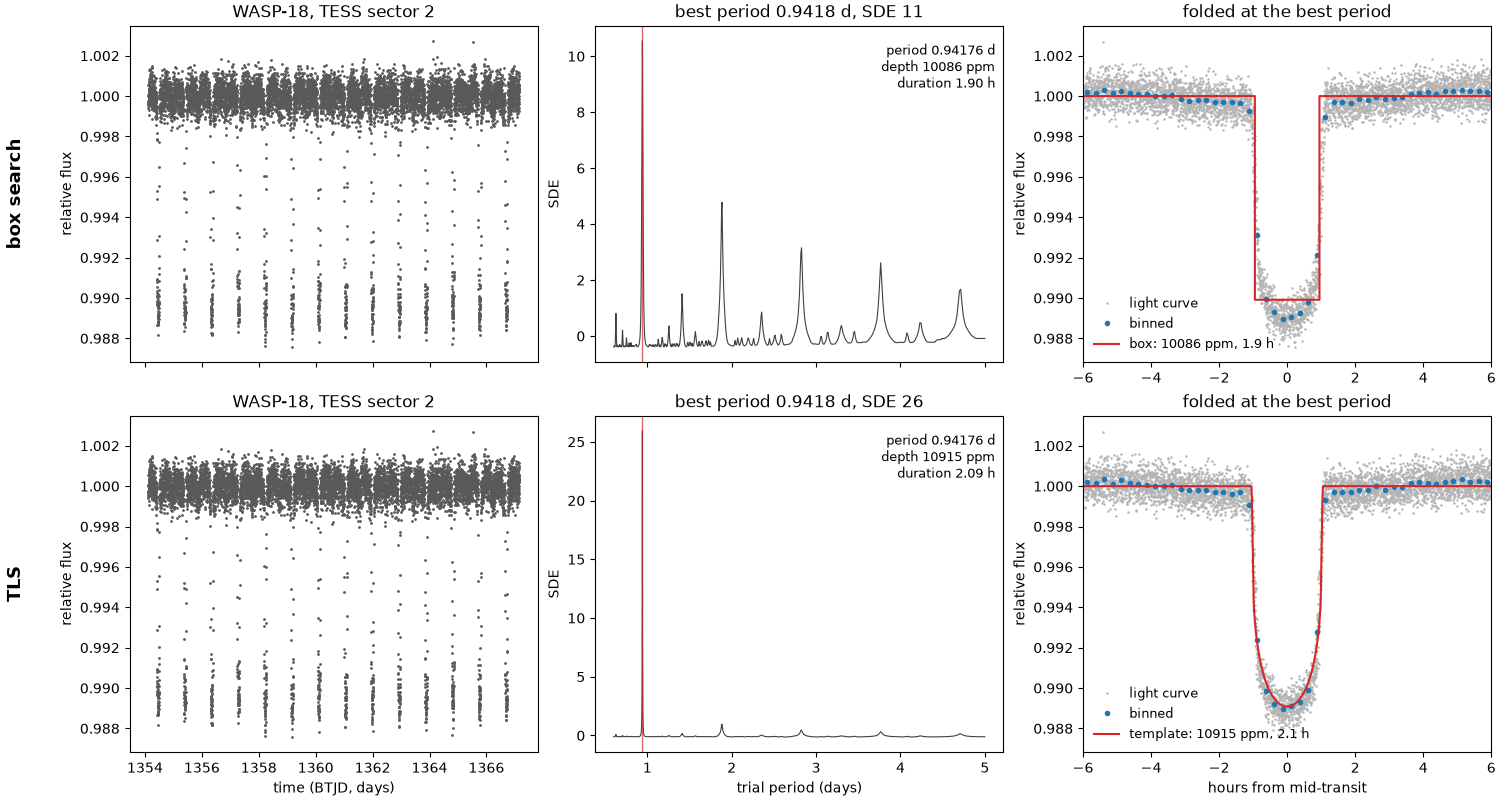
\includegraphics[width=\textwidth]{../docs/wasp18.png}
\caption{WASP-18 b in the first 13 days of TESS sector 2. Top: the box search; bottom: exact mode. Left: the flattened light curve. Middle: the SDE spectrum, with the best period marked. Right: the light curve folded at the best period, binned (blue), with the box or the template that was found (red).}\label{fig:wasp18}
\end{figure}

\FloatBarrier
\section{Comparison with GTLS}\label{sec:gtls}

\subsection{Design}\label{sec:gtlsdesign}
GTLS \citep{Hu2026} is the other port of TLS to a GPU. It is written with CuPy and CUDA kernels and needs an NVIDIA device. This section describes the paper of \citet{Hu2026} and the source of release 0.5.1 of its package (commit 74e449c of its public repository, 21 January 2026). Sect.~\ref{sec:exact} follows the data layout of release 0.4.4, every function of which exists in 0.5.1, three of them changed in the memory they reuse between batches of periods and one in a prefix sum of the squared residuals; the archive of 0.4.4 does not hold the CUDA kernel file, so the kernels were read in 0.5.1 only.

Table~\ref{tab:gtls} sets the steps of the two ports against TLS. Both keep the period grid of \citet{Ofir2014} as TLS builds it. The source of GTLS release 0.5.1 has the three duration constants of TLS 2.0.1 (stellar radii from $0.13$ to $3.5$ solar radii and a transit of at most $0.12$ of the period: \texttt{constants.py} and the kernel \texttt{durationsGrid} in \texttt{GPUFun.cu}, against \texttt{tls\_constants.py}), while the paper of GTLS describes wider limits, $T_{14}P^{-2/3}$ from $20.05$ to $620.84\,\mathrm{s}^{2/3}$ instead of the $41.39$ to $546.94\,\mathrm{s}^{2/3}$ that it derives for TLS, and a transit of at most $0.15$ of the period \citep[Sect.~2.2.2]{Hu2026}; we did not find these limits in the source that we read. GTLS folds in float64 and sorts with CuPy; the sort is not described as a stable sort of the float64 phases. Its search of the trial epochs $T_0$ has two stages \citep[Sect.~2.5]{Hu2026}: a shift every $0.125$ of the template width at every period (\texttt{T0\_FIT\_MARGIN} in \texttt{constants.py}), then every shift around the roughly 200 periods with the highest SDE. TLS 2.0.1 tests a shift every $0.01$ of the width at every period for templates wider than 100 cadences, and exact mode of \texttt{transitgpu.tls} tests the same shifts. GTLS computes the $\chi^2$ outside the transit by a recursion over $T_0$ and, as its authors write, approximates it by subtracting the mean flux in the transit from unity and squaring the result \citep[Sect.~2.3.4]{Hu2026}; the term inside the transit is a direct sum. In its source the times, the periods and the fold are float64, and the flux, the errors, the sums of the $\chi^2$ and the best $\chi^2$ of each period are float32 (\texttt{core.py}; the kernels \texttt{foldFast}, \texttt{calcAllFullSum} and \texttt{calcAllOutOfTransitResiduals} in \texttt{GPUFun.cu}). The exact backend of TLS 2.0.1 works in float64, its float32 storage belonging to its approximate backends, and exact mode of \texttt{transitgpu.tls} works in float64 throughout. We do not measure here what the difference does to the result of GTLS or to its speed.

\begin{table}[htbp]
\centering
\caption{The steps of TLS 2.0.1, of GTLS (paper of \citealt{Hu2026} and release 0.5.1) and of exact mode of \texttt{transitgpu.tls}.}\label{tab:gtls}
\small
\begin{tabular}{R{2.2cm}R{3.4cm}R{4.2cm}R{4.2cm}}
\toprule
 & TLS 2.0.1 & GTLS & \texttt{transitgpu.tls}, exact mode \\
\midrule
period grid & \citet{Ofir2014} & the same procedure, longest period half the span & TLS code \\
duration grid & stellar radii $0.13$ to $3.5$, at most $0.12$ of the period & the same constants in the source; the paper describes $20.05$ to $620.84\,\mathrm{s}^{2/3}$ and at most $0.15$ & TLS code \\
fold and sort & float64 phase, sort by phase & float64 phase $t/P-\lfloor t/P\rfloor$, CuPy sort & the permutation of a stable float64 sort \\
trial epochs & every $0.01$ of the width for templates wider than 100 cadences & stage 1: every $0.125$ of the width; stage 2: every shift, for about 200 periods & those that TLS tests \\
$\chi^2$ & exact & outside the transit approximated, inside a direct sum & exact for the trial epochs that pass the bounds \\
precision & float64 & times, periods and fold float64; flux, errors, $\chi^2$ sums and best $\chi^2$ float32 & float64 throughout \\
SDE & from $\chi^2$, detrended & from $\chi^2$, detrended \citep[Sect.~2.4]{Hu2026} & TLS code \\
\bottomrule
\end{tabular}
\end{table}

\subsection{Exactness}\label{sec:gtlsexact}
Exact mode reproduces the $\chi^2$ of TLS fused at every trial period: it agrees to at most $1.8\times10^{-11}$ relative on the 14 characterization cases of TLS and to at most \Adv{all}{chi2} on the adversarial cases (Sects.~\ref{sec:correctness} and \ref{sec:adversarial}). Its grids, statistics and final fit are those of TLS. GTLS departs from the $\chi^2$ of TLS in three ways that its authors state or that its source shows: the first stage tests a coarser set of trial epochs, the arrays are float32, and the term outside the transit is approximated. Its search space may also differ: the paper describes a wider range of durations than that of TLS, which the source that we read does not show. A $\chi^2$ taken over a subset of the trial epochs of the same durations is not lower than the minimum over all of them, so the $\chi^2$ of GTLS at a period that is not among the refined candidates is a minimum over fewer shifts than that of TLS.

The authors report, on synthetic light curves of four years at 30-minute cadence with 110\,ppm of white noise and injected Earth-sized transits, a precision of $9.3\%$ and a recall of $79.4\%$ for GTLS and $9.4\%$ and $81.1\%$ for TLS, with the thresholds SDE $=7$ and SNR $=5$, and call them statistically consistent \citep[Table~1]{Hu2026}. If both searches ran on one set of light curves with these thresholds, an exact port gives the SDE and the SNR of TLS, so it makes the same decisions on every light curve and has the same precision and the same recall. A recall $1.7$ points lower therefore means that the statistic of GTLS differs from that of TLS on some of the light curves. It does not say which difference causes this (the coarse trial epochs, the float32 arrays, the approximation or, if the paper's wider range of durations is used, the durations), and it does not say that GTLS is worse. No run of GTLS was obtained here (Sect.~\ref{sec:gtlstime}), so the comparison of this section is one of design.

\subsection{Run times}\label{sec:gtlstime}
On light curves of the size of those of the GTLS paper (30-minute cadence, 1\,500 and 3\,000 days, \NP{tls-gpu}{72000} and \NP{tls-gpu}{144000} trial periods from the grid of TLS to half the baseline), TLS 2.0.1 on 16 threads takes \T{tls16-exact}{72000}\,s and \T{tls16-exact}{144000}\,s, exact mode of \texttt{transitgpu.tls} \T{tls-gpu}{72000}\,s and \T{tls-gpu}{144000}\,s, and binned mode \T{tls-gpu-binned}{72000}\,s and \T{tls-gpu-binned}{144000}\,s. % the rows tls16-exact, tls-gpu and tls-gpu-binned at the sizes 72000 and 144000 come from the session of results.json; the text is checked against the file before it is merged
These rows were timed in the session of Table~\ref{tab:cpu}, on the machine of Sect.~\ref{sec:hardware}, with float64 and the margin of $T_0$ of $0.01$ of TLS. At the margin of $0.125$ of GTLS, TLS on 16 threads takes \T{tls16-exact-margin}{72000}\,s and \T{tls16-exact-margin}{144000}\,s, and exact mode \T{tls-gpu-margin}{72000}\,s and \T{tls-gpu-margin}{144000}\,s (Table~\ref{tab:gtlstimes}).

The paper of GTLS times its search on light curves made with batman at 30-minute cadence over about 1\,500 and 3\,000 days, on an NVIDIA RTX 4090, and TLS on an AMD Ryzen 9 7950X: \Gt{time}{72000}\,s for GTLS against \Gt{tls}{72000}\,s for TLS at 1\,500 days, and \Gt{time}{144000}\,s against \Gt{tls}{144000}\,s at 3\,000 days, with 79\,s on two GPUs \citep[Sect.~3.4]{Hu2026}. That section does not state the noise, the planet, the thread count of TLS, the number of calls or the margin of $T_0$ of its timings; the default of its source is $0.125$, and its Sect.~4.2 reports that lowering the margin from $0.1$ to $0.01$ raises the run time of GTLS by about 37\% and that of TLS by about 8\%.

The two GPUs are consumer cards of the same year, 2022, with the published and the attained figures of Table~\ref{tab:hardware}. The published peaks are the manufacturers' where their documents state them and a specification database's otherwise, as the table says; the attained column is what \texttt{benchmarks/peak.py} reaches on the GPU used here with a Triton kernel of independent fused multiply-adds and a copy of 2\,GiB, a lower bound on the peak, measured with the device otherwise idle. Table~\ref{tab:gtlstimes} sets the published times of GTLS beside the times measured here on light curves of the same length and cadence. The ratio in its last column is a comparison across two machines, two sets of light curves and two implementations that return different results, not the speed-up of one search on one machine: at the margin of GTLS, exact mode takes \Gt{ratio}{72000} times less than the published time of GTLS at 1\,500 days and \Gt{ratio}{144000} times less at 3\,000 days, and returns the $\chi^2$ of TLS. The TLS run of the GTLS paper took \Gt{tlsratio}{72000} and \Gt{tlsratio}{144000} times longer than TLS fused on 16 threads here at the margin of 0.125, which shows how far the two papers' baselines differ in hardware, version and settings before any search is compared.

\begin{table}[htbp]
\centering
\caption{The GPU of the GTLS paper and the GPU used here. Published: the manufacturer's figure where its document states it (NVIDIA's Ada whitepaper, \citealt{NVIDIA2022Ada}, and product page, \citealt{NVIDIA4090}; AMD's product support page, \citealt{AMD7900XTX}, for the compute units and the clock), otherwise a specification database (\citealt{Notebookcheck7900XTX}), each named in the cell. Attained: \texttt{benchmarks/peak.py} on the GPU used here, at a shader clock of up to \Pk{clockmax}\,MHz. The FP64 figure of the RTX 4090 follows from the whitepaper's statement that its FP64 rate is 1/64 of its FP32 rate; the FP32 figure of the RX 7900 XTX counts dual-issue, and the FP64 figure of the database is that figure over 32.}\label{tab:hardware}
\small
\begin{tabular}{R{3.2cm}R{4.6cm}R{6.2cm}}
\toprule
 & NVIDIA RTX 4090 (GTLS paper) & AMD RX 7900 XTX (this paper) \\
\midrule
memory & 24\,GB GDDR6X, 384-bit (product page) & 24\,GB GDDR6, 384-bit (database) \\
cores and clock & 16\,384 CUDA cores, boost 2.52\,GHz (product page) & 96 compute units, boost 2.50\,GHz (support page) \\
memory bandwidth, published & 1\,008\,GB/s (whitepaper) & 960\,GB/s (database) \\
memory bandwidth, attained & not measured & \Pk{copy}\,GB/s (\Pk{copyshare}\% of the published) \\
FP32, published & 82.6\,TFLOPS (whitepaper) & 61.4\,TFLOPS with dual-issue (database) \\
FP32, attained & not measured & \Pk{fp32}\,TFLOPS, single-issue \\
FP64, published & 1.29\,TFLOPS (1/64 of FP32) & 1.9\,TFLOPS (database, 61.4/32) \\
FP64, attained & not measured & \Pk{fp64}\,TFLOPS (1/\Pk{ratio} of the attained FP32) \\
\bottomrule
\end{tabular}
\end{table}

\begin{table}[htbp]
\centering
\caption{Run times on light curves of the length and cadence of the GTLS benchmark (30-minute cadence; \NP{tls-gpu}{72000} and \NP{tls-gpu}{144000} trial periods here), in seconds. Ours: the session of Table~\ref{tab:cpu}, the median of seven calls, float64, on the GPU of Table~\ref{tab:hardware}. GTLS: the times its paper publishes for its own light curves on an RTX 4090 \citep[Sect.~3.4]{Hu2026}, with float32 sums, at a margin of $T_0$ the paper does not state (its source's default is $0.125$). The last column divides the published time of GTLS by the time of exact mode at the margin of $0.125$: a comparison across two machines, two sets of light curves and two statistics.}\label{tab:gtlstimes}
\small
\begin{tabular}{lrrrrrr}
\toprule
 & TLS fused, 16 threads & exact mode & TLS fused, 16 threads & exact mode & GTLS, published & ratio \\
 & margin 0.01 & margin 0.01 & margin 0.125 & margin 0.125 & & \\
\midrule
1\,500 days & \T{tls16-exact}{72000} & \T{tls-gpu}{72000} & \T{tls16-exact-margin}{72000} & \T{tls-gpu-margin}{72000} & \Gt{time}{72000} & \Gt{ratio}{72000} \\
3\,000 days & \T{tls16-exact}{144000} & \T{tls-gpu}{144000} & \T{tls16-exact-margin}{144000} & \T{tls-gpu-margin}{144000} & \Gt{time}{144000} & \Gt{ratio}{144000} \\
\bottomrule
\end{tabular}
\end{table}
A run of GTLS release 0.4.4 through the ROCm build of CuPy on this GPU, with a module in the run script answering GTLS's three calls to NVIDIA's management library with the free memory that the HIP runtime reports, gave a finite $\chi^2$ at fewer than 3\% of the trial periods, with values that varied between runs; the cause was not identified. No time of GTLS was measured here, and nothing in this paper is a statement about GTLS on the hardware it was written for.

\FloatBarrier
\section{Discussion}\label{sec:discussion}
The searches trade accuracy against run time, and the measurements of Sect.~\ref{sec:recovery} say where each trade is safe. Binned mode is the fastest of the searches whose recovery is within \Pm{binned} points of exact mode in every class at a matched false-alarm rate, in \Ratio{tls-gpu}{tls-gpu-binned}{200000} times less time than exact mode; it departs from TLS in $\chi^2$ where the phase coverage is uneven (Table~\ref{tab:binned}), but not in recovery on these light curves. The box search and the hybrid find as many planets as exact mode in white noise, within 1 point, and on the 12 quiet TESS stars, where every interval holds zero, so on such stars the measurements do not separate the four searches and the choice is one of run time; they serve as a faster first pass, with exact TLS for confirmation. In correlated noise they find \Pd{red}{hybrid5}{round} to \Pd{red}{box}{round} points fewer and on a rotating star \Pd{variable}{box}{round} points fewer, so binned or exact mode should be used there. The hybrid evaluates the TLS statistic only near the five highest peaks of the box spectrum, and refining 20 peaks in place of 5 changes its share by at most \Pm{hybrid20from5} points, pooled over the signal-to-noise ratios; its losses are the box search's, since the SDE of each peak is the box search's. In the variable class the cause is measured: that SDE is a z-score of a spectrum that carries the trend of the rotation, which TLS's detrending removes; in red noise it was not measured.

The ratio of the time of TLS fused on 16 threads to the time of exact mode is \Ratio{tls16-exact}{tls-gpu}{20000}, \Ratio{tls16-exact}{tls-gpu}{100000} and \Ratio{tls16-exact}{tls-gpu}{200000} at the three sizes of Table~\ref{tab:cpu}, and \Ratio{tls16-exact}{tls-gpu}{72000} and \Ratio{tls16-exact}{tls-gpu}{144000} on the two longer light curves of Sect.~\ref{sec:gtlstime}, so it does not grow with the number of points. The share of trial epochs that reach the exact correlation stays below 0.5\% of those tested in every period range and size (Table~\ref{tab:funnel}; counted by template length, it reaches 2.8\% for the longest templates, Sect.~\ref{sec:funnel}), and the fold and the screening take more of the time of exact mode than the correlations do (Table~\ref{tab:split}). The tables do not separate the gain of the screening from the GPU's parallelism, and no measurement here does.

Against the searches named in the introduction, transitgpu differs in two ways. cuvarbase, GTLS and CETRA each need an NVIDIA GPU, whereas transitgpu runs through PyTorch and Triton and was run here on an AMD GPU with ROCm; it has not been run on NVIDIA hardware. Of the three, only GTLS ports TLS, and the TLS search of transitgpu keeps the TLS interface and results objects. Whether the shuffles in one launch make per-star thresholds practical for a survey depends on the calibration of Sect.~\ref{sec:calibration}, made on synthetic light curves of one sector: calibrated for white noise, conservative for the red noise of the generator, and on a variable star a flag of the rotation, which shuffles in blocks of one day cannot reproduce.

The comparison with GTLS (Sect.~\ref{sec:gtls}) is one of design and of published times: exact mode reproduces the $\chi^2$ of TLS where GTLS departs from it by design, the ratio of Table~\ref{tab:gtlstimes} is a comparison across machines, light curves and statistics, and none of the searches of this paper was compared with GTLS on injected planets.

\section{Conclusions}\label{sec:summary}
The box search searches a light curve of $2\times10^5$ points and 48 shuffled copies of it in one call in \T{gpu-shuffles}{200000}\,s, less than one search with TLS fused on 16 threads (Sect.~\ref{sec:time}), and its bin sums do not depend on the order of the additions (Sect.~\ref{sec:box}). Binned mode takes \T{tls-gpu-binned}{200000}\,s, \Ratio{tls16}{tls-gpu-binned}{200000} times less than TLS fused-pl on 16 threads, the backend whose statistic it approximates, and \Ratio{tls16-exact}{tls-gpu-binned}{200000} times less than TLS fused, and finds injected planets within \Pm{binned} points of exact mode in every class at a matched false-alarm rate (Sect.~\ref{sec:recovery}). Exact mode reproduces the $\chi^2$ of TLS fused to float64 rounding (Sects.~\ref{sec:correctness} and \ref{sec:adversarial}) and takes \T{tls-gpu}{200000}\,s, \Ratio{tls16-exact}{tls-gpu}{200000} times less than TLS fused on 16 threads, a ratio that does not grow with the number of points (Sect.~\ref{sec:discussion}). The hybrid search, at its default of five peaks, takes \T{hybrid}{200000}\,s and finds as many planets as exact mode in white noise and on quiet TESS stars, and fewer in correlated noise and on a rotating star (Sect.~\ref{sec:recovery}). The threshold from 48 block-shuffled copies is calibrated in white noise, conservative in red noise, and marks the rotation of a variable star as signal (Sect.~\ref{sec:calibration}). GTLS, an earlier CUDA port of TLS, approximates the TLS statistic with float32 sums and a coarse first pass over the trial epochs; exact mode reproduces it, and on light curves of the GTLS benchmark at the trial-epoch step of GTLS it takes \T{tls-gpu-margin}{72000} and \T{tls-gpu-margin}{144000}\,s on the RX 7900 XTX, where GTLS reports \Gt{time}{72000} and \Gt{time}{144000}\,s on an NVIDIA RTX 4090 (Sect.~\ref{sec:gtls}).

These results have limits. The recovery is measured on synthetic light curves of one sector and on one sector of each of 12 real TESS stars chosen quiet, at one cadence; stars with rotation or other variability, and longer baselines, were not tested with real data, and the transits injected into the real stars have the durations of a solar-density star on every star. The hybrid search is a way to generate candidates, scored by any of its refined peaks, and not a search scored by its best peak. The cause of the conservative threshold of the red class is not measured, and the loss that remains between the detrended box search and exact mode in the variable class is not explained. The package has been run only with ROCm on one AMD GPU; on other devices it uses only its Triton kernels, which Triton also compiles for NVIDIA GPUs, and its one HIP kernel, a faster accumulation of the box search, uses no AMD-specific instruction, but neither the speed nor the results on NVIDIA hardware have been measured. Every search here, as TLS and GTLS, folds at a strict ephemeris, so a planet whose transit times vary (transit timing variations) is folded out of alignment and its signal is lowered; none of the recovery tests injects such a planet. The package runs on one device: a call searches on one GPU, and the search of many light curves is one launch, not a division of the work across devices. All timings come from one machine and one strong, evenly sampled signal (3\,000\,ppm in 1\,000\,ppm of white noise), the screening statistics from one batch of periods per range, and a time ratio between the box search and TLS is not the speed-up of one algorithm, since they compute different statistics.

\section*{Software availability}
transitgpu 0.1.0 is available at \url{https://github.com/mauri870/transitgpu} under the MIT licence. The repository holds the tests, the benchmark script (\texttt{benchmarks/bench.py}), the examples, and the scripts that produce the numbers and tables of this paper (\texttt{paper/scripts}). The period- and duration-grid code that the package copies from TLS is under the MIT licence of TLS (Hippke and Heller).

\software{transitgpu 0.1.0, Python \Vs{python}, PyTorch \Vs{torch} \citep{Paszke2019}, Triton \Vs{triton} \citep{Tillet2019}, \Hw{gpu_runtime}, NumPy \Vs{numpy} \citep{Harris2020}, Numba \Vs{numba} \citep{Lam2015}, transitleastsquares \Vs{transitleastsquares} \citep{HippkeHeller2019}, astropy \Vs{astropy} \citep{Astropy2013,Astropy2018,Astropy2022}, batman \Vs{batman} \citep{Kreidberg2015}, wotan \Vs{wotan} \citep{Hippke2019wotan}}

\begin{acknowledgments}
An AI assistant helped with parts of the code and the writing; we reviewed all of it.
This paper includes data collected by the TESS mission. Funding for the TESS mission is provided by the NASA Science Mission Directorate. The data were obtained from the Mikulski Archive for Space Telescopes (MAST) at the Space Telescope Science Institute (STScI), which is operated by the Association of Universities for Research in Astronomy, Inc., under NASA contract NAS 5-26555. The TESS light curves are at MAST, doi:10.17909/t9-nmc8-f686.
This paper includes data collected by the K2 mission. Funding for the K2 mission is provided by the NASA Science Mission Directorate. STScI is operated by the Association of Universities for Research in Astronomy, Inc., under NASA contract NAS 5-26555.
This research has made use of the NASA Exoplanet Archive, which is operated by the California Institute of Technology, under contract with the National Aeronautics and Space Administration under the Exoplanet Exploration Program.
\end{acknowledgments}

\appendix
\section{Tables and figures of the validation and the timing}\label{sec:appendix}
Table~\ref{tab:binned} gives the best period and SDE of binned mode and of TLS fused-pl against TLS fused on the 14 characterization cases (Sect.~\ref{sec:binned}); Table~\ref{tab:validation} lists the fields of the results of TLS with the largest differences between exact mode and TLS fused on the 14 characterization cases (Sect.~\ref{sec:correctness}); Table~\ref{tab:bins} the share of the continuous box statistic that the box search keeps (Sect.~\ref{sec:boxcheck}); Table~\ref{tab:timed} what each timed row of Table~\ref{tab:cpu} includes (Sect.~\ref{sec:time}); Table~\ref{tab:funnel} the trial epochs that survive each bound of the screening cascade and Table~\ref{tab:split} the GPU time of exact mode by stage (Sect.~\ref{sec:funnel}). Figure~\ref{fig:nullsde} pictures the calibration of Sect.~\ref{sec:calibration} and Figure~\ref{fig:funnel} the two tables of Sect.~\ref{sec:funnel}.

\begin{table}[htbp]
\centering
\caption{Best period and SDE of TLS binned and TLS fused-pl against TLS fused on the 14 characterization cases.}\label{tab:binned}
\small
% written by scripts/binned_accuracy.py: 14 cases
\begin{tabular}{lcrcr}
\toprule
case & binned period & binned $|\Delta\mathrm{SDE}|$ & fused-pl period & fused-pl $|\Delta\mathrm{SDE}|$ \\
\midrule
\texttt{syn\_earth} & same & 0.022 & same & 0.001 \\
\texttt{syn\_earth\_gap} & different & 0.224 & same & 0.006 \\
\texttt{syn\_earth\_dy} & \multicolumn{2}{c}{unequal errors, refused} & same & 0.004 \\
\texttt{no\_fit} & same & 0.000 & same & 0.000 \\
\texttt{k2\_box} & same & 0.615 & same & 0.006 \\
\texttt{k2\_grazing} & same & 0.658 & same & 0.047 \\
\texttt{k2\_3\_window} & same & 0.870 & same & 0.000 \\
\texttt{k2\_3\_threads1} & same & 0.245 & same & 0.000 \\
\texttt{short\_lc} & different & 0.209 & same & 0.000 \\
\texttt{centered\_time} & same & 0.139 & same & 0.008 \\
\texttt{custom\_nonlinear} & same & 0.172 & same & 0.007 \\
\texttt{custom\_ecc\_squareroot} & same & 0.179 & same & 0.011 \\
\texttt{narrow\_stellar} & \multicolumn{2}{c}{unequal errors, refused} & same & 0.065 \\
\texttt{plato\_25s\_window} & same & 0.003 & same & 0.002 \\
\bottomrule
\end{tabular}

\end{table}

\begin{table}[htbp]
\centering
\caption{Largest difference between exact mode on the GPU and TLS fused over the 14 characterization cases, for the 10 fields with the largest differences.}\label{tab:validation}
\small
% written by scripts/validation.py: 41 fields over 14 cases; 28 fields are equal
\begin{tabular}{lrrl}
\toprule
field & relative & absolute & case \\
\midrule
\texttt{power\_raw} & 1.0e-07 & 4.3e-10 & \texttt{narrow\_stellar} \\
\texttt{power} & 7.9e-08 & 4.3e-10 & \texttt{syn\_earth\_dy} \\
\texttt{rp\_rs} & 3.2e-10 & 2.7e-12 & \texttt{syn\_earth\_dy} \\
\texttt{SR} & 1.8e-11 & 1.4e-11 & \texttt{syn\_earth\_dy} \\
\texttt{chi2} & 1.8e-11 & 2.1e-07 & \texttt{syn\_earth\_dy} \\
\texttt{chi2red} & 1.8e-11 & 1.6e-11 & \texttt{syn\_earth\_dy} \\
\texttt{SDE} & 7.6e-12 & 4.2e-11 & \texttt{syn\_earth} \\
\texttt{SDE\_raw} & 7.6e-12 & 4.2e-11 & \texttt{syn\_earth} \\
\texttt{chi2\_min} & 2.2e-12 & 2.2e-08 & \texttt{syn\_earth} \\
\texttt{chi2red\_min} & 2.2e-12 & 1.7e-12 & \texttt{syn\_earth} \\
\bottomrule
\end{tabular}

\end{table}

\begin{table}[htbp]
\centering
\caption{Share of the statistic of an exhaustive continuous box search kept by the box search, over 200 trial periods of Gaussian noise: median, 5th percentile and minimum.}\label{tab:bins}
\small
% written by scripts/bins_share.py (points 5000, baseline 400 d, 200 periods, seed 1)
\begin{tabular}{rrrrr}
\toprule
bins & step & median & 5th percentile & smallest \\
\midrule
3 & 1.5 & 0.798 & 0.637 & 0.535 \\
3 & 1.1 & 0.834 & 0.693 & 0.535 \\
12 & 1.5 & 0.886 & 0.749 & 0.633 \\
12 & 1.1 & 0.929 & 0.809 & 0.665 \\
\bottomrule
\end{tabular}

\end{table}

\begin{table}[htbp]
\centering
\caption{What the timed call of each row includes. Box: the box search with the period grid given. astropy: \texttt{BoxLeastSquares.power}, with the object built before the timer. TLS: \texttt{power()} of TLS 2.0.1 on the CPU. transitgpu.tls: \texttt{power()} of \texttt{transitgpu.tls} on the GPU.}\label{tab:timed}
\small
\begin{tabular}{lcccc}
\toprule
 & box & astropy & TLS & transitgpu.tls \\
\midrule
validation and cleaning of the input & yes & no & yes & yes \\
copy of times and flux to the GPU & yes & n.a. & n.a. & yes \\
period grid & no & no & yes & yes \\
duration grid and templates & yes & no & yes & yes \\
fold & yes & yes & yes & yes \\
search over periods & yes & yes & yes & yes \\
copy of results back, synchronization & yes & n.a. & n.a. & yes \\
SDE and period uncertainty & yes & no & yes & yes \\
fit at the best period & no & no & yes & yes \\
\bottomrule
\end{tabular}
\end{table}

\begin{table}[htbp]
\centering
\caption{Trial epochs remaining after each cascade bound, as a share of those tested, for one batch of 64 periods in each period range. Live: the box is deeper than the shallowest depth fitted. The trial epochs that pass $U_3$ get the exact float64 correlation; the last column gives their number per period.}\label{tab:funnel}
\small
\begin{tabular}{rrrrrrrr}
\toprule
points & period (d) & tested ($10^6$) & live (\%) & $U_1$ (\%) & $U_2$ (\%) & $U_3$ (\%) & per period \\
\midrule
20\,000 & 0.5 to 1.0 & 2.41 & 98.3 & 95.2 & 23.1 & 0.177 & 66 \\
20\,000 & 1.0 to 2.0 & 3.93 & 97.2 & 90.4 & 13.1 & 0.0914 & 56 \\
20\,000 & 2.0 to 5.0 & 7.71 & 95.4 & 84.2 & 11.4 & 0.0805 & 97 \\
20\,000 & 5.0 to 14.0 & 17.26 & 89.2 & 64.3 & 4.47 & 0.0441 & 119 \\
100\,000 & 0.5 to 1.0 & 2.28 & 100 & 100 & 41.9 & 0.311 & 111 \\
100\,000 & 1.0 to 2.0 & 3.63 & 100 & 99.8 & 23.5 & 0.152 & 86 \\
100\,000 & 2.0 to 5.0 & 7.04 & 99.9 & 97.1 & 14.5 & 0.126 & 138 \\
100\,000 & 5.0 to 14.0 & 14.38 & 99.1 & 88.6 & 10.5 & 0.0631 & 142 \\
200\,000 & 0.5 to 1.0 & 2.25 & 100 & 100 & 47.9 & 0.466 & 164 \\
200\,000 & 1.0 to 2.0 & 3.60 & 100 & 100 & 29.1 & 0.251 & 141 \\
200\,000 & 2.0 to 5.0 & 6.95 & 100 & 99.1 & 15.1 & 0.0915 & 99 \\
200\,000 & 5.0 to 14.0 & 14.04 & 99.9 & 91.1 & 9.61 & 0.0371 & 82 \\
\bottomrule
\end{tabular}
\end{table}

\begin{table}[htbp]
\centering
\caption{GPU time in seconds, with its share of the total, of exact mode over the period grid of TLS by stage, from the profiler.}\label{tab:split}
\small
% written by scripts/split_table.py
\begin{tabular}{rrlllll}
\toprule
points & GPU total & fold & scans & screening & correlations & other \\
\midrule
20\,000 & 2.07 & 0.36 (18\%) & 0.23 (11\%) & 1.20 (58\%) & 0.11 (5\%) & 0.16 (8\%) \\
100\,000 & 4.96 & 1.23 (25\%) & 1.15 (23\%) & 1.62 (33\%) & 0.75 (15\%) & 0.21 (4\%) \\
200\,000 & 9.70 & 2.43 (25\%) & 2.40 (25\%) & 2.49 (26\%) & 1.96 (20\%) & 0.42 (4\%) \\
\bottomrule
\end{tabular}

\end{table}



\begin{figure}[htbp]
\centering
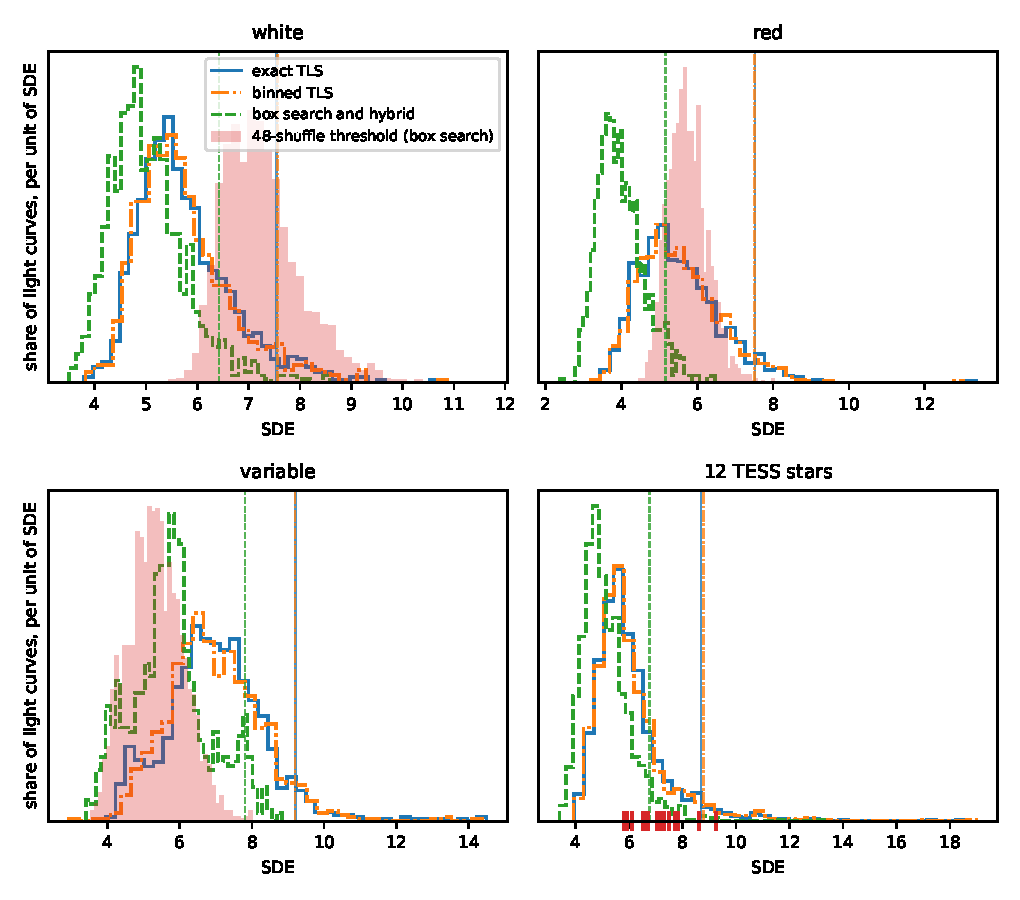
\includegraphics[width=0.8\textwidth]{null_sde.pdf}
\caption{The SDE of the noise-only light curves of the recovery test (Sect.~\ref{sec:recovery}) for exact mode, binned mode and the box search, in each noise class and on the 12 real TESS stars, with the threshold of each search at a false-alarm rate of 5\% as a vertical line of its colour; the hybrid has the SDE of the box search. The shaded distribution is the 48-shuffle threshold of the box search from the calibration light curves of Table~\ref{tab:null}, which are a different set from the same generator; on the real stars each mark is one star's threshold, the 12 stars of Sect.~\ref{sec:realstars} and the eight further stars of the exchangeability test.}\label{fig:nullsde}
\end{figure}

\begin{figure}[htbp]
\centering
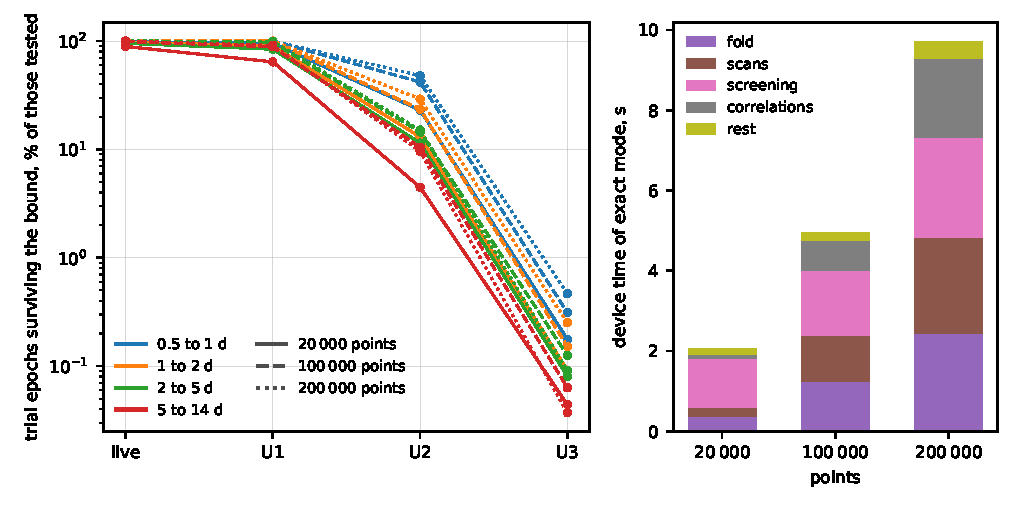
\includegraphics[width=\textwidth]{funnel.pdf}
\caption{Left: the share of the trial epochs that survive each bound of the screening cascade (live, $U_1$, $U_2$, $U_3$) in each period range at the three sizes of Table~\ref{tab:funnel}, summed over the template lengths. Right: the GPU time of exact mode over the period grid by stage, from the profiler, at the three sizes of Table~\ref{tab:split}.}\label{fig:funnel}
\end{figure}

\clearpage
\section{Reproducibility}\label{sec:repro}
Every number measured for this paper comes from a command of the repository, run from its root with the GPU group installed (\texttt{uv sync --group rocm}; the figure scripts also need the \texttt{examples} extra). The commands that run a search need the GPU; the scripts that write the tables, the macros and the PDF from the recorded files do not.
\begin{itemize}
\item Agreement with TLS on its 14 characterization cases, and Table~\ref{tab:validation}: \texttt{uv run pytest tests/test\_tls\_golden.py} and \texttt{uv run python paper/scripts/validation.py}.
\item The adversarial cases of Sect.~\ref{sec:adversarial}: \texttt{uv run pytest tests/test\_tls\_adversarial.py}, which runs TLS fused on the CPU as the reference, and \texttt{uv run python paper/scripts/adversarial.py}, which writes the largest differences measured to \texttt{paper/adversarial\_table.json}.
\item Table~\ref{tab:binned}: \texttt{uv run python paper/scripts/binned\_accuracy.py}.
\item Table~\ref{tab:funnel} and the share of trial epochs that reach the exact correlation: \texttt{taskset -c 0-15 uv run python paper/scripts/screening\_stats.py --json paper/scripts/screening\_stats.json}. Table~\ref{tab:split}: \texttt{taskset -c 0-15 uv run python paper/scripts/profile\_split.py --json paper/scripts/profile\_split.json}.
\item Table~\ref{tab:cpu}, the times of Sect.~\ref{sec:time} and the rows of Sect.~\ref{sec:gtlstime}: one session of \texttt{bash benchmarks/session.sh DIRECTORY}, which runs \texttt{benchmarks/bench.py} once for each part (the rows of the table, the set of 64 light curves, the shuffles, the light curves of the GTLS benchmark at both trial-epoch margins, the first call of a fresh process of Sect.~\ref{sec:time} and the profile of Table~\ref{tab:split}, by the same script as the item above), then \texttt{uv run python benchmarks/assemble.py DIRECTORY --out benchmarks/results.json}; the command, the rows and the number of calls of every part are recorded in that file, and the synthetic light curves are made by the script with the seed 20260101. Table~\ref{tab:split} itself: \texttt{uv run python paper/scripts/split\_table.py paper/scripts/profile\_split.json}.
\item Fig.~\ref{fig:completeness} and Table~\ref{tab:recovery}: \texttt{uv run python validation/run.py PART DIRECTORY} for each part (main-white, main-red and main-variable) and \texttt{uv run python validation/analyse.py DIRECTORY}; binned mode on the same light curves by \texttt{uv run python validation/rerun\_binned.py PART RERUN\_DIRECTORY} for each part and \texttt{uv run python validation/analyse\_binned.py RERUN\_DIRECTORY DIRECTORY}, put in place of the first binned rows by \texttt{uv run python paper/scripts/merge\_recovery.py DIRECTORY/results.json RERUN\_DIRECTORY/results-bands.json --out paper/recovery.json}; then the real part by \texttt{uv run python validation/run.py real DIRECTORY\_REAL} and \texttt{uv run python validation/analyse.py DIRECTORY\_REAL}, whose \texttt{results.json} is \texttt{paper/recovery\_real.json}; then \texttt{uv run python paper/scripts/completeness.py paper/recovery.json --real paper/recovery\_real.json}.
\item Tables~\ref{tab:null} and \ref{tab:injection}: \texttt{uv run python validation/threshold.py} for the rows (the modes null, inj and real; the red and variable classes are flattened first by its \texttt{prepare} mode into a directory given as \texttt{--cache}, and the real mode fetches the light curves of \texttt{validation/stars.json} through \texttt{validation/fetch.py}) and \texttt{uv run python validation/threshold\_analysis.py ROWS --json paper/threshold.json}; then \texttt{uv run python paper/scripts/threshold\_table.py paper/threshold.json} and \texttt{uv run python paper/scripts/fill\_numbers.py}.
\item Table~\ref{tab:period}: \texttt{uv run python paper/scripts/period\_table.py paper/recovery.json --real paper/recovery\_real.json} (no GPU).
\item Fig.~\ref{fig:roc}: \texttt{uv run python validation/roc.py DIRECTORY --bands RERUN\_DIRECTORY --real DIRECTORY\_REAL} on the directories of Fig.~\ref{fig:completeness}, which writes \texttt{paper/roc.json}, then \texttt{uv run python paper/scripts/roc.py} (no GPU).
\item Table~\ref{tab:bins}: \texttt{uv run python paper/scripts/bins\_share.py}.
\item The three box searches on the variable class (Sect.~\ref{sec:recovery}): \texttt{uv run python validation/box\_variable.py OUTPUT\_DIRECTORY DIRECTORY --out paper/box\_variable.json}, on the evaluation directory of Fig.~\ref{fig:completeness}.
\item The attained column of Table~\ref{tab:hardware}: \texttt{uv run python benchmarks/peak.py --spec-bandwidth 960 --json paper/peak.json}, with the device otherwise idle.
\item Fig.~\ref{fig:wasp18}: \texttt{uv run python examples/plot\_wasp18.py}, on \texttt{examples/data/wasp18\_s2.npz}.
\item The macros of the paper: \texttt{uv run python paper/scripts/fill\_numbers.py} writes \texttt{paper/numbers.tex} from \texttt{benchmarks/results.json}, \texttt{paper/split\_numbers.tex} from \texttt{paper/scripts/profile\_split.json}, \texttt{paper/recovery\_numbers.tex} from \texttt{paper/recovery.json} and \texttt{paper/threshold\_numbers.tex} from \texttt{paper/threshold.json} and \texttt{paper/peak\_numbers.tex} from \texttt{paper/peak.json}, and \texttt{uv run pytest tests/test\_paper\_numbers.py} checks that they agree with their sources (no GPU).
\item The PDF: \texttt{uv run python paper/build.py} (no GPU).
\end{itemize}
The software versions and the hardware are recorded in \texttt{results.json} and in Sect.~\ref{sec:hardware}.

\bibliographystyle{aasjournal}
\bibliography{refs}
\end{document}
